
%\pdfoutput=1 % only if pdf/png/jpg images are used
%\documentclass[a4paper,10pt]{article}
\documentclass[a4paper,10pt]{scrartcl}
%\documentclass[smallcondensed,referee]{svjour3}
\usepackage{geometry}
\geometry{a4paper,left=25mm,right=25mm, top=24mm, bottom=32mm}
%\geometry{a4paper}
\raggedbottom
\widowpenalty=10000
\clubpenalty=10000 
\usepackage{graphics}  
\usepackage{graphicx}
\usepackage{subfigure}
\usepackage{amsmath}
\usepackage{amssymb}
%\usepackage[amssymb]{SIunits}
\usepackage[load-configurations=abbreviations,tight-spacing=true,separate-uncertainty,bracket-numbers = false]{siunitx} % JINST cannnot handle siunitx !!
\usepackage{nicefrac}
\usepackage[english]{babel}
\usepackage{lineno}
%linenumbers
\setpagewiselinenumbers
\modulolinenumbers[5]
%\setlength\columnsep{25pt}
\usepackage{epstopdf}
\usepackage{stfloats}
%\usepackage{upgreek}
\usepackage{verbatim}
\usepackage{url}
\usepackage{xcolor}
%\usepackage{draftwatermark}
%\SetWatermarkScale{5}
\usepackage{setspace}
\usepackage{multicol,caption}
\usepackage{booktabs}
%\usepackage{ulem}

%charges
\newcommand{\q}{\ensuremath{\mathnormal{q}}}
\newcommand{\e}{\ensuremath{\mathnormal{e}}}
\newcommand{\h}{\ensuremath{\mathnormal{h}}}
\newcommand{\Qo}{Q_{\textrm{out}}}
\newcommand{\Qin}{Q_{\textrm{in}}}
\newcommand{\Qtot}{Q_{\textrm{tot}}}
\newcommand{\qo}{q_{\textrm{out}}}
\newcommand{\qin}{q_{\textrm{in}}}
\newcommand{\qtot}{q_{\textrm{tot}}}
\newcommand{\Vo}{V_{\textrm{out}}}
\newcommand{\Vin}{V_{\textrm{in}}}
\newcommand{\Vtot}{V_{\textrm{tot}}}

%TCT
\newcommand{\aITC}{\ensuremath{\alpha}\textrm{-TCT}}
\newcommand{\bITC}{\ensuremath{\beta}\textrm{-TCT}}
\newcommand{\mipITC}{\textrm{MIP-TCT}}
\newcommand{\drift}{{\textrm{drift}}}
\newcommand{\plasma}{{\textrm{plasma}}}
\newcommand{\p}{{\textrm{p}}}
\newcommand{\phonon}{{\textrm{phon}}}
\newcommand{\cph}{c_{\phonon}}

\newcommand{\dpen}{\delta_{\textrm{p}}}
\newcommand{\lir}{l_{\textrm{ir}}}

%times
\newcommand{\ttr}{\mathnormal{t'}}
\newcommand{\tdt}{\mathnormal{\tau}_{\textrm{dt}}}
\newcommand{\taup}{\mathnormal{\tau}_{\textrm{p}}}
\newcommand{\tp}{\mathnormal{t}_{\textrm{p}}}
\newcommand{\trap}{\textrm{trap}}
\newcommand{\tautr}{\mathnormal{\tau}_{\trap}}
\newcommand{\ttd}{\mathnormal{\tau}_{\trap}^{\drift}}
\newcommand{\tlife}{\tau_\textrm{life}}
\newcommand{\tfree}{\tau_\textrm{free}}
\newcommand{\tth}{\tau_\textrm{th}}
\newcommand{\trecgamma}{\tau_\textrm{rec}^{\gamma}}
\newcommand{\ttrans}{\tau_\textrm{trans}}
\newcommand{\trel}{\tau_\textrm{rel}}
\newcommand{\tR}{\tau_\textrm{R}}
\newcommand{\tRe}{\tau_{\textrm{R},\e}}
\newcommand{\tRh}{\tau_{\textrm{R},\h}}
\newcommand{\tcool}{\mathnormal{\tau}_{\textrm{cool}}}

\newcommand{\tauzero}{\tau_{0}}
\newcommand{\tauzeroprime}{\tau_{0}^{\prime}}
\newcommand{\tauoneprime}{\tau_{1}^{\prime}}
\newcommand{\tauone}{\tau_{1}}
\newcommand{\taub}{\tau_{\textrm{b}}}
\newcommand{\taudrift}{\tau_{\textrm{d}}}
\newcommand{\tauevap}{\tau_\textrm{e}}
\newcommand{\taurec}{\tau_\textrm{r}}
\newcommand{\taurelax}{\tau_\textrm{relax}}
\newcommand{\tauscat}{\tau_\textrm{scat}}

%velocities
\newcommand{\vth}{\mathnormal{v}_{\textrm{th}}}
\newcommand{\vsat}{v_{\textrm{sat}}}
\newcommand{\vsate}{v_{\textrm{sat}}^{\e}}
\newcommand{\vsath}{v_{\textrm{sat}}^{\h}}
\newcommand{\vdrift}{v_{\textrm{drift}}}
\newcommand{\vdrifte}{v_{\textrm{drift}}^{\e}}
\newcommand{\vdrifth}{v_{\textrm{drift}}^{\h}}
\newcommand{\vrel}{v_{\textrm{rel}}}

\newcommand{\vrelax}{v_\textrm{relax}}
\newcommand{\vt}{v_{\textrm{t}}}
\newcommand{\vl}{v_{\textrm{l}}}

%mobilities
\newcommand{\muaps}{\mu_{\textrm{APS}}}
\newcommand{\muiis}{\mu_{\textrm{IIS}}}
\newcommand{\munis}{\mu_{\textrm{NIS}}}

\DeclareMathOperator{\Erf}{{\textrm{Erf}}}
\DeclareMathOperator{\Erfc}{{\textrm{Erfc}}}

\newcommand{\kB}{k_{\textrm{B}}}

%energies
\newcommand{\Ex}{E_{\textrm{x}}}
\newcommand{\Exsi}{E_{\textrm{x}}^{\textrm{Si}}}
\newcommand{\Ec}{E_{\textrm{C}}}
\newcommand{\Ea}{E_{\textrm{a}}}
\newcommand{\EA}{E_{\textrm{A}}}
\newcommand{\ED}{E_{\textrm{D}}}
\newcommand{\Ei}{E_{\textrm{i}}}
\newcommand{\Ev}{E_{\textrm{V}}}
\newcommand{\Eg}{E_{\textrm{g}}}
\newcommand{\Etot}{E_{\textrm{tot}}}
\newcommand{\Uel}{U_{\textrm{el}}}
\newcommand{\Tnuc}{T_{\textrm{nuc}}}
\newcommand{\Eopt}{E_{\textrm{opt}}}
\newcommand{\EF}{E_{\textrm{F}}}
\newcommand{\EFe}{E_{\textrm{F}}^\e}
\newcommand{\EFh}{E_{\textrm{F}}^\h}
\newcommand{\Epair}{E_{\textrm{pair}}}
\newcommand{\Ephon}{E_{\textrm{ph}}}

%densities
\newcommand{\ndosv}{\mathnormal{n}_{\textrm{dos,v}}}
\newcommand{\ndosc}{\mathnormal{n}_{\textrm{dos,c}}}
\newcommand{\No}{N_{\textrm{out}}}
\newcommand{\Nin}{N_{\textrm{in}}}
\newcommand{\Ntot}{N_{\textrm{tot}}}
\newcommand{\no}{n_{\textrm{out}}}
\newcommand{\nexit}{n_{\textrm{exit}}}
\newcommand{\nin}{n_{\textrm{in}}}
\newcommand{\ntot}{n_{\textrm{tot}}}
\newcommand{\nee}{n_{\e}}
\newcommand{\nh}{n_{\h}}
\newcommand{\Nphon}{N_{\textrm{ph}}}

\newcommand{\ndrift}{n_{\drift}}
\newcommand{\nt}{n_{\textrm{t}}}
\newcommand{\nl}{n_{\textrm{l}}}

%boltzmans
\newcommand{\expmEx}{\exp{\left(-\Ex/\kB T \right)}}
\newcommand{\exppEx}{\exp{\left( \Ex/\kB T \right)}}
\newcommand{\expmEa}{\exp{\left(-\Ea/\kB T \right)}}
\newcommand{\exppEa}{\exp{\left( \Ea/\kB T \right)}}
\newcommand{\expm}{\exp{\left(-\Delta/\kB T \right)}}
\newcommand{\expp}{\exp{\left( \Delta/\kB T \right)}}

%misc
\newcommand{\dd}{\mathrm d}
\newcommand{\lD}{\lambda_{\textrm{Debye}}}
\newcommand{\bias}{\textrm{bias}}
\newcommand{\X}{\textrm{x}}
\newcommand{\rrec}{r_\textrm{rec}}
\newcommand{\nE}{E\!\!\!\!/}
\newcommand{\pro}{\mathnormal{p}}
\newcommand{\vect}[1]{\boldsymbol{#1}}
\newcommand{\vk}{\vect{k}}
\newcommand{\vr}{\vect{r}}
\newcommand{\vph}{v_{\textrm{ph}}}
\newcommand{\vpht}{v_{\textrm{ph,t}}}
\newcommand{\vphl}{v_{\textrm{ph,l}}}

%masses
\newcommand{\mstar}{m^{*}}
\newcommand{\mestar}{m^{*}_{\e}}
\newcommand{\mhstar}{m^{*}_{\h}}
\newcommand{\melstar}{m^{*}_{\e,\textrm{l}}}
\newcommand{\metstar}{m^{*}_{\e,\textrm{t}}}
\newcommand{\mhh}{m_{\h,\textrm{h}}}
\newcommand{\mhl}{m_{\h,\textrm{l}}}
\newcommand{\ml}{m_{\e,\textrm{l}}}
\newcommand{\mt}{m_{\e,\textrm{t}}}
\newcommand{\mdose}{m_{\textrm{dos},\e}}
\newcommand{\mdosh}{m_{\textrm{dos},\h}}

\newcommand{\Tiv}{T_{\textrm{iv}}}
\newcommand{\Tc}{T_{\textrm{c}}}

\newcommand{\mut}{\mu_{\textrm{t}}}
\newcommand{\mul}{\mu_{\textrm{l}}}

%conditional compilation
\newcommand*{\notFORPAPER}{}%

\DeclareSIUnit\e{\ensuremath{\mathnormal{e}}}
\DeclareSIUnit\ext{\ensuremath{\mathrm{ext}}}
\DeclareSIUnit\pro{\ensuremath{\mathnormal{p}}}
\DeclareSIUnit\c{\ensuremath{\mathnormal{c}}}
\DeclareSIUnit\sample{\ensuremath{\mathrm{S}}}
\DeclareSIUnit\bunch{\ensuremath{\mathrm{bunch}}}
\DeclareSIUnit\ppb{\ensuremath{\mathrm{ppb}}}
\DeclareSIUnit\eh{\ensuremath{\mathrm{eh}}}
\DeclareSIUnit\pair{\ensuremath{\mathrm{pair}}}
\DeclareSIUnit\pairs{\ensuremath{\mathrm{pairs}}}
\DeclareSIUnit\muon{\ensuremath{\mu}}
\DeclareSIUnit\ADC{\ensuremath{\mathrm{ADC}}}


\makeatletter
\renewcommand{\maketitle}{\bgroup\setlength{\parindent}{0pt}
\begin{center}
  \vspace*{10mm}
  {\textbf{\huge\sffamily\@title}\par}
  \vspace{5mm}
   
  \large \@author 
  \vspace{5mm}
  \@date
\end{center}\egroup
}
\def\@xfootnote[#1]{%
  \protected@xdef\@thefnmark{#1}%
  \@footnotemark\@footnotetext}
\makeatother


%%%%%%%%%%%%%%%%%%%%%%%%%%%%%%%%%%%%%%%%%%%%%%%%55
%begin document
\begin{document}


\title{Modelling transient current measurements in single-crystal chemical vapour deposition diamond {\color{red}(A1)}}
%\title{Modelling temperature- and electric field-dependent transient current measurements in single-crystal chemical-vapour-deposition diamond}
%\title{Modelling temperature- and electric field-dependent time-of-flight measurements of electrons and holes in single-crystal CVD diamond}
\author{
 R.~Sauer${}^{\textrm{a,}}$\footnote[*]{rolf.sauer@uni-ulm.de},
H.~Jansen${}^{\textrm{b,}}$\footnote[\dag]{hendrik.jansen@desy.de}\\
%FIXME Wermes, Pernegger
\vspace{5mm}
${}^{\textrm{a}}$ Institut f\"ur Quantenmaterie/Halbleiterphysik, Ulm, Germany\\
${}^{\textrm{b}}$ Deutsches Elektronen-Synchrotron, Hamburg, Germany\\
}
\date{\today}
\maketitle
\tableofcontents

%\newpage
\linenumbers
\begin{abstract}
\noindent

Temperature- and electric field-dependent transient current experiments were reported recently and were used to extract drift mobilities and drift velocities of electrons and holes in commercially
 available single-crystal CVD diamonds. 
These data, available from room temperature down to 2\,K, show characteristic temperature-dependent current profiles and
  hint to an intermediate charge carrier storage process that has yet not been explained in detail. 
Here we present largely enriched experimental data and explain all observed phenomena by a detailed physical model. 
It is based on coupled rate equations and demonstrates the storage process to consist in the formation of free excitons (FE) and electron-hole droplets (EHD)
 prior to thermal activation and dissociation at increasing temperatures yielding the measured currents. 
The model describes all experimental findings satisfactorily, some of them quantitatively including the activation energy of 130\,meV
 and the temperature dependence of the total charge reaching the electrodes after drifting across the crystal. 
Maxima in the electron transit time versus temperature observed to become successively more prominent at low electric fields are also well understood in the frame of the model. 
They are ascribed to a valley re-population effect due to impurity-assisted inter-valley scattering.


\end{abstract}

%\tableofcontents


\part{Experimental data}

%\begin{multicols}{2}
\section{Introduction}
\label{sec:intro}
\ifdefined\notFORPAPER

In high-energy physics, semiconductors are used as solid-state ionisation chambers for charged particle detection profiting from their versatility. 
Besides well-established silicon-based sensors, diamond detectors are an emergent technology due to their exceptional electrical properties~\cite{book:PhysApplCVD}. 
Diamond is a wide band gap semiconductor and in the field of high-energy physics its usage growths steadily due to its radiation hardness and usability in harsh environments. 
Remarkable properties as high breakdown fields and low leakage currents are a direct result from its wide band gap of ($\SI{5.47}{\eV}$)~\cite{1964} 
 rendering very precise signal current measurements possible. 

Excitonic properties in various semiconductors are usually studied using optical methods detecting the photon emitted during the exciton's radiative decay. 
Therefore, those excitons that thermally dissociate elude optical detection. 
In this work, the experimental set-up resembles a charged particle detection experiment. 
We therefore measure the current induced from drifting charge carriers in an externally applied electric field, i.e.\ the thermally dissociated excitons,
 which represent the complementary part to those radiatively recombined excitons. 
To this end, we apply the transient current technique (TCT), which has frequently been used for the determination of the charge carrier drift
 time in different materials \cite{TCT,Eremin1996388,pernegger:073704,PSSA:PSSA200561929,Fink2006227,PSSA:PSSA200561915}.

We discuss previously reported data \cite{jansen:173706} under new aspects including an excitonic model describing the temperature and electric field dependence of the measured transients. 
In order to explain the measurements in a wide range of electric field strengths and sample temperature our model includes the interplay of electron-hole-droplets (EHD), free excitons
 and free charge carriers, which are interconnected by various time constants. 
 
The paper is structured as follows:
We present the experimental technique in section~2 and the measured current profiles as a function of the temperature and the electric field strength in section~3. 
These current profiles are further analysed in terms of collected charge, shape and drift time. 
Section~4 discusses a physical model describing the data. 
\else

In high-energy physics, semiconductors are used as solid-state ionisation chambers for charged particle detection profiting from their versatility. 
Besides well-established silicon-based sensors, diamond detectors are an emergent technology due to their exceptional electrical properties~\cite{book:PhysApplCVD}. 
Diamond is a wide band gap semiconductor and in the field of high-energy physics its usage growths steadily due to its radiation hardness and usability in harsh environments. 
Remarkable properties as high breakdown fields and low leakage currents are a direct result from its wide band gap of ($\SI{5.47}{\eV}$)~\cite{1964} 
 rendering very precise signal current measurements possible. 

Excitonic properties in various semiconductors are usually studied using optical methods detecting the photon emitted during the exciton's radiative decay. 
Therefore, those excitons that thermally dissociate elude optical detection. 
In this work, the experimental set-up resembles a charged particle detection experiment. 
We therefore measure the current induced from drifting charge carriers in an externally applied electric field, i.e.\ the thermally dissociated excitons,
 which represent the complementary part to those radiatively recombined excitons. 
To this end, we apply the transient current technique (TCT), which has frequently been used for the determination of the charge carrier drift
 time in different materials \cite{TCT,Eremin1996388,pernegger:073704,PSSA:PSSA200561929,Fink2006227,PSSA:PSSA200561915}.

We discuss previously reported data \cite{jansen:173706} under new aspects including an excitonic model describing the temperature and electric field dependence of the measured transients. 
In order to explain the measurements in a wide range of electric field strengths and sample temperature our model includes the interplay of electron-hole-droplets (EHD), free excitons
 and free charge carriers, which are interconnected by various time constants. 
 
The paper is structured as follows:
We present the experimental technique in section~2 and the measured current profiles as a function of the temperature and the electric field strength in section~3. 
These current profiles are further analysed in terms of collected charge, shape and drift time. 
Section~4 discusses a physical model describing the data. 
\fi 

\section{Experimental technique}
\label{sec:ET}
\ifdefined\notFORPAPER

\subsection{The transient current technique}

In transient current experiments, also referred to as time-of-flight experiments,
 time-resolved currents are recorded that are induced on a read-out electrode by the drift of free charge carriers in an externally applied electric field. 
The sensor current induced by moving charges is elegantly formulated by the Shockley-Ramo theorem\,\cite{1686997}.
It makes use of a \textit{weighting potential} $\Phi_{\textrm{w}}$ which describes the coupling of a charge to an electrode.
The weighting potential therefore depends on the electrode configuration. 
Note that the weighting field $E_\textrm{w}$ is not to be confused with the electric field $E$: $\vect{\nabla}\Phi_{\textrm{w}} = - \vect{E}_{\textrm{w}} \neq - \vect{E}$.
With the number of drifting charges $Q$ and their trajectory $\vect{r}(t)$, the induced current reads

\begin{equation}
 i(t) = Q(t) \vect{\nabla}\Phi_{\textrm{w}} \frac{\dd}{\dd t}\vect{r}(t) = - Q(t) \vect{E_{\textrm{w}}} \vect{v}. 
\end{equation}

\noindent
In a parallel plate configuration the weighting field reduces to be $\vect{E_{\textrm{w}}} =  -\frac{\dd \Phi_{\textrm{w}}}{\dd x}= -1/d$ with the plate distance $d$. 
For a one-dimensional charge drift in an electric field of constant strength and with $Q(t) = \e \cdot N(t)$, the current density reads

\begin{equation}
  i(t) = \e \cdot N(t) \cdot \vdrift / d.
 \label{eq:ramo}
\end{equation}

The TCT provides direct way to derive the transit time of a localised charge cloud, i.e.~the time a charge cloud requires to drift through a crystal,
 from the time difference between the rising and the falling edge. 
This technique is usually, and also in this work, performed in a electrode-semiconductor-electrode structure.
Localised creation of free charges close to the electrode surface is realised by using highly ionising $\alpha$-particles with short penetration depth
 from an ${}^{241}\textrm{Am}$ source. 
Bragg-simulations based on NIST data \cite{NIST} show a penetration depth of approximately $\SI{10}{\micro\meter}$ for an $\alpha$-particle energy of $\SI{4.7}{\MeV}$,
 which is small compared to the sample thicknesses of about $\SI{500}{\micro\meter}$ used in this work. 
Transit times are of the order of few nanoseconds for such crystal sizes.
The drift of free charge carriers depends on the material's crystal properties and on the release mechanism from the initial charge cloud. 
Therefore, if the current is read with wide bandwidth, charge carrier properties and details about the release mechanism are accessible from the current pulse characteristics. 


\subsection{The measurement set-up}
The samples under test (SUT), which are referred to as \textit{S52}, \textit{S57}, and \textit{S79} for later reference, have been produced by chemical vapour deposition process
 by Element Six Ltd (E6) \cite{E6}.
The scCVD diamond samples have an area of $4.7 \times \SI{4.7}{\milli\meter^2}$
 and thicknesses of $d_{\textrm{S52}} = \SI{515}{\micro\meter}$, $d_{\textrm{S57}} = \SI{530}{\micro\meter}$, and $d_{\textrm{S79}} = \SI{529}{\micro\meter}$.
The dislocation and impurity densities are of the order of $\le \SI{2e14}{\centi\meter^{-3}}$. 
DDL quotes a nitrogen incorporation of $<\SI{1}{\ppb}$.
The leakage current is less than $\SI{7}{\pico\ampere}$ for $E = \pm \SI{1.1}{\volt/\micro\meter}$. 
In present scCVD diamond specimen, trapping times larger than $\SI{30}{\nano\second}$ have been realised \cite{pernegger:073704}. 

\begin{figure}[tb]
  \centering
  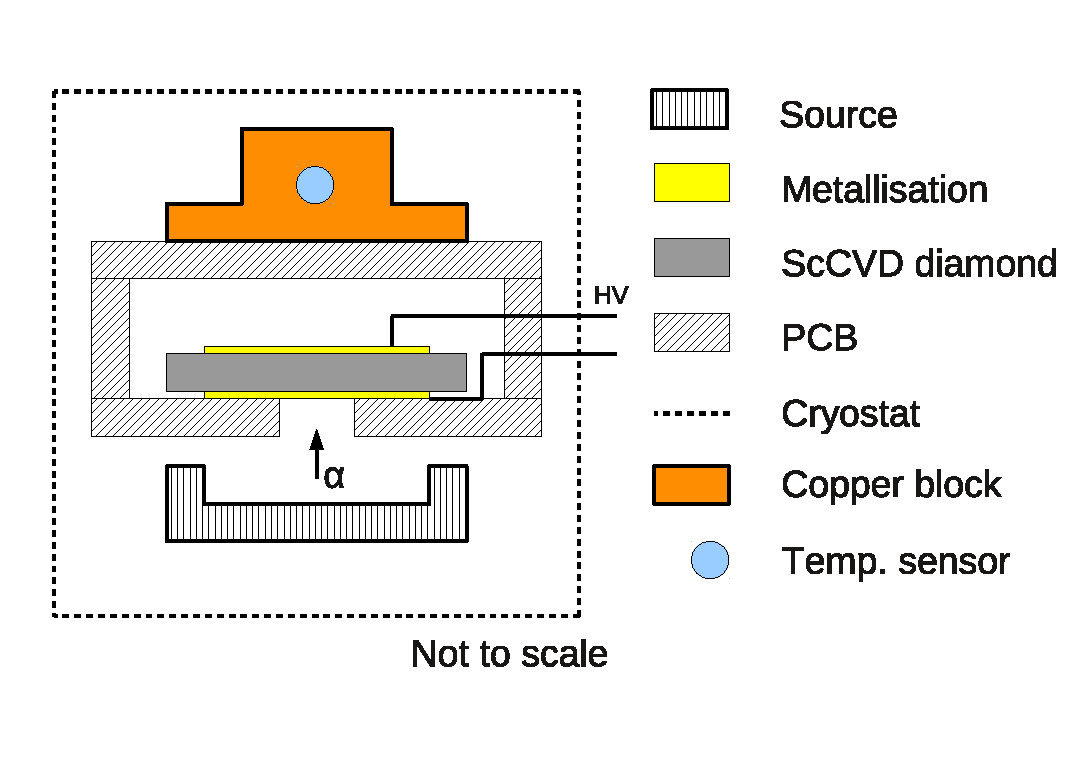
\includegraphics[trim=0cm 1.5cm 0cm 0.5cm, clip=true,width=0.45\textwidth]{./figures/diamond_collimator4.eps}

  \caption{The measuring unit is detailed. The thermal heater is omitted and is located behind the copper block.}
  \label{fig:SETUPtct}
\end{figure} %FIXME cryostat should read innver vacuum chamber in the plot

The set-up used for the presented measurements consists of a measuring unit, a digital oscilloscope, a thermal heater, and a liquid helium cryostat comprising an inner vacuum chamber (IVC). 
The measuring unit consists of a PCB sensor holder providing a backside contact to ground and a $\SI{50}{\ohm}$ read-out line, which also serves as high-voltage contact. 
The cryostat holds the liquid helium, the measuring unit is situated in the IVC,
 which has been evacuated prior to the measurements and then filled with helium gas to a pressure of $\sim\SI{5e-2}{\milli\bar}$.
This provides an excellent thermal contact whilst keeping the breakdown voltage high enough. 
Furthermore, a calibrated CERNOX temperature sensor at close vicinity to the SUT is thermally coupled to the PCB via a copper block. 
The sensor holder has a hole of $\textrm{\O} = \SI{1}{\milli\meter}$ at the bottom, collimating the $\alpha$-particles from the ${}^{241}\textrm{Am}$ source
 and ensuring that they impinge the sensor only within the metallised area.
A sketch of the cross section of the measuring unit is shown in Fig.~\ref{fig:SETUPtct}. %1 in reference \cite{ jansen:173706}.
The $\alpha$-particles emitted from the ${}^{241}\textrm{Am}$ %source have an energy of $\SI{5.48}{\MeV}$. 
reach the bulk with $\sim \SI{4.7}{\MeV}$,
 corresponding to $\num{3.5e5}$ created electron-hole (e-h) pairs in the diamond sample under the assumption of an average e-h pair creation energy of $\SI{13.25}{\eV}$\cite{4329650}. 
At the lowest absolute applied bias voltage ($\SI{30}{\volt}$), the sensor capacity is charged with $\SI{6e-11}{\coulomb}$ on the electrodes,
 or $\SI{3.7e8}{\e}$, which is much larger than the number of induced e-h pairs per $\alpha$-particle. 
Hence, the produced free charge carriers do not change significantly the electric field in the bulk region. 

Figure~\ref{fig:SETUPtct2} shows the electrical schematics of the set-up. 
The high voltage is applied to the top contact and is AC-coupled to the amplifier via a $\SI{1}{\nano\farad}$ capacitor. 
The electrical connection to the amplifier, which is located outside of the cryostat, is realised via a vacuum-tight feedthrough. 
As electron-hole (e-h) pairs are created close to the bottom contact,
 one charge carrier type is collected there almost instantly,
 whilst the other drifts through the entire bulk to reach the top contact. 
Hole (electron) induced currents are read if a negative (positive) bias voltage is applied to the top contact.

\begin{figure}[t]
  %\centering
  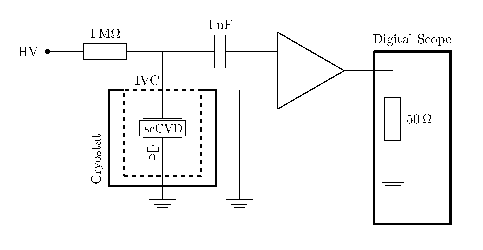
\includegraphics[width=0.45\linewidth]{./figures/circuit2}

   \caption{The electrical schematics of the TCT set-up are shown. 
   The diamond sample is situated in a vacuum chamber with electrical connections to the outside. 
   The vacuum chamber resides within the liquid helium cooled  cryostat.}
   \label{fig:SETUPtct2}
\end{figure}

A $\SI{2}{\giga\hertz}$ bandwidth, two-staged, bipolar transistor amplifier %with an amplification factor of $A_{\textrm{amp}} = (138\pm 7) $ at $\SI{3.3}{\pico\farad}$ input capacitance,
 is used to amplify the signal before it is read via an oscilloscope. 
The minimum resolvable rise time with a $\SI{2}{\giga\hertz}$ amplifier is $\SI{180}{\pico\second}$. 
The cut-off frequency at $\SI{-3}{\decibel}$ within a RC-circuit is $f_{\textrm{cut}} = 1/(2\pi R_{\textrm{in}} \left( C_{\textrm{d}}+C_{\textrm{stray}}\right))$. 
Including stray capacitances $f_{\textrm{cut}}\approx \SI{1}{\giga\hertz}$ is estimated. 
The signal from the read-out electrode is read via a $\SI{1.6}{\meter}$ long UT-85 cable to bring the signal out of the cryostat and via a 3.15\,m high quality coax-cable outside of the cryostat
 towards the oscilloscope.
The digitalisation is realised via a LeCroy\,WavePro\,7300A with $\SI{3}{\giga\hertz}$ analogue bandwidth at a sampling rate of $\SI{10}{\giga\sample/\second}$. 
Note that neither a bandwidth limitation nor filtering has been used. 
Only at small signal-to-noise ratios ($\textrm{SNR}<9$), i.e.~at low bias voltages where the rise times are $> \SI{2}{\nano\second}$, the bandwidth was limited to $\SI{200}{\mega\hertz}$,
 affecting the length of the current pulse by less than 1\,\%. 
In summary, the read-out system provides a sufficiently wide analogue bandwidth in order to resolve features in the current pulse of down to 360\,ps. 






\subsection{Data acquisition}

The oscilloscope's trigger settings were chosen such that individual pulses are recorded, when the pulse amplitude exceeds a certain threshold of few millivolt in coincidence with a
 signal width $> \nicefrac{2}{3}$ of the actual width.
The combination of the two conditions reduced the trigger rate of shot noise induced triggers to effectively zero without cutting any signal
 whilst maintaining a short measurement duration of a few minutes per voltage-temperature pair. 

For every given pair of temperature and bias voltage setting, 300 pulses were recorded within a time window of $\SI{200}{\nano\second}$ . 
In the offline analysis the individual signals are corrected for trigger jitter and combined to form an average pulse. 
Only signals with an $\textrm{SNR}> 3$ are considered in order to
 reject pick-up triggers induced e.g.~by other equipment in the laboratory. 


\else

\subsection{The transient current technique}

In transient current experiments, also referred to as time-of-flight experiments,
 time-resolved currents are recorded that are induced on a read-out electrode by the drift of free charge carriers in an externally applied electric field. 
The sensor current induced by moving charges is elegantly formulated by the Shockley-Ramo theorem\,\cite{1686997}.
It makes use of a \textit{weighting potential} $\Phi_{\textrm{w}}$ which describes the coupling of a charge to an electrode.
The weighting potential therefore depends on the electrode configuration. 
Note that the weighting field $E_\textrm{w}$ is not to be confused with the electric field $E$: $\vect{\nabla}\Phi_{\textrm{w}} = - \vect{E}_{\textrm{w}} \neq - \vect{E}$.
With the number of drifting charges $Q$ and their trajectory $\vect{r}(t)$, the induced current reads

\begin{equation}
 i(t) = Q(t) \vect{\nabla}\Phi_{\textrm{w}} \frac{\dd}{\dd t}\vect{r}(t) = - Q(t) \vect{E_{\textrm{w}}} \vect{v}. 
\end{equation}

\noindent
In a parallel plate configuration the weighting field reduces to be $\vect{E_{\textrm{w}}} =  -\frac{\dd \Phi_{\textrm{w}}}{\dd x}= -1/d$ with the plate distance $d$. 
For a one-dimensional charge drift in an electric field of constant strength and with $Q(t) = \e \cdot N(t)$, the current density reads

\begin{equation}
  i(t) = \e \cdot N(t) \cdot \vdrift / d.
 \label{eq:ramo}
\end{equation}

The TCT provides direct way to derive the transit time of a localised charge cloud, i.e.~the time a charge cloud requires to drift through a crystal,
 from the time difference between the rising and the falling edge. 
This technique is usually, and also in this work, performed in a electrode-semiconductor-electrode structure.
Localised creation of free charges close to the electrode surface is realised by using highly ionising $\alpha$-particles with short penetration depth
 from an ${}^{241}\textrm{Am}$ source. 
Bragg-simulations based on NIST data \cite{NIST} show a penetration depth of approximately $\SI{10}{\micro\meter}$ for an $\alpha$-particle energy of $\SI{4.7}{\MeV}$,
 which is small compared to the sample thicknesses of about $\SI{500}{\micro\meter}$ used in this work. 
Transit times are of the order of few nanoseconds for such crystal sizes.
The drift of free charge carriers depends on the material's crystal properties and on the release mechanism from the initial charge cloud. 
Therefore, if the current is read with wide bandwidth, charge carrier properties and details about the release mechanism are accessible from the current pulse characteristics. 


\subsection{The measurement set-up}
The samples under test (SUT), which are referred to as \textit{S52}, \textit{S57}, and \textit{S79} for later reference, have been produced by chemical vapour deposition process
 by Element Six Ltd (E6) \cite{E6}.
The scCVD diamond samples have an area of $4.7 \times \SI{4.7}{\milli\meter^2}$
 and thicknesses of $d_{\textrm{S52}} = \SI{515}{\micro\meter}$, $d_{\textrm{S57}} = \SI{530}{\micro\meter}$, and $d_{\textrm{S79}} = \SI{529}{\micro\meter}$.
The dislocation and impurity densities are of the order of $\le \SI{2e14}{\centi\meter^{-3}}$. 
DDL quotes a nitrogen incorporation of $<\SI{1}{\ppb}$.
The leakage current is less than $\SI{7}{\pico\ampere}$ for $E = \pm \SI{1.1}{\volt/\micro\meter}$. 
In present scCVD diamond specimen, trapping times larger than $\SI{30}{\nano\second}$ have been realised \cite{pernegger:073704}. 

\begin{figure}[tb]
  \centering
  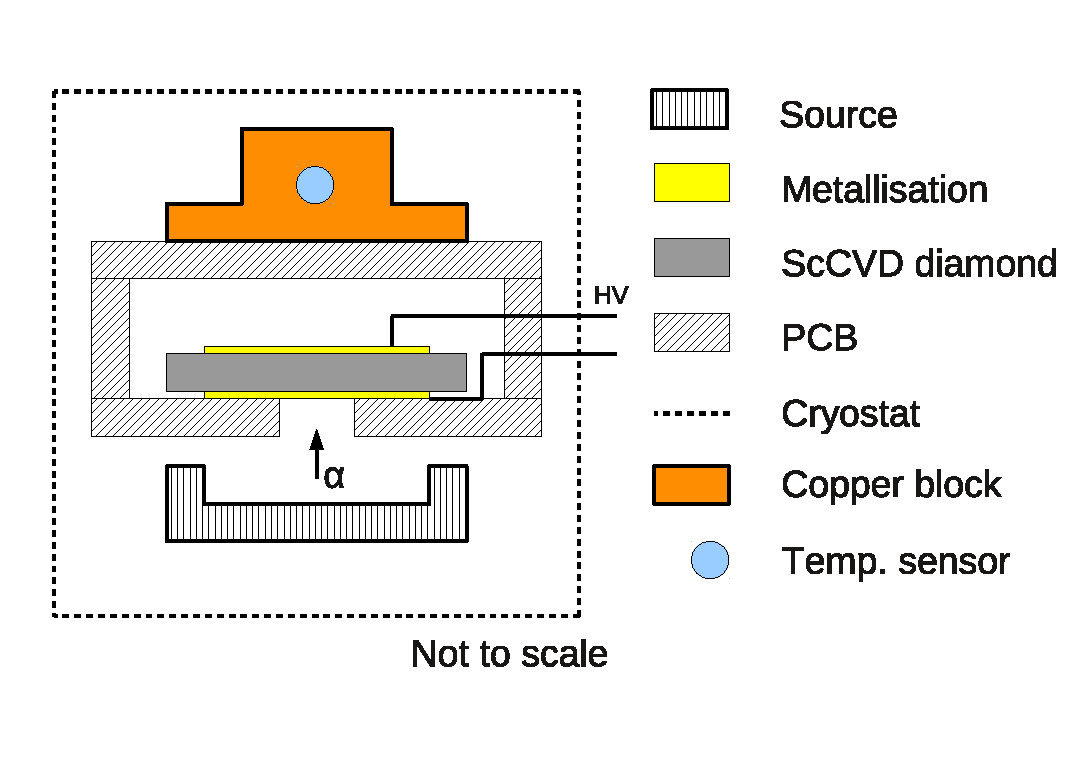
\includegraphics[trim=0cm 1.5cm 0cm 0.5cm, clip=true,width=0.45\textwidth]{./figures/diamond_collimator4.eps}

  \caption{The measuring unit is detailed. The thermal heater is omitted and is located behind the copper block.}
  \label{fig:SETUPtct}
\end{figure} %FIXME cryostat should read innver vacuum chamber in the plot

The set-up used for the presented measurements consists of a measuring unit, a digital oscilloscope, a thermal heater, and a liquid helium cryostat comprising an inner vacuum chamber (IVC). 
The measuring unit consists of a PCB sensor holder providing a backside contact to ground and a $\SI{50}{\ohm}$ read-out line, which also serves as high-voltage contact. 
The cryostat holds the liquid helium, the measuring unit is situated in the IVC,
 which has been evacuated prior to the measurements and then filled with helium gas to a pressure of $\sim\SI{5e-2}{\milli\bar}$.
This provides an excellent thermal contact whilst keeping the breakdown voltage high enough. 
Furthermore, a calibrated CERNOX temperature sensor at close vicinity to the SUT is thermally coupled to the PCB via a copper block. 
The sensor holder has a hole of $\textrm{\O} = \SI{1}{\milli\meter}$ at the bottom, collimating the $\alpha$-particles from the ${}^{241}\textrm{Am}$ source
 and ensuring that they impinge the sensor only within the metallised area.
A sketch of the cross section of the measuring unit is shown in Fig.~\ref{fig:SETUPtct}. %1 in reference \cite{ jansen:173706}.
The $\alpha$-particles emitted from the ${}^{241}\textrm{Am}$ %source have an energy of $\SI{5.48}{\MeV}$. 
reach the bulk with $\sim \SI{4.7}{\MeV}$,
 corresponding to $\num{3.5e5}$ created electron-hole (e-h) pairs in the diamond sample under the assumption of an average e-h pair creation energy of $\SI{13.25}{\eV}$\cite{4329650}. 
At the lowest absolute applied bias voltage ($\SI{30}{\volt}$), the sensor capacity is charged with $\SI{6e-11}{\coulomb}$ on the electrodes,
 or $\SI{3.7e8}{\e}$, which is much larger than the number of induced e-h pairs per $\alpha$-particle. 
Hence, the produced free charge carriers do not change significantly the electric field in the bulk region. 

Figure~\ref{fig:SETUPtct2} shows the electrical schematics of the set-up. 
The high voltage is applied to the top contact and is AC-coupled to the amplifier via a $\SI{1}{\nano\farad}$ capacitor. 
The electrical connection to the amplifier, which is located outside of the cryostat, is realised via a vacuum-tight feedthrough. 
As electron-hole (e-h) pairs are created close to the bottom contact,
 one charge carrier type is collected there almost instantly,
 whilst the other drifts through the entire bulk to reach the top contact. 
Hole (electron) induced currents are read if a negative (positive) bias voltage is applied to the top contact.

\begin{figure}[t]
  %\centering
  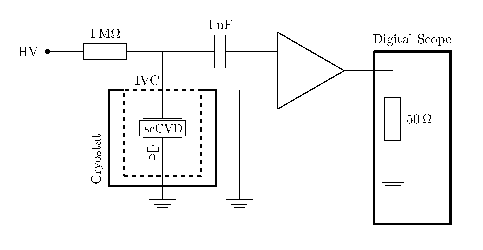
\includegraphics[width=0.45\linewidth]{./figures/circuit2}

   \caption{The electrical schematics of the TCT set-up are shown. 
   The diamond sample is situated in a vacuum chamber with electrical connections to the outside. 
   The vacuum chamber resides within the liquid helium cooled  cryostat.}
   \label{fig:SETUPtct2}
\end{figure}

A $\SI{2}{\giga\hertz}$ bandwidth, two-staged, bipolar transistor amplifier %with an amplification factor of $A_{\textrm{amp}} = (138\pm 7) $ at $\SI{3.3}{\pico\farad}$ input capacitance,
 is used to amplify the signal before it is read via an oscilloscope. 
The minimum resolvable rise time with a $\SI{2}{\giga\hertz}$ amplifier is $\SI{180}{\pico\second}$. 
The cut-off frequency at $\SI{-3}{\decibel}$ within a RC-circuit is $f_{\textrm{cut}} = 1/(2\pi R_{\textrm{in}} \left( C_{\textrm{d}}+C_{\textrm{stray}}\right))$. 
Including stray capacitances $f_{\textrm{cut}}\approx \SI{1}{\giga\hertz}$ is estimated. 
The signal from the read-out electrode is read via a $\SI{1.6}{\meter}$ long UT-85 cable to bring the signal out of the cryostat and via a 3.15\,m high quality coax-cable outside of the cryostat
 towards the oscilloscope.
The digitalisation is realised via a LeCroy\,WavePro\,7300A with $\SI{3}{\giga\hertz}$ analogue bandwidth at a sampling rate of $\SI{10}{\giga\sample/\second}$. 
Note that neither a bandwidth limitation nor filtering has been used. 
Only at small signal-to-noise ratios ($\textrm{SNR}<9$), i.e.~at low bias voltages where the rise times are $> \SI{2}{\nano\second}$, the bandwidth was limited to $\SI{200}{\mega\hertz}$,
 affecting the length of the current pulse by less than 1\,\%. 
In summary, the read-out system provides a sufficiently wide analogue bandwidth in order to resolve features in the current pulse of down to 360\,ps. 






\subsection{Data acquisition}

The oscilloscope's trigger settings were chosen such that individual pulses are recorded, when the pulse amplitude exceeds a certain threshold of few millivolt in coincidence with a
 signal width $> \nicefrac{2}{3}$ of the actual width.
The combination of the two conditions reduced the trigger rate of shot noise induced triggers to effectively zero without cutting any signal
 whilst maintaining a short measurement duration of a few minutes per voltage-temperature pair. 

For every given pair of temperature and bias voltage setting, 300 pulses were recorded within a time window of $\SI{200}{\nano\second}$ . 
In the offline analysis the individual signals are corrected for trigger jitter and combined to form an average pulse. 
Only signals with an $\textrm{SNR}> 3$ are considered in order to
 reject pick-up triggers induced e.g.~by other equipment in the laboratory. 


\fi



\section{Results}
\label{sec:InducedPulses}
\ifdefined\notFORPAPER

\subsection{Initial density estimation}

The impinging $\alpha$-particles create free charge carriers within a small volume of the diamond bulk. 
The ionisation volume is described by the penetration depth of the $\alpha$-particle and its radial size. 
An average penetration depth of $\dpen \approx \SI{10}{\micro\meter}$ is calculated making use of NIST data
 and the radial $1/e$ size is estimated to be $r_0 \approx \SI{2}{\nm}$. 
The short $r_0$ is a result of the amount of energy transferred from the primary $\alpha$-particle to the electrons, 
 which is of the order of 60\,eV, cf.\ \cite{JansenThesis}, section 3.1.1. 
The aspect ratio of the ionisation volume is roughly $\num{10000}/\num{2} = \num{5000}$. 
As is shown later, the amount of charge produced at room temperature is about $Q = \SI{52}{\femto\coulomb}$,
 matching an estimate of an $\alpha$-particle with $\SI{4.3}{\mega\eV}$ at an electron-hole-pair creation energy of $\SI{13.25}{\eV}$. 
The average charge density in the first radial $1/e$ length of the charge cloud in the instant of the impingement is hence estimated as 

\begin{equation}
 n = \frac{0.68\cdot\SI{52}{\femto\coulomb}}{r_0^2\pi \dpen} \approx \SI{5e21}{\pairs/\cm^{3}}.
\end{equation}

\subsection{Induced current pulses from carrier drift}
\begin{figure}[tb]
 \centering
 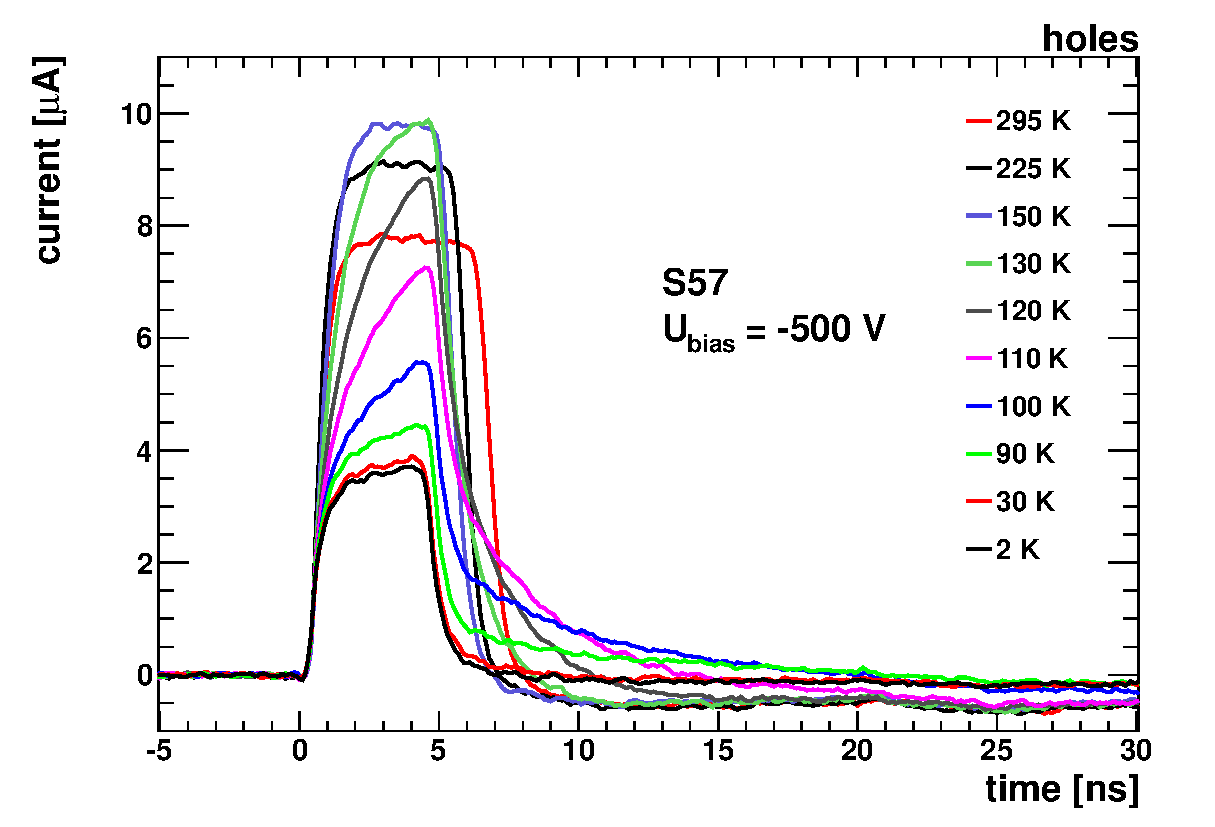
\includegraphics[width=0.49\textwidth]{figures/TCTholes500_exS57.eps}
 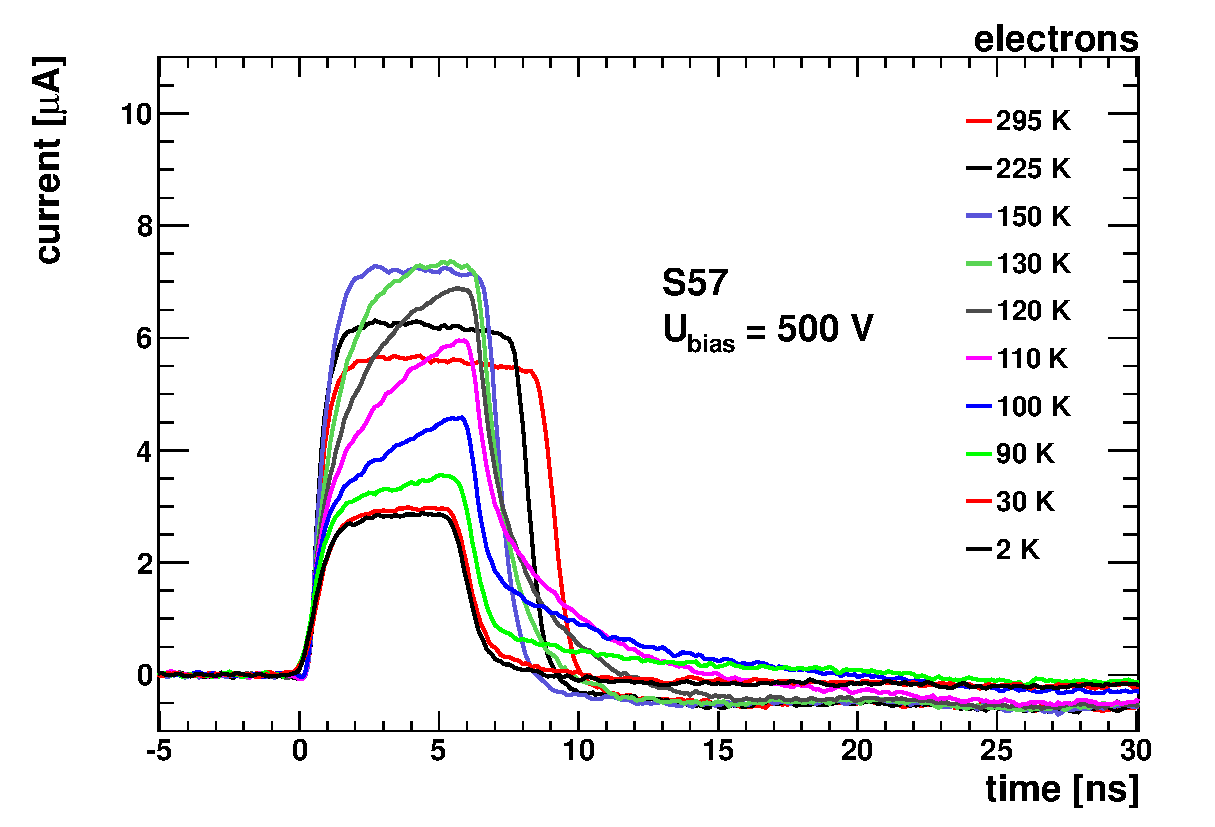
\includegraphics[width=0.49\textwidth]{figures/TCTelecs500_exS57.eps}
 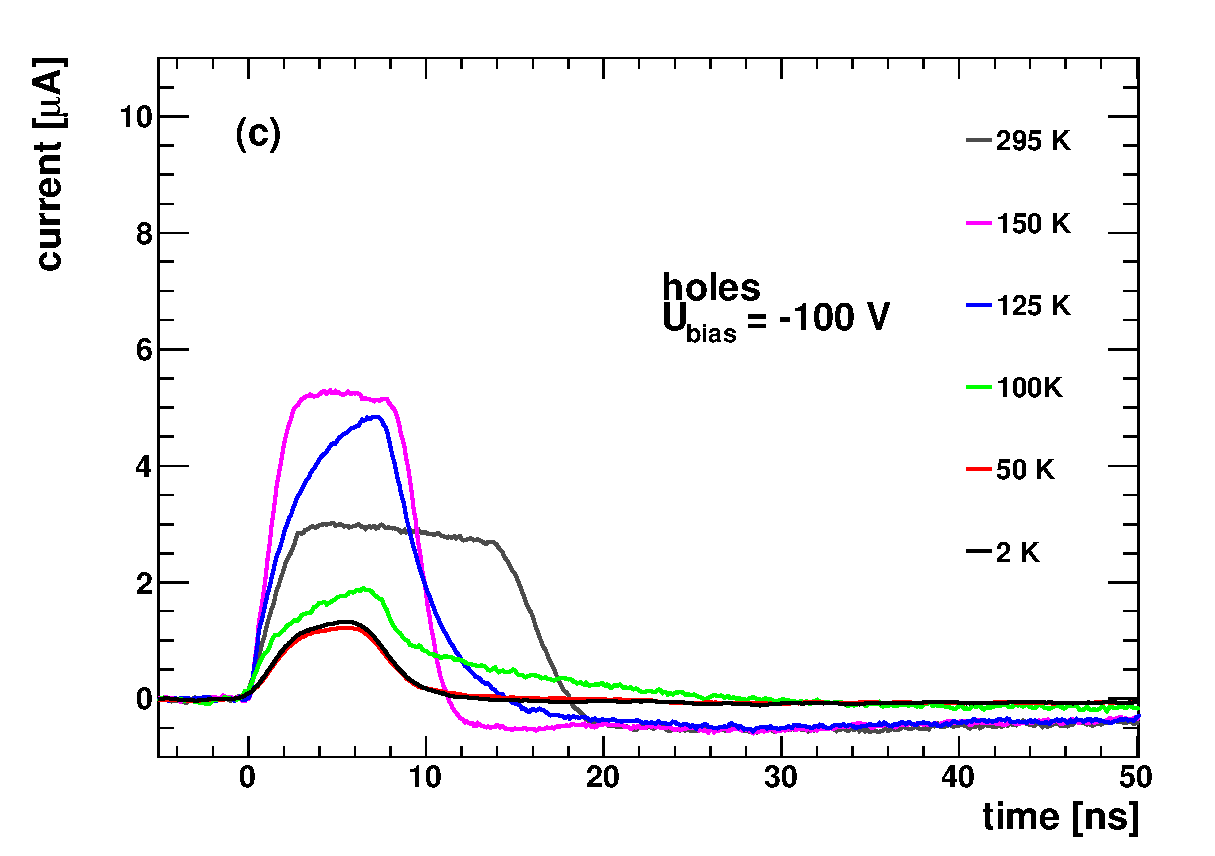
\includegraphics[width=0.49\textwidth]{figures/TCTholes100.eps}
 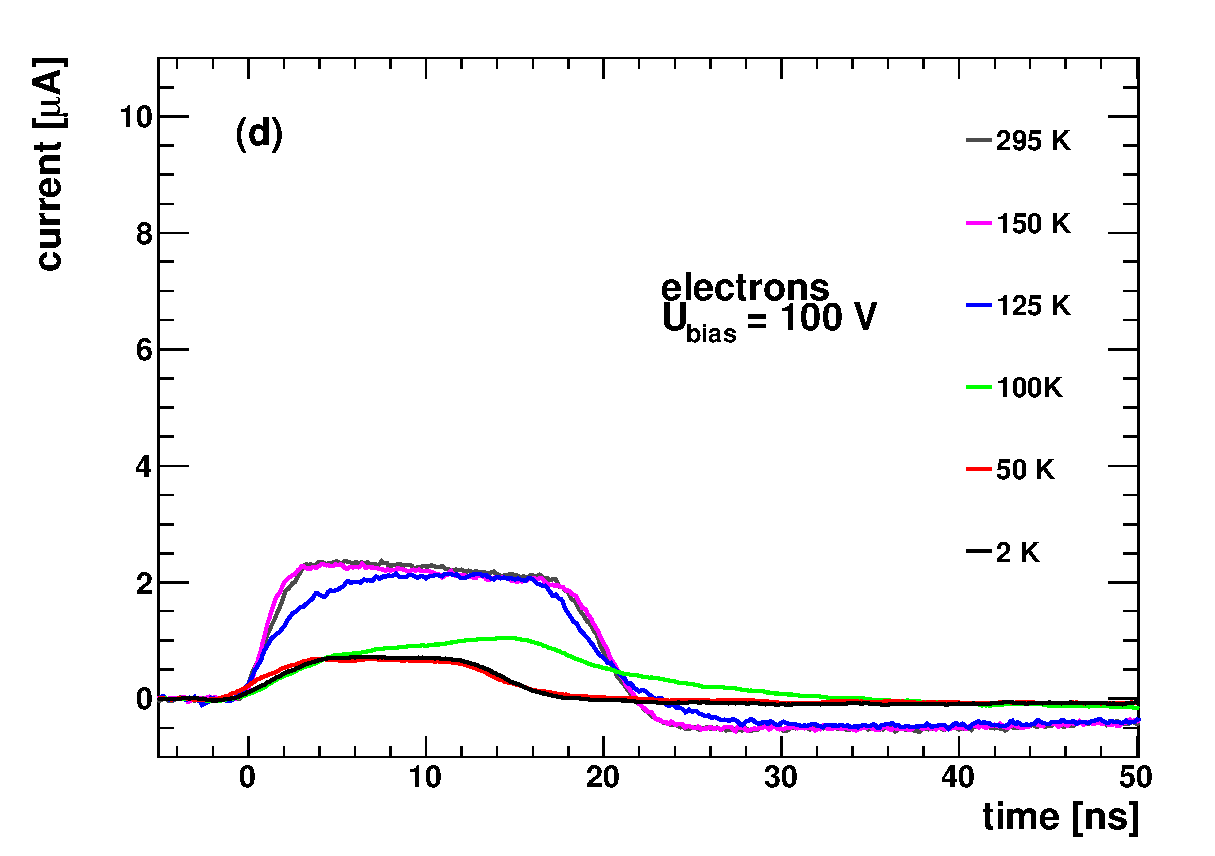
\includegraphics[width=0.49\textwidth]{figures/TCTelecs100.eps}

 \caption{Averaged current pulses for holes \textbf{(left column)} and electrons \textbf{(right column)} at various temperatures for
 $U_{\textrm{bias}} = \pm\SI{500}{\volt}$ \textbf{(top row)} and $U_{\textrm{bias}} = \pm\SI{100}{\volt}$ \textbf{(bottom row)} are shown for \textit{S57}.
 Note the similarity of electron pulses at $\SI{150}{\kelvin}$ and $\SI{295}{\kelvin}$. 
 Pulses from \textit{S52} and \textit{S79} are very similar and hence omitted.}
 \label{fig:currentprofiles}
\end{figure}

Hole and electron induced currents were recorded for temperatures between $T$ = 295\,K and  $\SI{2}{\kelvin}$. 
The set bias voltages covered a range from $ \SI{30}{\volt} \leq |V_{\textrm{bias}}| \leq \SI{900}{\volt}$ corresponding to electric field strengths from $\SI{0.06}{\volt/\um}$ to $\SI{1.8}{\volt/\um}$. 
Figure~\ref{fig:currentprofiles} shows a selection of the recorded and averaged pulses for SUT \textit{S57} at $\SI{\pm 500}{\volt}$ (top row) and $\SI{\pm 100}{\volt}$ (bottom row) for holes (left column)
 and electrons (right column). 
The electrons pulses are shown with an inverted current sign. 
Additional current pulses for samples \textit{S52} and \textit{S79} are published in \cite{JansenThesis}. 
At $\SI{\pm 500}{\volt}$, fast rise-times ($t_{\textrm{rise}} < \SI{1}{\nano\second}$) to about $\SI{2}{\micro\ampere}$  are observed for both hole and electron pulses for all temperatures. 
The time resolution for a single pulse (not averaged) at RT and $E = \SI{0.94}{\volt/\micro\meter}$ is $\sigma_{\textrm{t}} = \frac{\sigma_{\textrm{noise}}}{\textrm{slope}}
\leq \frac{\SI{0.4}{\micro\ampere}}{\nicefrac{\SI{7.2}{\micro\ampere}}{\SI{1}{\nano\second}}} = \SI{56}{\pico\second}$. 
At lower fields both the rise-time and the fall-time increase.

The rising edge of the signal marks the start of the charge drift. 
The falling edge marks the collection of charges at the opposite electrode. 
At RT the signal has an almost flat top during the drift as a consequence of the field being constant across our diamond samples. 
A net space-charge of the order of $\sim \SI{e11}{\e/\centi\meter^3}$ already leads to a significant change in pulse shape,
 i.e.~an exponential current behaviour~\cite{pernegger:073704}. 
Such intrinsic net space-charge seems to be absent in all three samples. 
For $\SI{\pm500}{\volt}$ ($E = \SI{0.94}{\volt/\micro\meter}$) the pulses become shorter with decreasing temperature
 due to higher carrier mobility as acoustic phonon scattering decreases with decreasing temperature.

The observed pulse shape depends strongly on the temperature between $\SI{75}{\kelvin}$ and $\SI{150}{\kelvin}$. 
The rising edge develops an $1-\exp \left(-t/\tau(T)\right)$ behaviour while the falling edge develops an equivalently long exponentially falling tail. 
Note that neither polarisation nor a non-zero net-effective space charge can explain the apparent temperature dependence of the shapes. 
The same effect on the pulse shape has been verified in all three SUTs.
A theoretical model explaining the temperature and electric field dependence of the pulse shape is laid down in the discussion section.
Here, we note that the signal can be decomposed into two parts: an almost rectangular one and a second comprising exponentially rising and falling flanks. 
The exponentially falling flank is a direct consequence of the exponentially rising flank. 

The drifting charges are collected at the opposing electrode after an average transit time $\ttr= \nicefrac{d}{\vdrift}$. 
This `release-drift-collect' scheme is depicted in Fig.~\ref{fig:collection} for two different start time distributions assuming a local charge deposition close to the incident electrode. 
If a function $\dot{N}_{\textrm{start}}(t)$ represents the distribution of the start time of the drift,
 the total number of charges that started to drift is $N_{\textrm{start}}(t) = \int_0^t \dot{N}_{\textrm{start}}(t)\,\dd t$. 
With the average transit time $\ttr = t_{\textrm{end}} - t_{\textrm{start}}$
 the distribution of the collection time of charges is $\dot{N}_{\textrm{end}}(t) = \dot{N}_{\textrm{start}}(t-\ttr)$, 
 and the total number of collected charges is $N_{\textrm{end}}(t) = \int_0^t \dot{N}_{\textrm{start}}(t-\ttr)\,\dd t$. 
The number of drifting charges is hence simply

\begin{equation}
 N_{\textrm{\drift}}(t) = N_{\textrm{start}}(t) - N_{\textrm{end}}(t) = N_{\textrm{start}}(t) - N_{\textrm{start}}(t-\ttr).  
 \label{eq:collection}
\end{equation}

\noindent
Figure~\ref{fig:collection} (A) depicts a Gaussian start time distribution resulting in an error-function-shaped, almost rectangular current pulse.
Correspondingly, an exponential start time distribution results in exponentially rising and falling flanks of the current pulses. 
We will argue in section~\ref{sec:discussion}, that the error-function-shaped part originates from charges in an \textit{outer region} and the exponential part from an \textit{inner region}.

\begin{figure}[tbp]
 \centering
 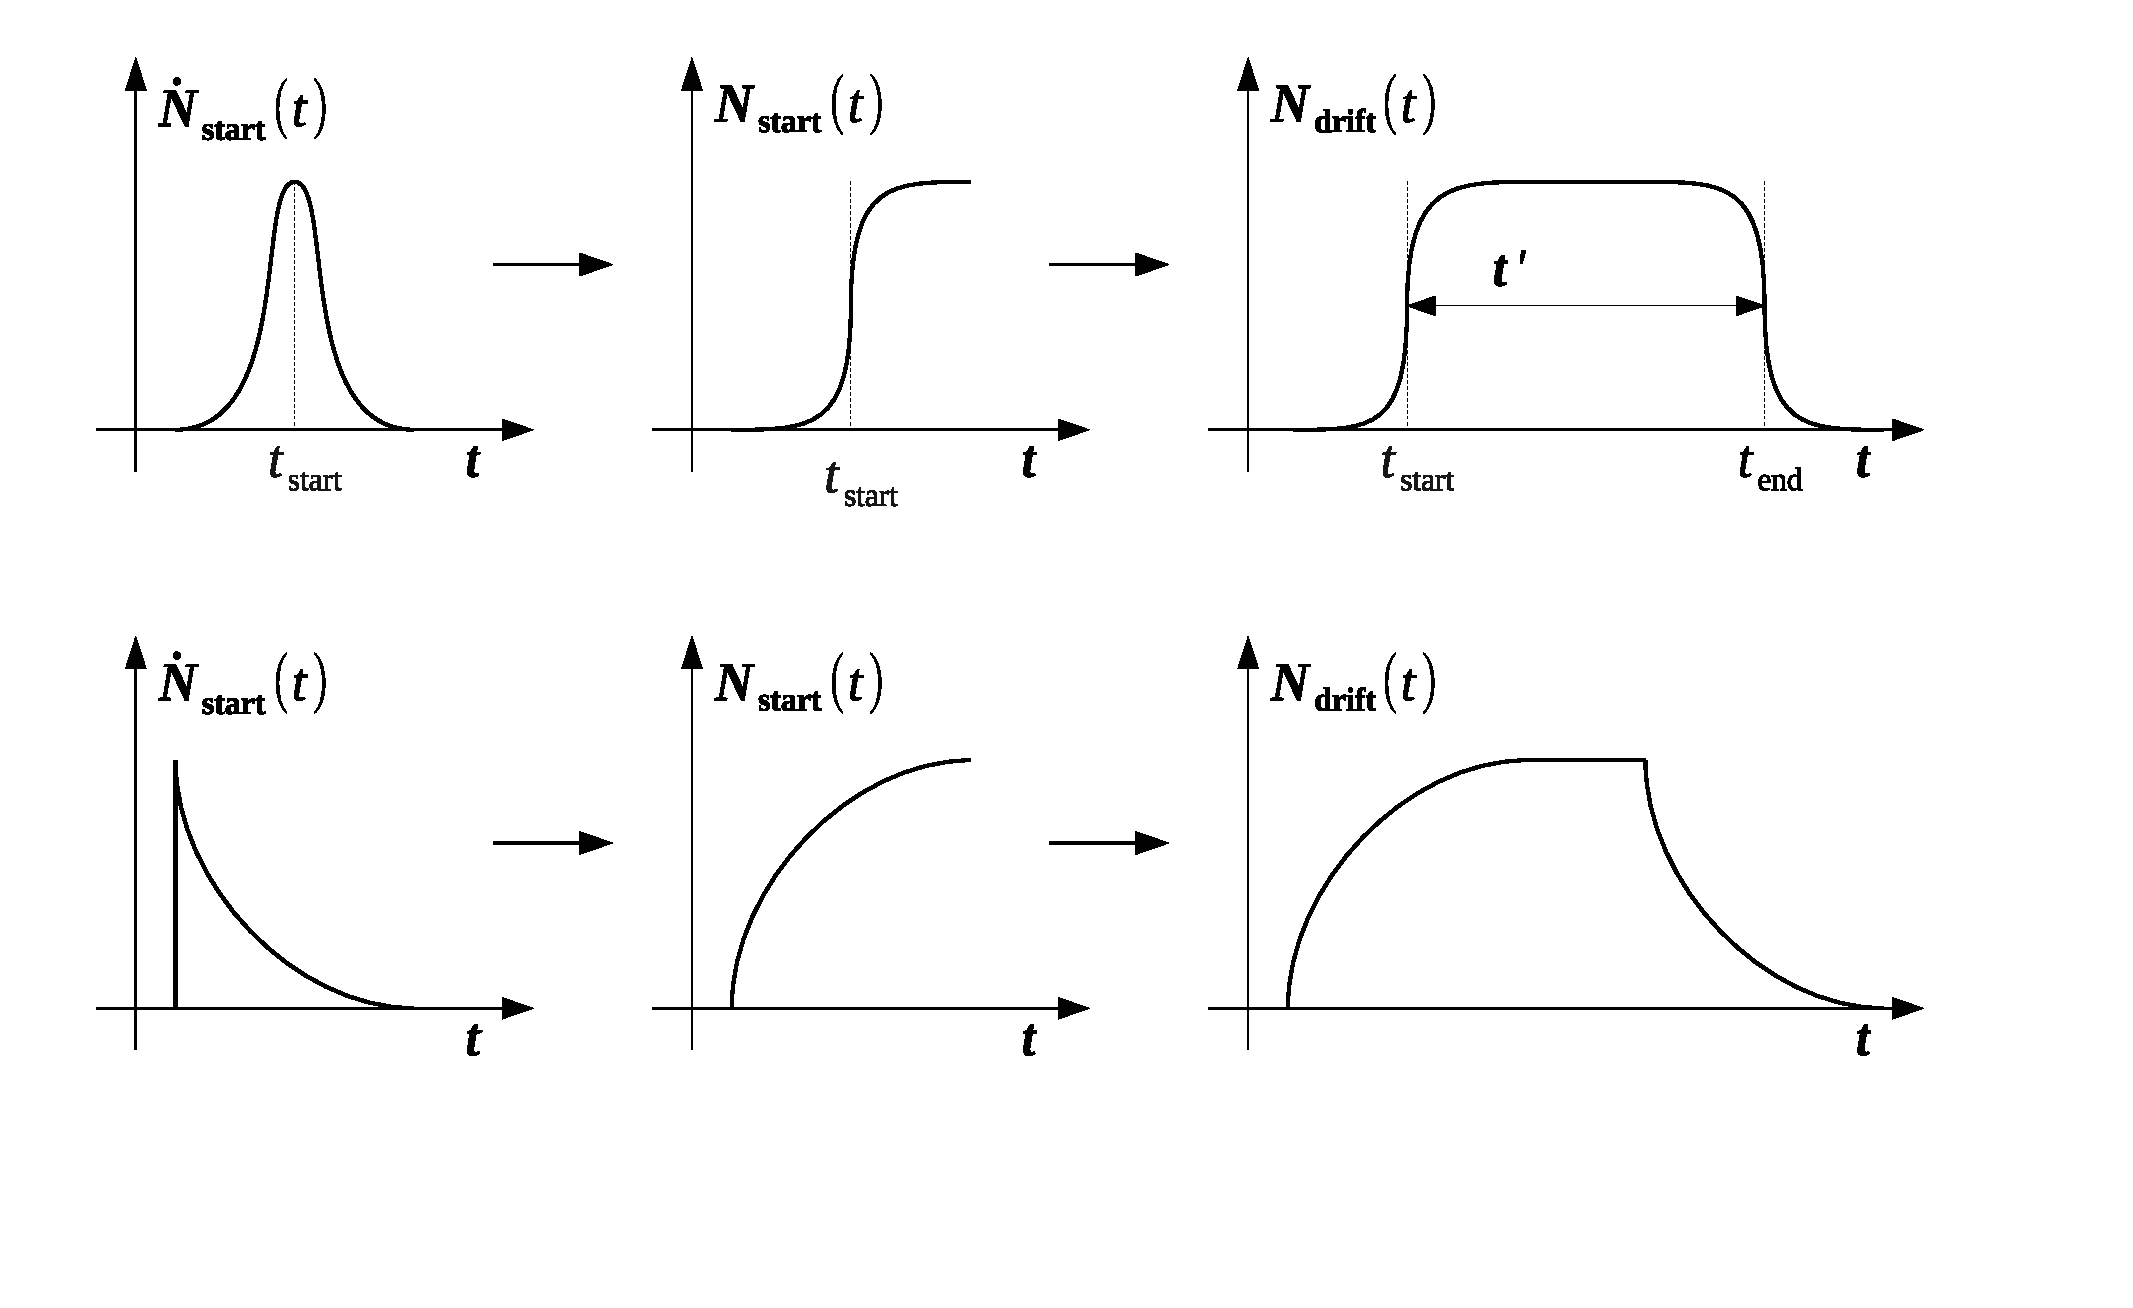
\includegraphics[trim=0cm 3cm 3.5cm 0cm, clip=true,width=0.79\textwidth]{figures/driftingcharges2.eps}
\put(-380,175){(A)}
\put(-380,69){(B)}
 \caption{\textbf{(A)} A Gaussian and \textbf{(B)} an exponential start time distribution function \textbf{(left column)},
 their resulting number of started charges distribution function \textbf{(middle column)}
 and the drifting charges distribution \textbf{(right column)} are shown.}
 \label{fig:collection}
\end{figure}


\subsection{Total integrated current}

\begin{figure}[tb]
 \centering
 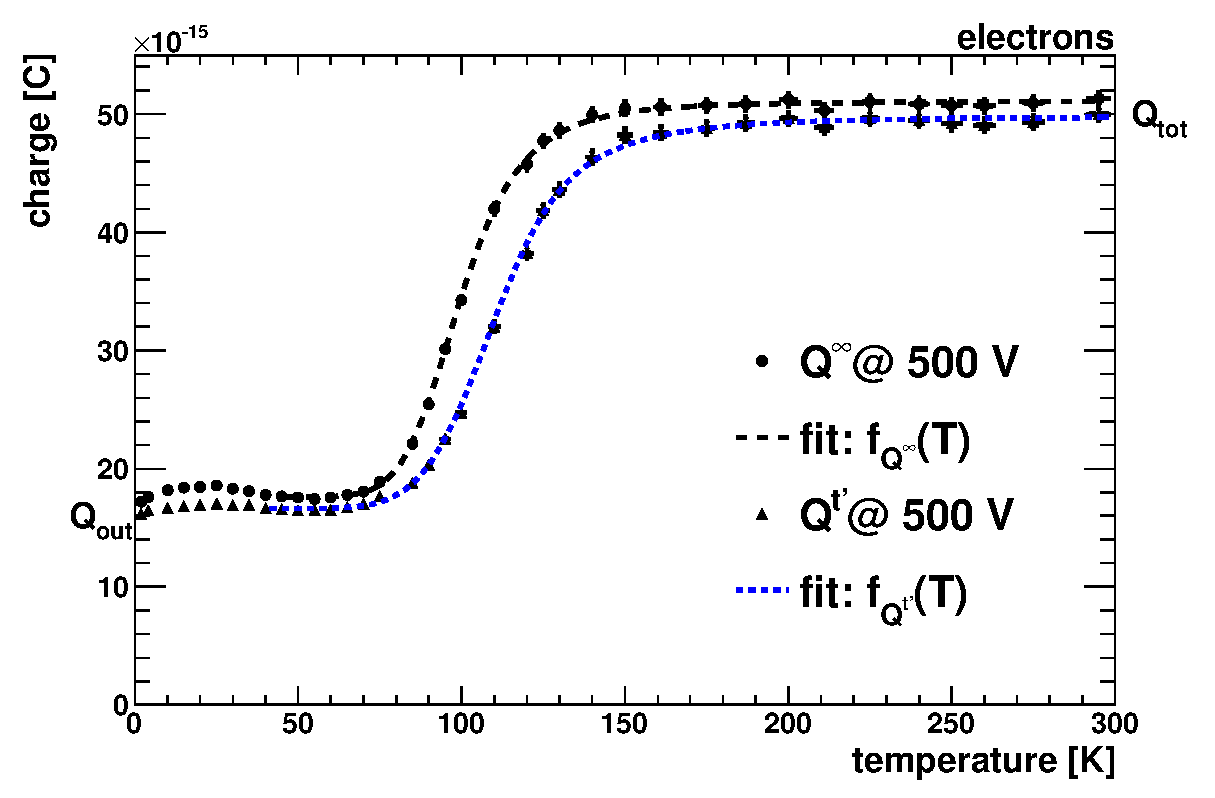
\includegraphics[width=0.49\textwidth]{figures/QttrTmultiE_e.eps}\put(-180,110){\LARGE (A)}\vspace{0.3cm}
 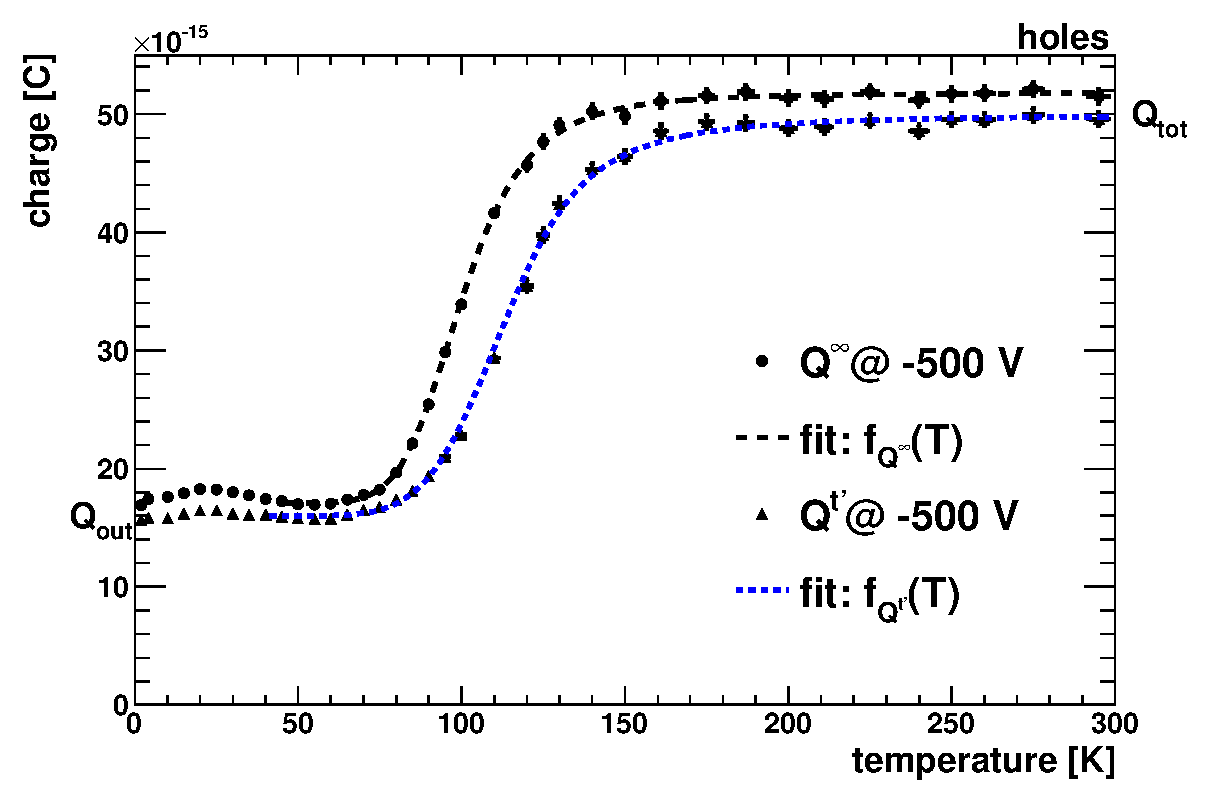
\includegraphics[width=0.49\textwidth]{figures/QttrTmultiE_h.eps}\put(-180,110){\LARGE (B)}
 \caption{The measured charge as a function of the temperature is shown for $Q^{\textrm{|infty}}$ and $Q^{t'}$ for \textbf{(A)} electrons and \textbf{(B)} holes.}
 \label{fig:QT}
\end{figure}

The measured current is integrated over time and analysed as a function of temperature, which is shown in 
 Fig.~\ref{fig:QT} for electrons \textbf{(A)} and holes \textbf{(B)} at $E \approx \SI{1}{\volt/\micro\meter}$, or an applied voltage of $\SI{500}{\volt}$. 
An S-curve describes the overall shape of the measured charge. 
Two variations of the collected charge are shown, the upper one, $Q^{\infty}$, integrates the current including the exponentially falling tail,
 the lower one, $Q^{t'}$ integrates up to the transit time omitting the tails. 
The statistical uncertainty on the charge is estimated to be around 1\,\%. 
The integral of the current pulses is constant at about $Q = \SI{52.0(5)}{\femto\coulomb}$ between room temperature and $\SI{150}{\kelvin}$,
 decreases to about one third of the RT value towards $\sim$ $\SI{75}{\kelvin}$, and remains at this level towards even lower temperatures.
The fit-function, justified in section~\ref{sec:discussion}, contains four parameters: (1) the total charge, (2) the \textit{outer} charge, cf.\ section~4, and (3) a factor $\varepsilon$ in combination with a
 Boltzmann factor 
 with (4) an activation energy $\Ea$. 
The total charge $\Qtot$ and the outer charge $\Qo$ are highly predetermined by the two plateaus before and after the charge drop at about 52\,fC and 17\,fC, respectively, 
 and the inner charge is then $\Qin = \Qtot - \Qo$. 
The fit function for the measured charge $Q^{\infty}$ becomes

\begin{equation}
 f_{Q^{\infty}}(T) = \Qo + \frac{\Qin}{1+\varepsilon\cdot\exppEa},\phantom{\frac{\tau}{\ttr}\exp{\left(-\ttr/\tau\right)}}.
 \label{eq:fitQinfty}
\end{equation}

The fit-function for $Q^{t'}$ is more complicated, as it involves the transit time $\ttr$ and the shape constant $\tau$. 
Therefore, it contains five free parameters ($\Qtot$, $\Qo$, $\varepsilon$, $\Ea$, $\tau$). %, again with $\Qtot$ and $\Qo$ highly predetermined. 
$\ttr$ is taken from data, cf. section~\ref{sec:tt},
 i.e.~a simple power law fit of the transit time as a function of the temperature at $E \approx \SI{1}{\volt/\micro\meter}$. 
The fit-function then reads

\begin{equation}
 f_{Q^{t'}}(T) = \Qo + \frac{\Qin}{1+\varepsilon\cdot\exppEa}\cdot \frac{\tau}{\ttr} \cdot \left[ 1 - \frac{\tau}{\ttr} (1 - \exp{\left(-\ttr/\tau\right)}  ) \right] ,
 \label{eq:fitQtprime}
\end{equation}

\noindent
with a shape constant $\tau$ describing the exponential flanks. 

\begin{table}[tb]
 \centering
 \caption{The results of fitting, firstly, Eq.~(\ref{eq:fitQtprime}) to the charge collected until $\ttr$ ($Q^{t'}$, i.e.~without the tail)
 and secondly Eq.~(\ref{eq:fitQinfty}) to the charge including the tail ($Q^{\infty}$) are listed for electrons and holes at a bias voltage of 500\,V. {\color{red}(A3)}}
   \vspace{0.5cm}

 \begin{tabular}{lcccccc}
\toprule
 & \multicolumn{6}{c}{$Q^{t'}$}  \\  \midrule% \cmidrule(r){2-6} \cmidrule(l){7-10}
 & $\Qtot$\,[fC] & $\Qo$\,[fC] & $t_{e,0}$\,[ps] &  $\taurec$\,[ns]  & $\Ea$\,[meV]& $\chi^2/\textrm{ndf}$\\
% &  fixed	 &  free       & free  &  free     &                             & fixed         & free        & free                           & \\
\midrule
 $\e$ & $\num{49.8(2)}$ & $\num{16.6(3)}$ & $\num{0.6(2)}$ & $\num{14}$ (fixed) & $\num{79(3)}$ & 0.9 \\
 $\h$ & $\num{50.0(2)}$ & $\num{16.0(3)}$ & $\num{1.1(3)}$ & $\num{14}$ (fixed) & $\num{76(3)}$ & 1.4 \\ \midrule
 & \multicolumn{6}{c}{$Q^{\infty}$}\\ \midrule
 & $\Qtot$\,[fC]   & $\Qo$\,[fC]     &  $\num{e5}\,\varepsilon$  & & $\Ea$\,[meV] & $\chi^2/\textrm{ndf}$ \\ 
 \midrule
$\e$ & $\num{51.1(2)}$ & $\num{17.6(3)}$ & $\num{2.8(9)}$     & & $\num{90(3)}$ & 0.4\\
$\h$ & $\num{51.8(2)}$ & $\num{17.1(3)}$ & $\num{5.1(15)}$    & & $\num{85(3)}$ & 0.5\\
avg  & 51.5            & 17.4            & $\num{3.4(8)}$     & & $\num{87.5(22)}$ & \\
\bottomrule
 \end{tabular}
 \label{tab:fitQ}
\end{table} %FIXME re-fit, paste values

{\color{red}(A2)} [The result of the fits for $Q^{t'}$ and $Q^{\infty}$ are tabulated in Tab.~\ref{tab:fitQ} for both carrier types
 and the fit-functions are superimposed as dotted lines in Fig~\ref{fig:QT}. 
The inner charge constitutes about 2/3 of the total charge at a field of $E = \SI{1}{\volt/\micro\meter}$, the outer charge about 1/3,
 summing to a total of about 52\,fC. 
Estimates of $t_{e,0}$ and $\taurec$ are obtained by the following consideration. 
At around 100\,K, $\Qin$ has decreased to half of its RT value, see Fig.~\ref{fig:QT}. 
Therefore $\frac{1}{1+\frac{\tauevap}{\taurec}} = \frac{1}{2}$ and hence $\tauevap = \taurec$. 
With a measured shape constant of $\SI{7}{\ns}$ at 100\,K, cf.\ section~3.5, both the recombination lifetime and the evaporation time at 100\,K are $\sim$ $\SI{14(2)}{\ns}$,
 and therefore $\tauevap = t_{e,0} \exppEa \approx \SI{14}{\ns}$.
Thus, $t_{e,0}$ becomes 

\begin{equation}
 t_{e,0} = \SI{14(2)}{\ns} / \exp{\big( \SI{0.0875}{\eV}/(\kB\cdot \SI{100}{\kelvin}) \big)} = \SI{0.5(1)}{\ps}.
\end{equation}

\noindent
(!) The fit $f_{Q^{t'}}$ does not converge for $\taurec$, we therefore fixed $\taurec$ at a reasonable value of $\taurec = \SI{14}{\ns}$. 
Then, the fit yields
\begin{equation}
 t_{e,0} = \SI{0.6(2)}{ps}
\end{equation}
 
\noindent
in reasonable accordance with the earlier evaluated $t_{e,0}$-value.  
A third estimation results from the $Q^{\infty}$-fit (Eq.~(\ref{eq:fitQinfty})), where only the ratio $\varepsilon = t_{e,0}/\taurec$ appears:
\begin{equation}
 \varepsilon = t_0/\taurec = (\num{3.4(8)})\,\num{e-5}
\end{equation} 

\noindent
averaging the results from electrons and holes, see Tab.~\ref{tab:fitQ}. 
Using again the evaporation time $\tauevap \approx \SI{14(2)}{\ns}$, it is found that

\begin{equation}
 t_{e,0} = \SI{14(2)}{\ns} \cdot \varepsilon = \SI{0.5(2)}{\ps}.
\end{equation}

\noindent
With $t_{e,0} \approx \SI{0.5}{\ps}$, the evaporation time at 50\,K, 150\,K and 300\,K follow to be of the order of $\SI{600}{\micro\second}$, $\SI{600}{\micro\second}$ and $\SI{30}{\ps}$, respectively. 
It is emphasised that the experimentally found scale of $t_{e,0}$ is crucial for the description of the observed data.
If $t_{e,0}$ was of the order of femtoseconds, the charge would not have decreased to half of its RT value at 100\,K, but at 58\,K. 
Also, the rise time of the current pulse at 150\,K would have increased to ??, which is experimentally not observed. 
In the same manner, activation energies of the order of 40\,meV are strictly excluded. 
]

\begin{figure}[tb]
 \centering
 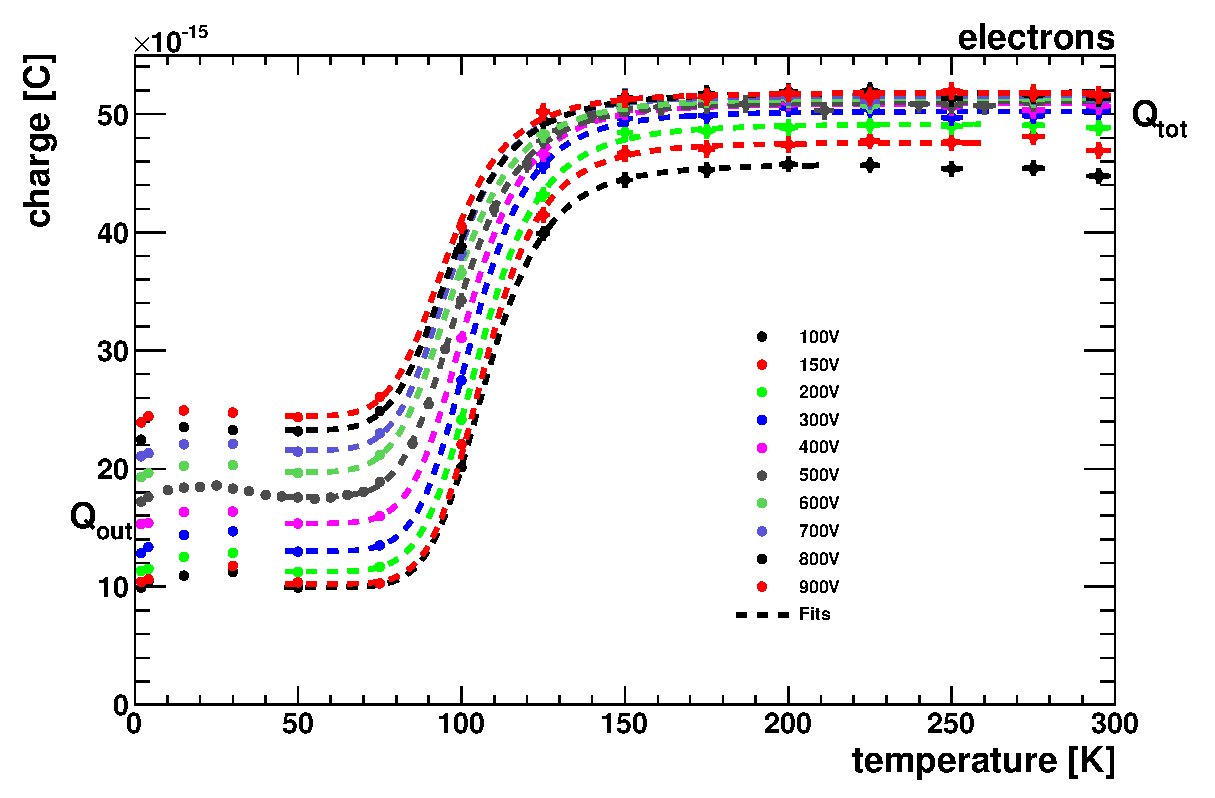
\includegraphics[width=0.49\textwidth]{figures/QTmultiE_e.eps}\put(-180,120){(A)}\vspace{0.3cm}
 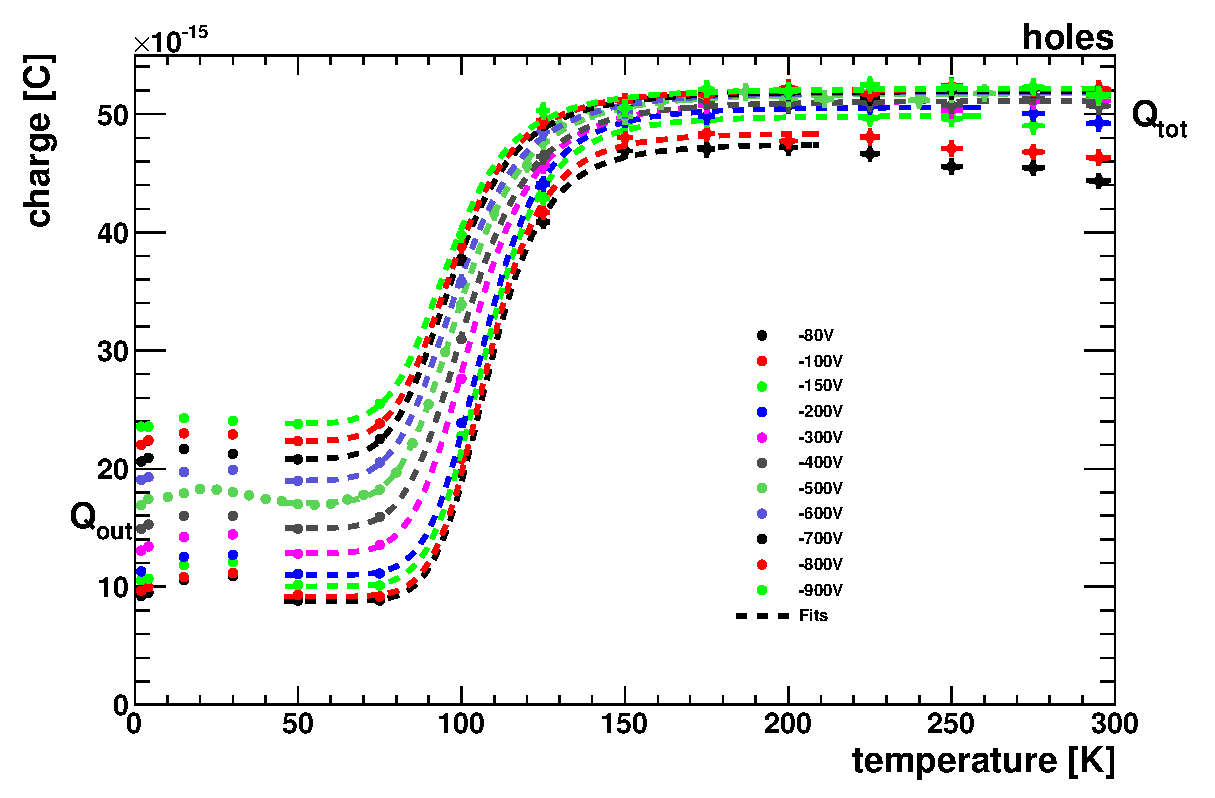
\includegraphics[width=0.49\textwidth]{figures/QTmultiE_h.eps}\put(-180,120){(B)}
 \caption{The measured charge $Q^{\infty}$ as a function of the temperature is shown for various voltages for electrons \textbf{(A)} and holes \textbf{(B)}.}
 \label{fig:QTvoltage}
\end{figure}

The S-curves for different voltages are shown for $Q^{\infty}$ in Fig.~\ref{fig:QTvoltage}. 
Again, the similarity between electron and hole pulses is evident. 
The fit described earlier is performed for charge data from 100\,V to 900\,V, each fit resulting in a value for $\varepsilon$, and $\Ea$. 
The discussion of the temperature dependence of the fit-parameters ist postponed to section~\ref{sec:discussion}. 

\begin{figure}[tb]
 \centering
 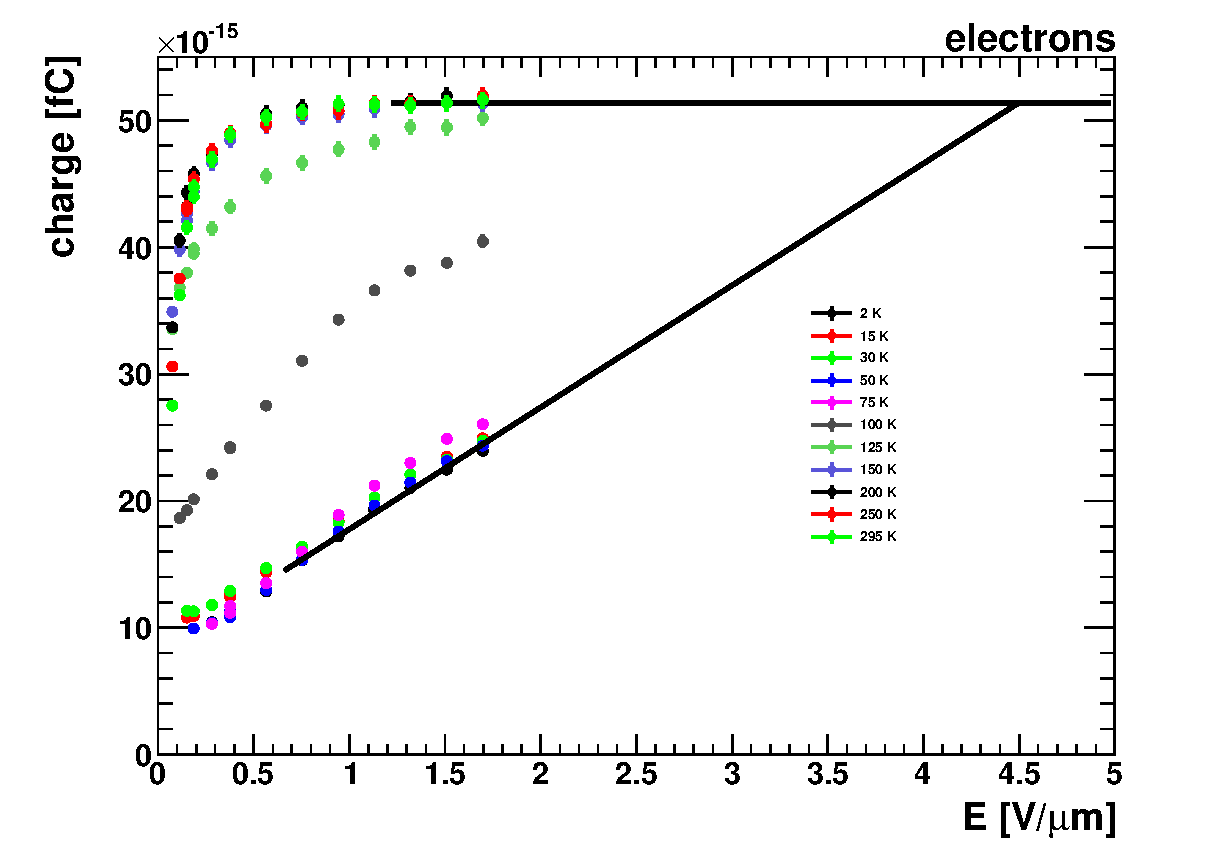
\includegraphics[width=0.49\textwidth]{figures/QEmulti_e}\put(-180,120){(A)}\vspace{0.3cm}
 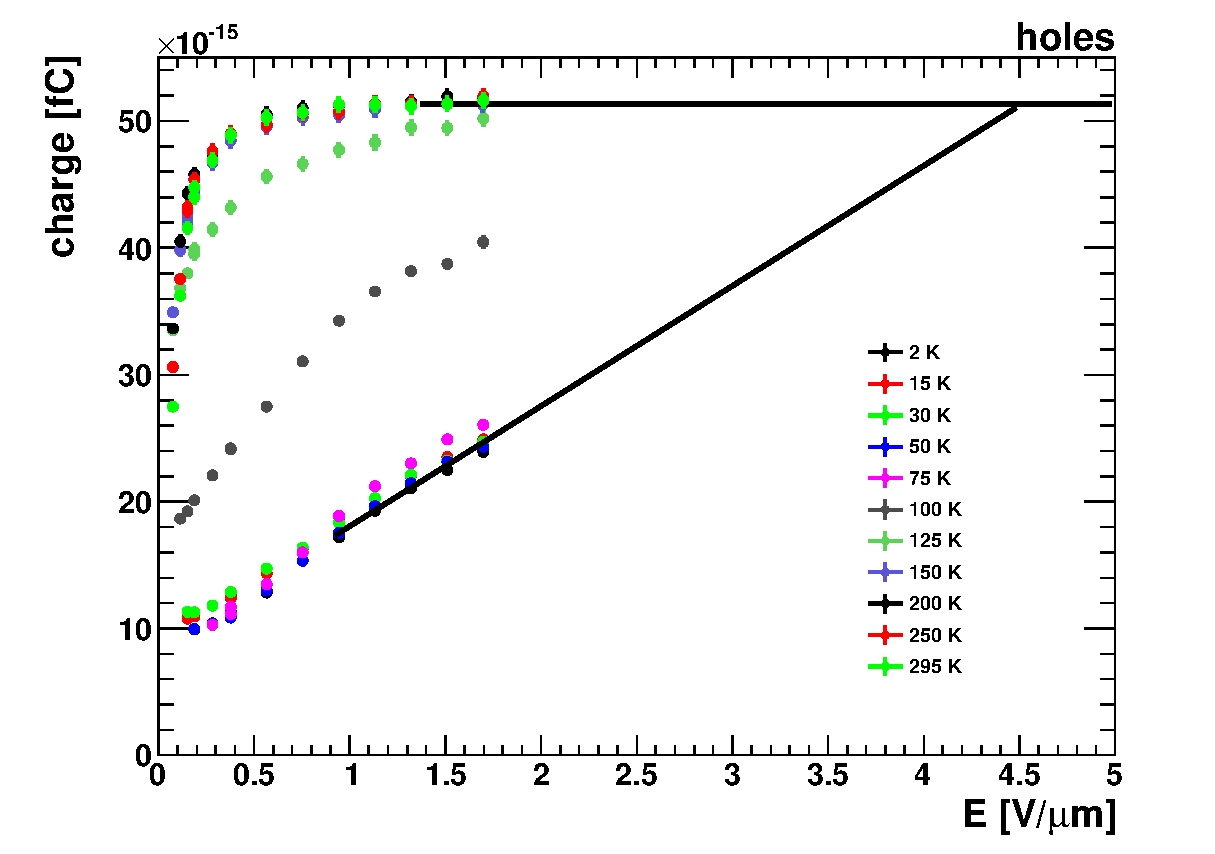
\includegraphics[width=0.49\textwidth]{figures/QEmulti_h}\put(-180,120){(B)}
 \caption{The measured charge $Q^{\infty}$ as a function of the applied field strength is shown for various temperatures for electrons \textbf{(A)} and holes \textbf{(B)}.}
 \label{fig:QvsE}
\end{figure}

Plotted as a function of the electric field strength, the influence of the field on the measured charge becomes evident.
Figure~\ref{fig:QvsE} shows the same behaviour for all temperatures above 150\,K, and below 75\,K. 
The first increases rapidly with field strength and reaches a flat top at about $\SI{1}{\volt/\micro\meter}$, whereas the latter increases linearly. 
The discussion of this behaviour is covered in section~4. 

\subsection{Fit-function for the current pulses}

The transit time and characteristic time constant are determined by the time difference between end time and start time of drift,
 $t_{\text{e}}$ and $t_{\text{s}}$ respectively, hence $\ttr = t_{\text{e}} - t_{\text{s}}$.
A function $f(t;P)$ is fitted to each current pulse in order to find $t_{\text{e}}$ and $t_{\text{s}}$.
$f(t;P)$ is a function of time and a set of parameters $P$ incorporating two complementary error functions $(2-\Erfc(t-t_{\text{s}}))$ and $\Erfc(t-t_{\text{e}})$
 describing the rising and the falling edge, respectively. 
Additionally, an exponential component  of the form $\left( 1-\exp \left(-(t-t_{\text{s}})/\tau\right) \right) - \Theta_{\textrm{col}}(t;t_{\text{e}})$ with
  $\Theta_{\textrm{col}}(t;t_{\text{e}}) = 1 - \exp \left( -(t-t_{\text{e}})/\tau \right)$ for $t > t_{\text{e}}$ and $\Theta_{\textrm{col}}(t;t_{\text{e}}) = 0$ otherwise,
 is allowed, cf.~Eq.~(\ref{eq:collection}). 
The error functions describe a Gaussian probability distribution for the start time of the drift around $t_{\text{s}}$,
 and respectively a collection at the opposite electrode around $t_{\text{e}}$. 
The 50\% points mark $t_{\text{s}}$ and $t_{\text{e}}$, respectively. 
The fit parameter $\tau$ is given a physical meaning in the discussion section. 

At all temperatures and fields, the fit-function describes well the measured pulse shape of $i_m(t)$;
 each fit resulting in a value for $\tau(T,E)$ and $\ttrans(E,T)$.
One example of a fit to a measured pulse $i_m(t)$ at 100\,K and 500\,V is shown in Fig.~\ref{fig:ExModel2}. 
The resulting shape constant is $\tau(\SI{100}{\kelvin},\,\SI{500}{\volt}) \approx (\num{6.8}\pm\num{0.1}_{\textrm{stat}}\pm\num{1.0}_{\textrm{sys}})\,\si{\ns} \approx \SI{7(1)}{\ns}$. 
The current induced from charges stemming from the outer and the inner part of the cloud are shown separately as dashed lines
 featuring the error-function shape and the exponential shape, respectively.
The sum forms the solid line on top of the data. 
At this temperature, a certain fraction of the charge recombines. 

\subsection{Characteristic time constant}

\begin{figure}[t]
 \centering
 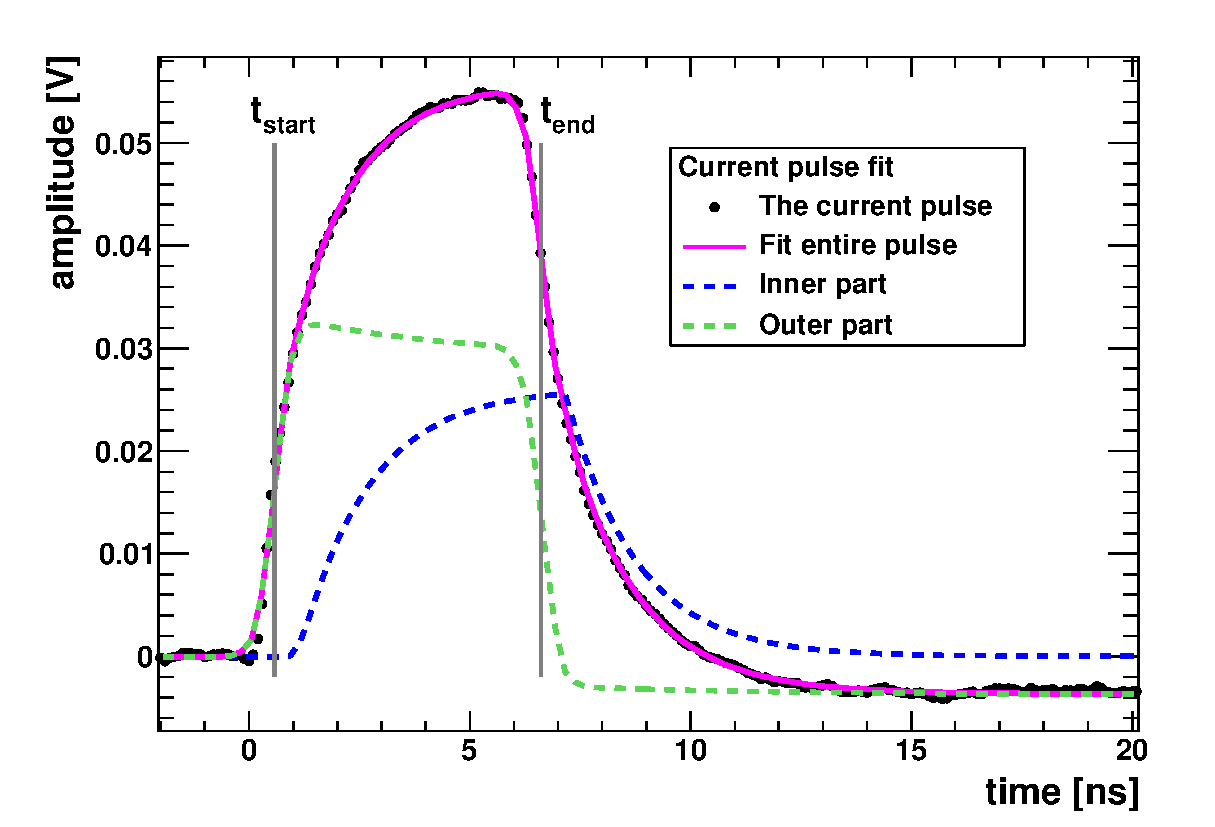
\includegraphics[width=0.59\textwidth]{figures/ex_pulsefit3}%pulseFit.C
 \caption{The fit to the measured pulse at 100\,K and 500\,V and its components are depicted.}
 \label{fig:ExModel2}
\end{figure}


The fitted shape constant $\tau$ is shown in Fig.~\ref{fig:fittau}
 as a function of temperature (closed circles) at $E \approx \SI{1}{\volt/\micro\meter}$. 
The error bars are the statistical errors resulting from the fit. 
For both electrons and holes $\tau$ remains about constant at $\SI{0.4}{\ns}$ between RT and $\SI{150}{\kelvin}$. 
Between $\SI{150}{\kelvin}$ and $\SI{90}{\kelvin}$, the shape constant increases steeply.%
\footnote{A comparison to measured values in the literature is difficult, or impossible,
 as no measurement of exciton properties in diamond using electric fields are known to the authors.}
Due to the decrease of the amplitude of the tail in the current pulses with decreasing temperature, the signal-to-noise ratio at $T \leq \SI{90}{\kelvin}$
 is too small in order to accurately fit the shape constant. 
The fitted $\tau$ therefore decreases for $T < \SI{90}{\kelvin}$. 
The corresponding region is marked as `insensitive'. 

\begin{figure}[t]
 \centering
  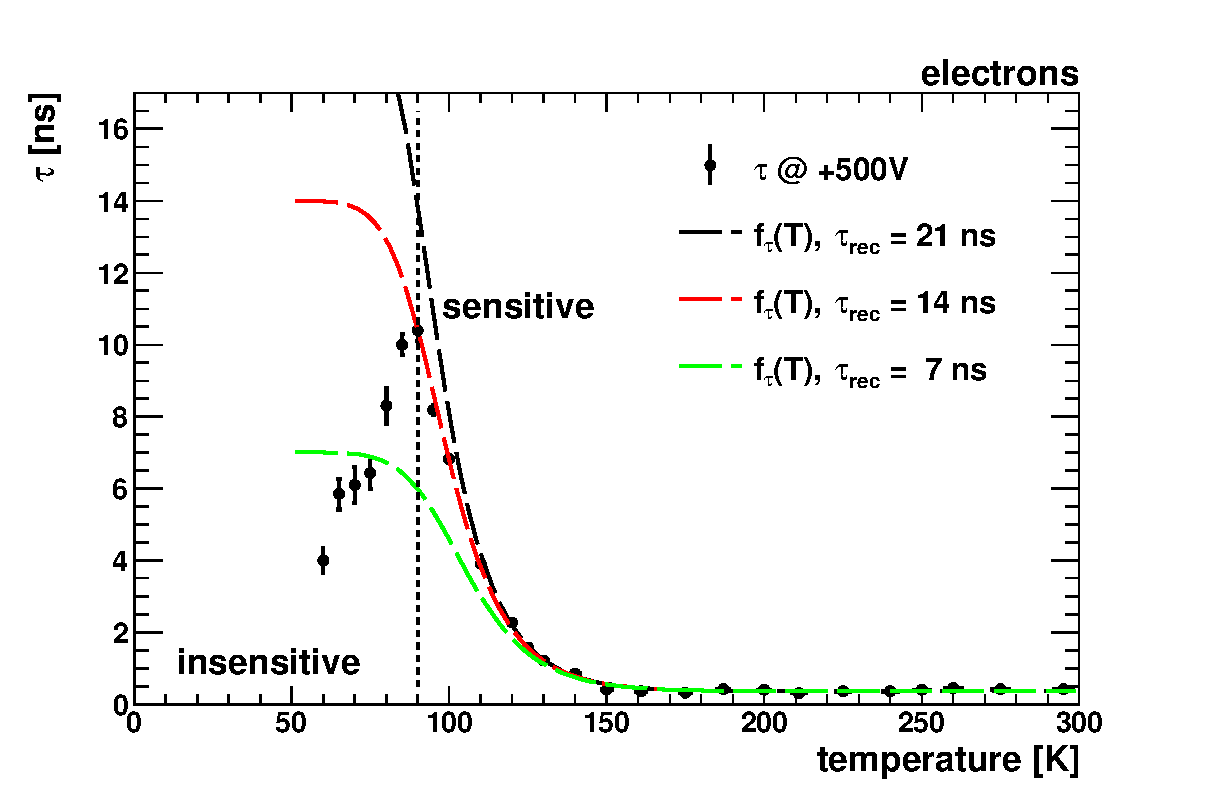
\includegraphics[width=0.49\textwidth]{figures/tauvsT_e}\put(-190,110){(A)}
  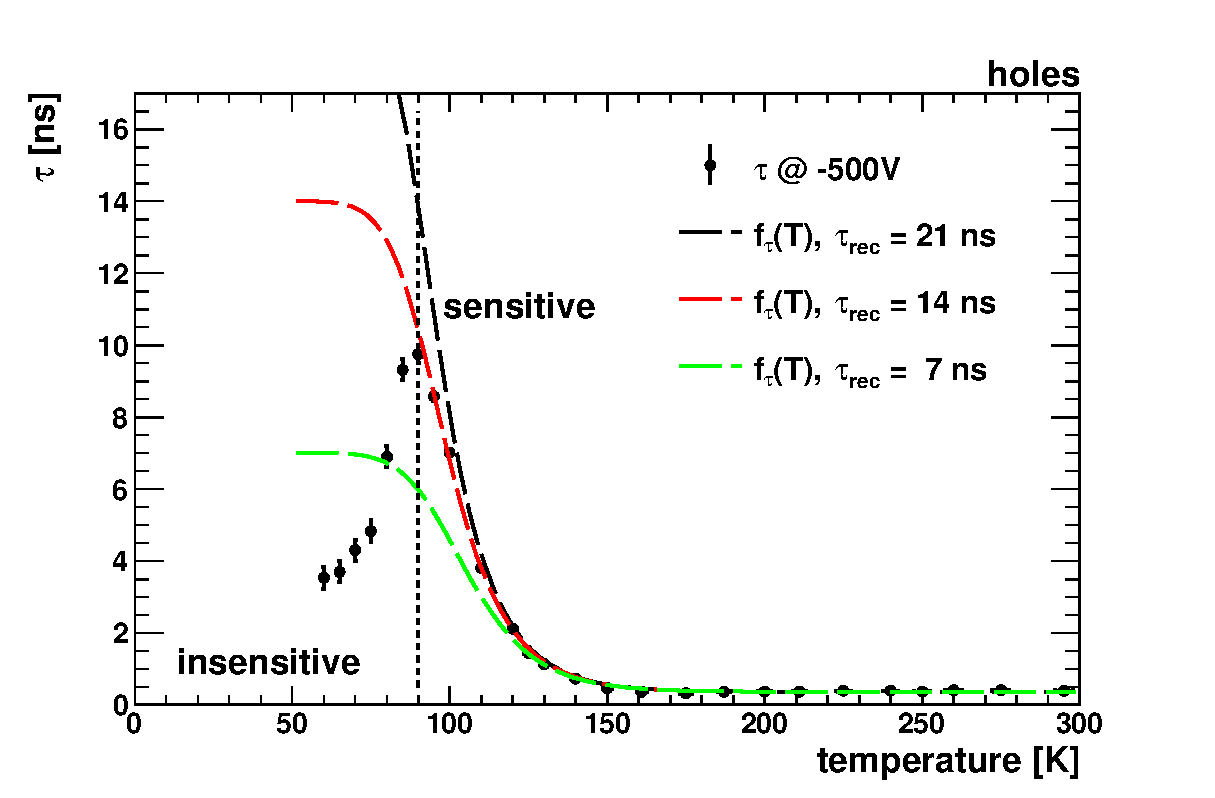
\includegraphics[width=0.49\textwidth]{figures/tauvsT_h}\put(-190,110){(B)}\\
  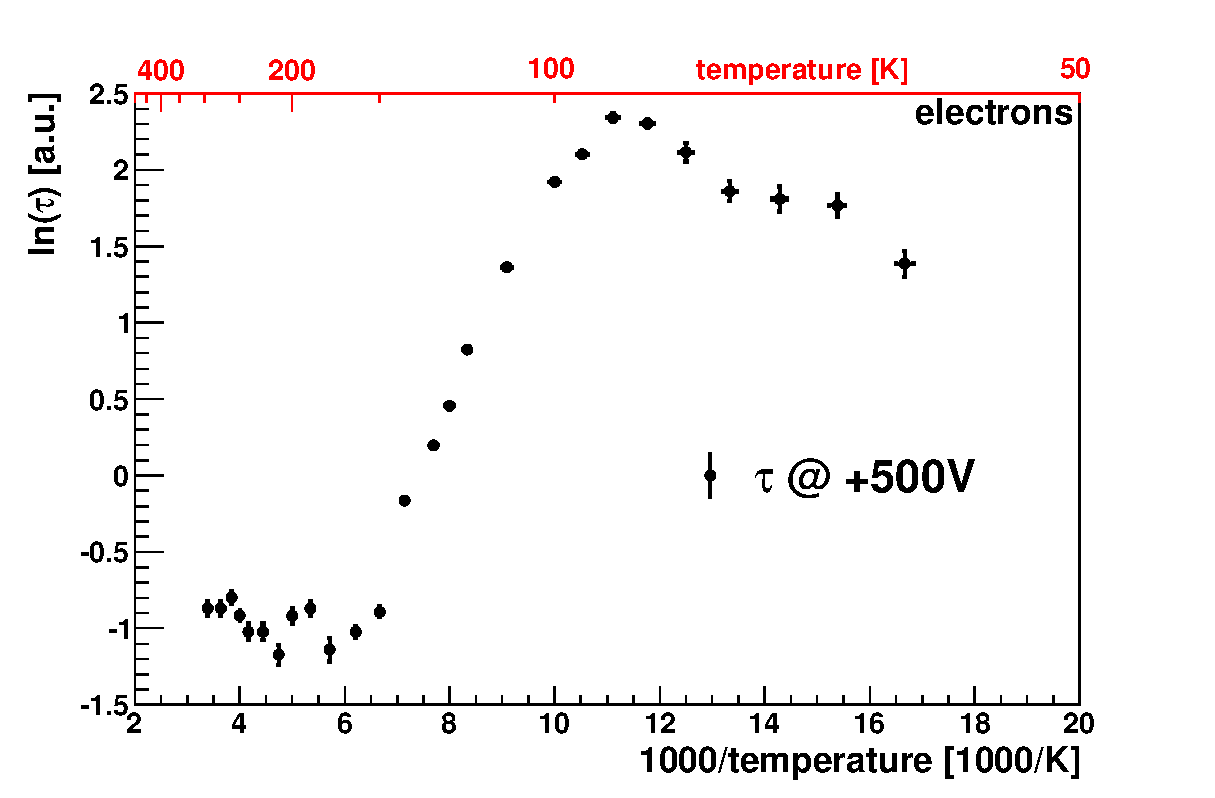
\includegraphics[width=0.49\textwidth]{figures/logtauvsTinv_e}\put(-190,110){(C)}
  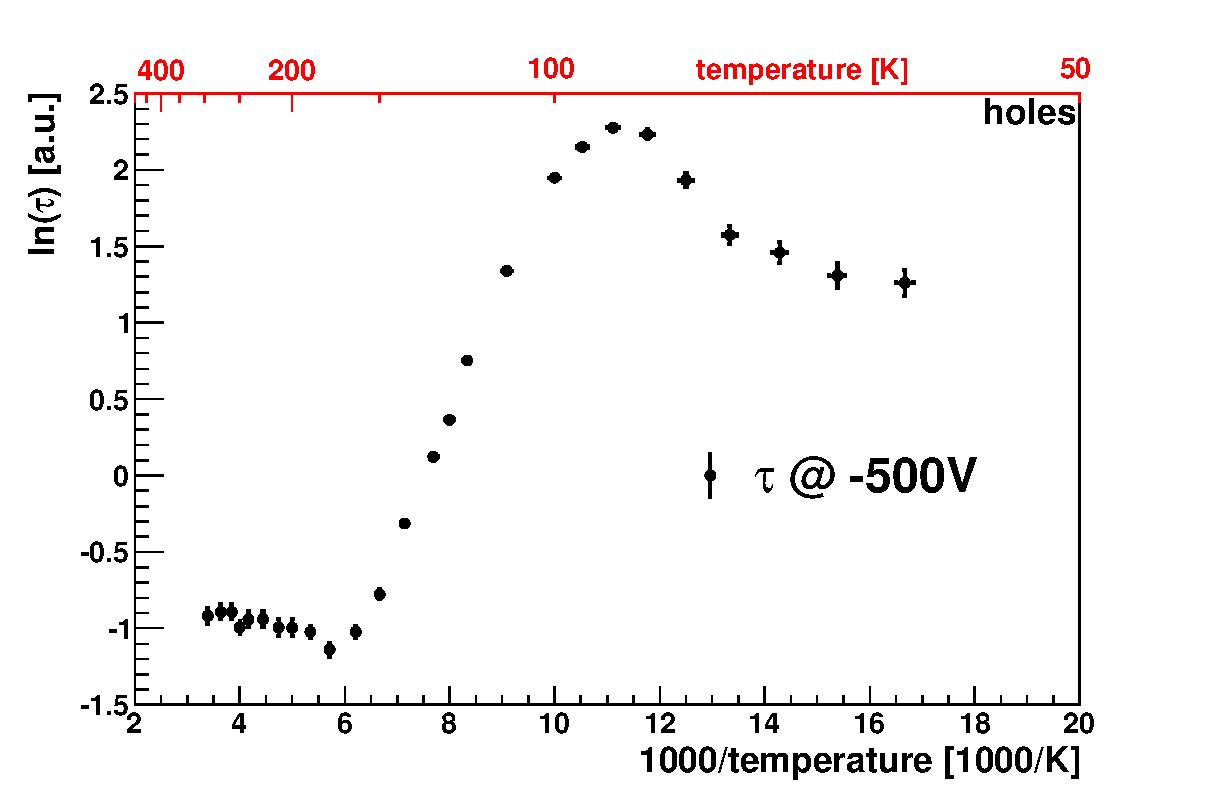
\includegraphics[width=0.49\textwidth]{figures/logtauvsTinv_h}\put(-190,110){(D)}
 \caption{The fitted shape constant $\tau$ is shown as a function of the temperature for electrons \textbf{(A)} and holes \textbf{(B)} at $500$\,V.
\textbf{(C)} and \textbf{(D)} show the results in $\ln{(\tau)}$ vs.~the inverse temperature.}
 \label{fig:fittau}
\end{figure} %FIXME title x-axis = 1000/temperature

We revise, if the measured temperature dependence of $\tau$ can be explained within the exciton model
 using the $t_{e,0}$-value (0.5\,ps) extracted from charge data. 
Using $\frac{1}{\tauzero} =  \frac{1}{\taurec} + \frac{1}{\tauevap}$ and $\tauevap = t_{e,0} \exppEx$ one finds

\begin{equation}
 \tauzero(T) = \left( \frac{1}{\taurec} + \frac{1}{\tauevap(T)} \right)^{-1} = \left( \frac{1}{\taurec} + \frac{1}{t_{e,0} \exppEx }\right)^{-1}.
 \label{eq:tauT}
\end{equation}

\noindent
A possible temperature dependence of the recombination lifetime is not allowed for. 
It is further important to notice that
 the fitted shape constant cannot be faster than the cut-off time constant, which arises from the cut-off frequency of the measuring system. 
In fact, the cut-off constant adds quadratically to the physical shape constant, resulting in the fitted shape constant.
Using Eq.~(\ref{eq:tauT}) and an additional such parameter $\tau_{cut}$, a function $f_{\tau}(T)$ is defined  as

\begin{equation}
 f_{\tau}(T) = \sqrt{\left( \frac{1}{\taurec} + \frac{1}{t_{e,0} \exppEx }\right)^{-2} + \left( \tau_{\textrm{cut}}\right)^2},
 \label{eq:fittau}
\end{equation}

\noindent
which is to be checked against the data. 
Superimposed in Fig.~\ref{fig:fittau} as dashed lines are $f_{\tau}(T)$ with the activation energy $\Ea = \SI{87.5}{\milli\eV}$, $t_{e,0} = \SI{0.5}{\ps}$,
 and three different $\taurec = 7,14,\SI{21}{\nano\second}$. 
It is clear from Fig.~\ref{fig:fittau} that Eq.~(\ref{eq:fittau}) describes the experimental data reasonably well
 using the afore mentioned $\Ea(\SI{500}{\volt}) = \SI{87.5}{\milli\eV}$, $t_{e,0} = \SI{0.5}{\ps}$, and $\taurec = \SI{14}{\ns}$. 
Therefore, a combination of values $\Ex$ and $t_{e,0}$ exists that consistently explains two important parts of the data,
 i.e.~the temperature dependence of both the measured charge and the fitted shape. 

The characteristic time constant shall also be studied as a function of the temperature in order to extract the activation energy as a function of the electric field. 

\begin{figure}[t]
 \centering
  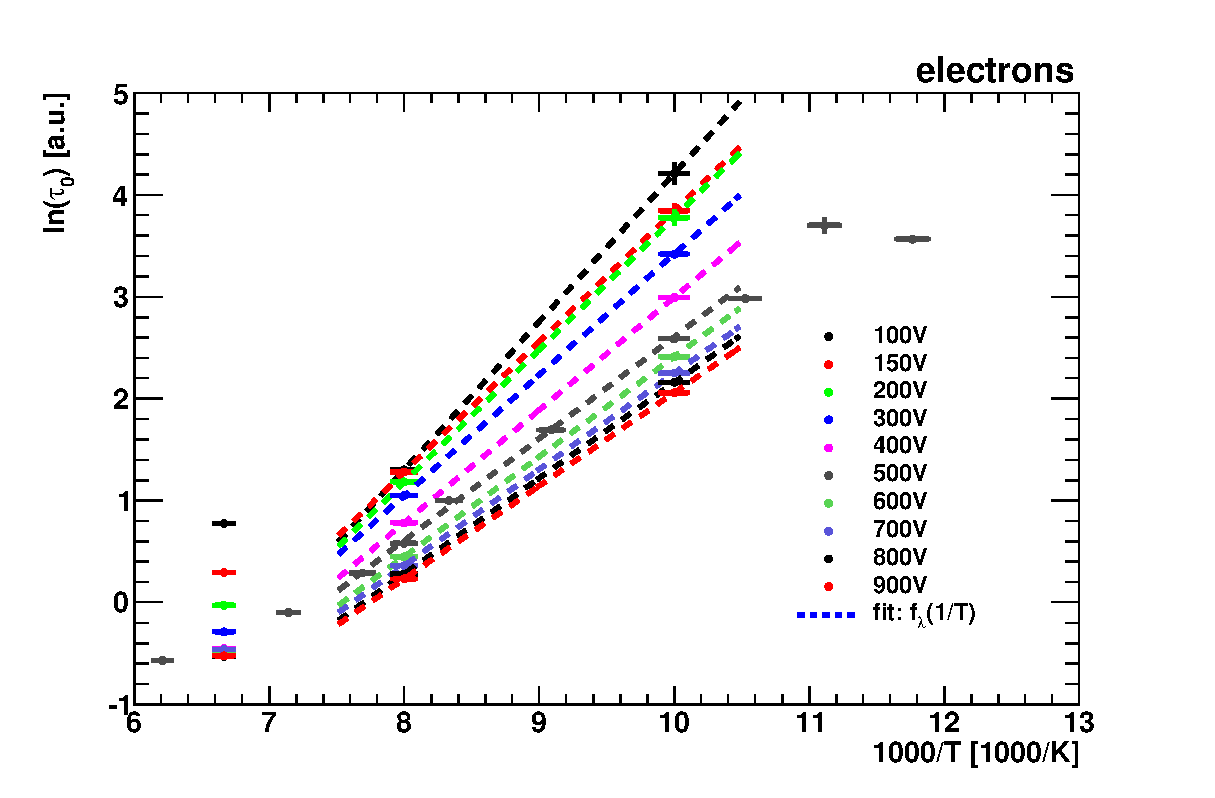
\includegraphics[width=0.49\textwidth]{figures/logtauvsTinvU_e}\put(-190,110){(A)}
  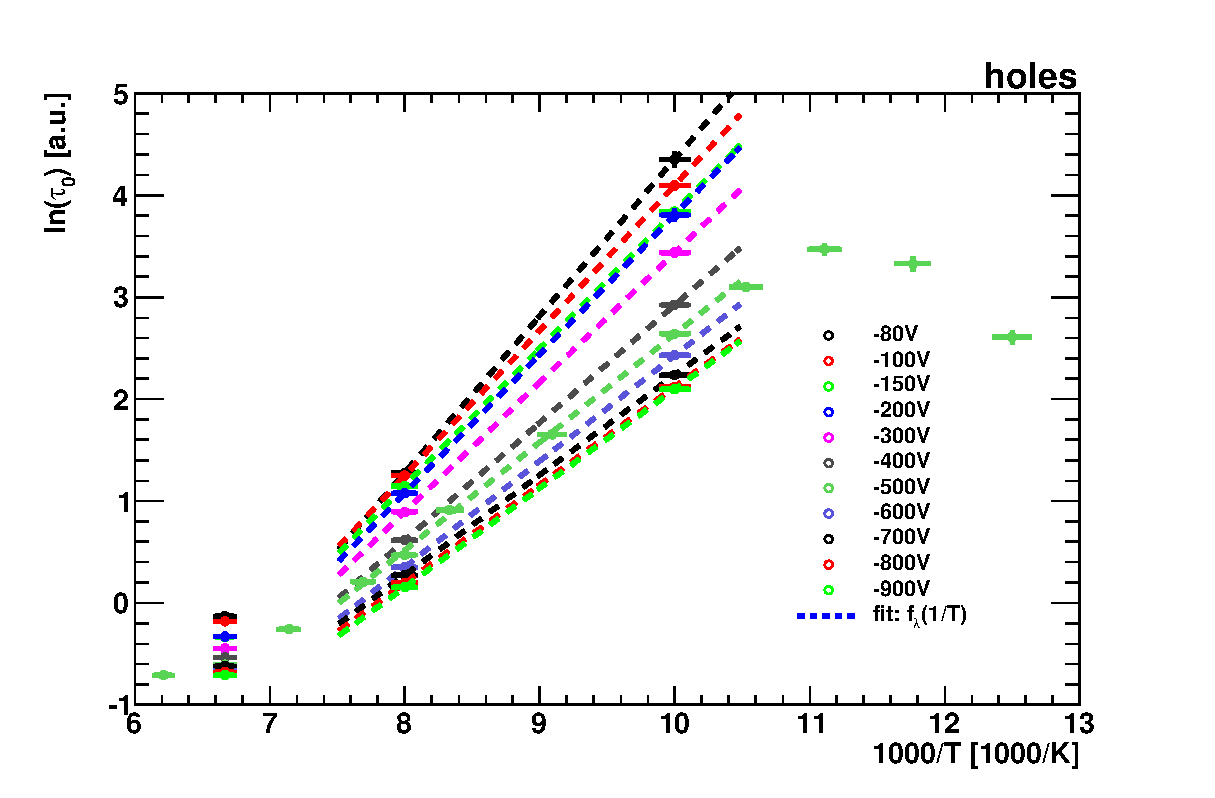
\includegraphics[width=0.49\textwidth]{figures/logtauvsTinvU_h}\put(-190,110){(B)}
 \caption{The fitted shape constant is shown as $\ln{(\tauzero)}$ versus the inverse temperature for various voltages including their corresponding linear fits extracting the activation energy. }
 \label{fig:fittauV}
\end{figure}

\subsection{Transit time}
\label{sec:tt}

\begin{figure}[t]
 \centering
 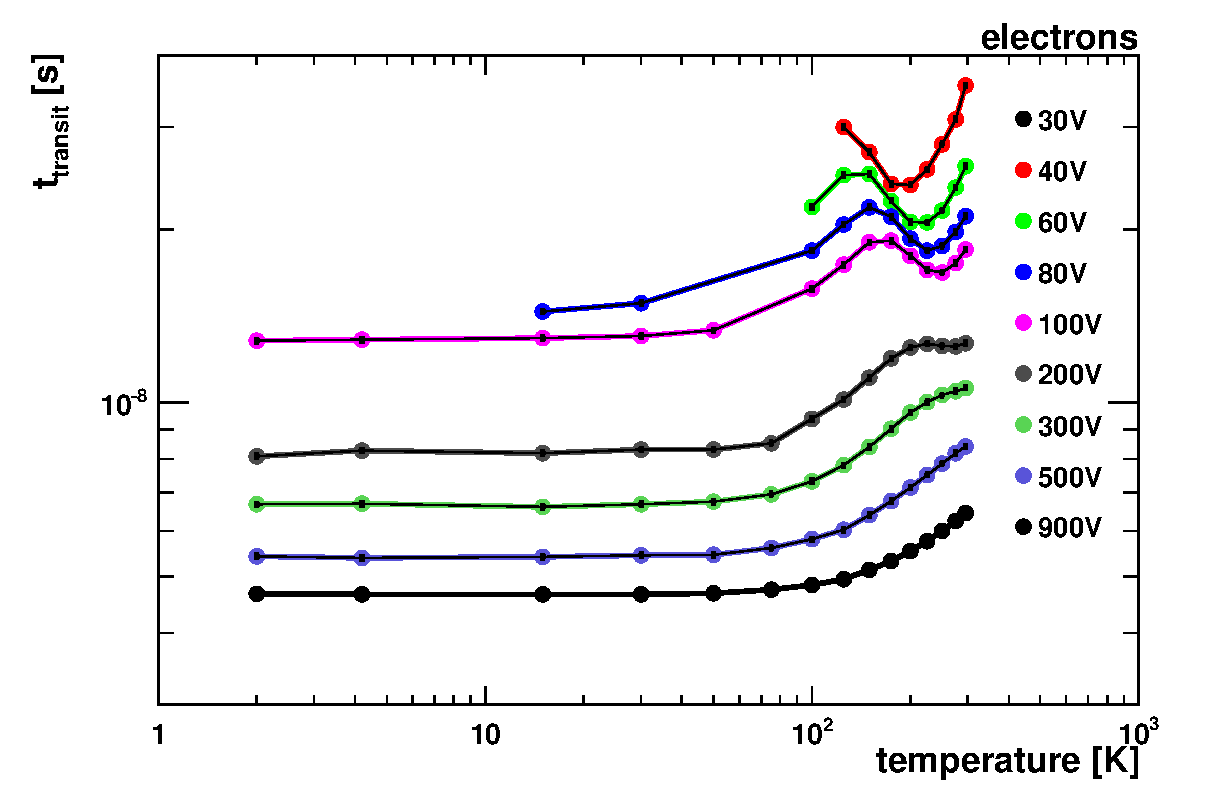
\includegraphics[width=0.49\textwidth]{figures/ttloglog_e.eps}\put(-190,110){(A)}
 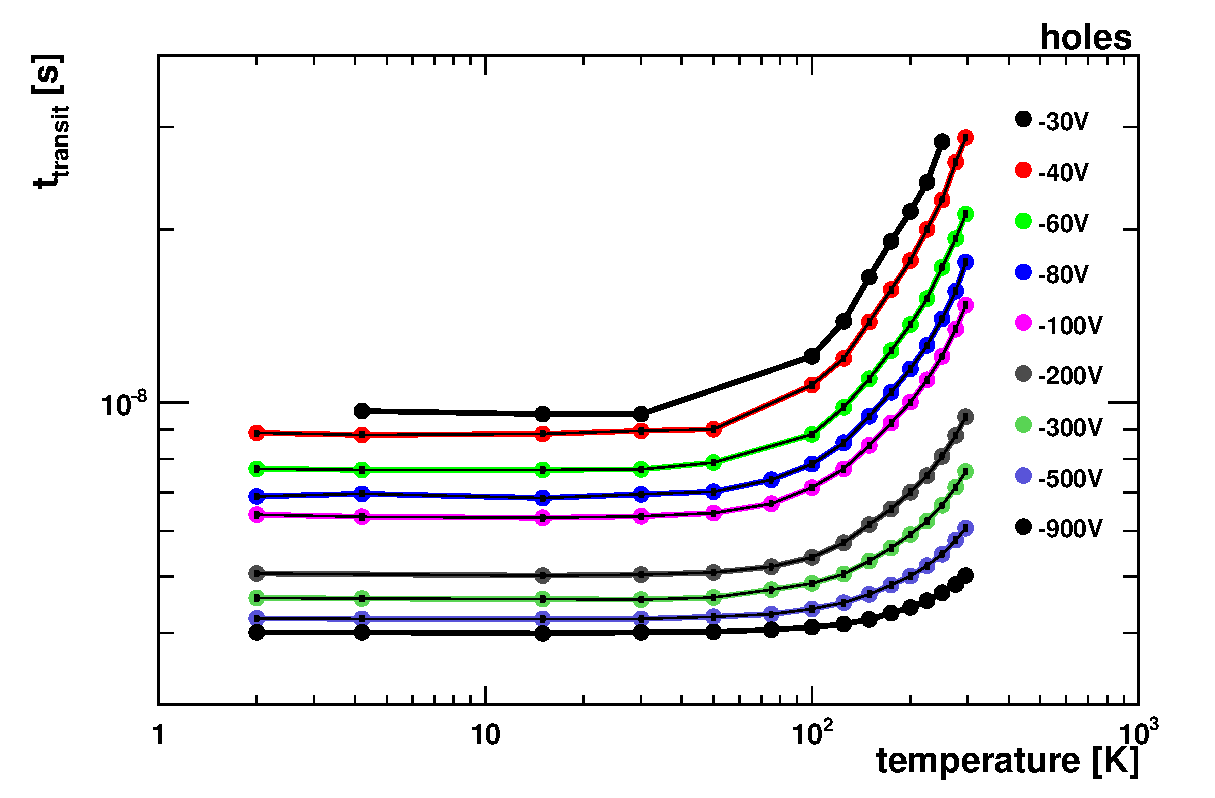
\includegraphics[width=0.49\textwidth]{figures/ttloglog_h.eps}\put(-190,110){(B)}
 

 \caption{The transit times for holes \textbf{(a)} and electrons \textbf{(b)} at various temperatures and fields are shown for \textit{S57}. 
Note the double logarithmic scale. Lines are drawn between measurements for constant voltages in order to guide the eye.}
 \label{fig:tt}
\end{figure}

The measured transit times are shown in Fig.~\ref{fig:tt} for \textit{S57} as an example. 
All three samples show the same behaviour. 
Transit times range from $\SI{3}{\nano\second}$ to $\SI{40}{\nano\second}$ for all fields and temperatures. 
Experimental sources of uncertainties affecting the measurement of the drift velocity are listed below including an estimate of their values.
\begin{itemize}
 \item[1)] The sample thickness has been measured with precision tools resulting in an uncertainty of the sample thickness below $<1\%$.
 \item[2)] The error in the measurement of the transit time $\sigma_{\ttr}$ depends on the ability to identify the rising and the falling edge, which in turn correlates with the SNR.
The SNR depends on the temperature and the electric field. 
$\sigma_{\ttr}$ is estimated as $\sigma_{\ttr} = \frac{\sigma_{\textrm{noise}}}{\textrm{slope}}$, with the baseline noise $sigma_{\textrm{noise}}$ and the maximum slope in the rising edge. 
At room temperature (low temperature) and $E\approx \SI{1}{\volt/\micro\meter}$, this approach leads to uncertainties of the transit time measurement of around $1\%$ ($2\%$),
 and up to $4\%$ at low temperature and low fields.
 \item[3)] At low SNRs the bandwidth limit was used in order to extent the accessible measurement range towards lower electric fields. 
The bandwidth limit leads to slower rising and falling edges. 
The effect on the transit time at $V_{\textrm{bias}} = \SI{100}{\volt}$ at RT is $\approx1\,\%$. 
At lower biases the rising/falling edges are slower, hence the effect is smaller. 
 \item[4)] Errors due to a possible non-uniformity of the electric field can be neglected, as a net-space charge seems to be absent in the tested samples.
 \item[5)] The uncertainty of the electric field strength is conservatively estimated to $1\%$.
 \item[6)] The uncertainty of the temperature measurement is about $1\%$. 
\end{itemize}




Figure~\ref{fig:tt} (a) shows how the transit time for holes increases with temperature over the entire temperature range,
 and how it decreases with increasing field over the whole field range. 
For electrons, Fig.~\ref{fig:tt} (b), the transit time decreases with increasing field, but does not monotonically increase for all biases. 
Only at high biases, down to $\SI{300}{\volt}$, the transit time increases with increasing temperature over the whole temperature range.
For smaller biases, a local maximum emerges, being more pronounced with decreasing bias.
The position of the local maximum shifts to lower temperatures with decreasing bias.
The abnormal behaviour of the electron transit time is likely to be caused by a re-population effect, a well-understood phenomenon in silicon \cite{Jacoboni197777}.
It was recently observed in high-purity scCVD diamond \cite{isberg:172103}, but at much lower temperatures and fields. 

 

\else

\subsection{Initial density estimation}

The impinging $\alpha$-particles create free charge carriers within a small volume of the diamond bulk. 
The ionisation volume is described by the penetration depth of the $\alpha$-particle and its radial size. 
An average penetration depth of $\dpen \approx \SI{10}{\micro\meter}$ is calculated making use of NIST data
 and the radial $1/e$ size is estimated to be $r_0 \approx \SI{2}{\nm}$. 
The short $r_0$ is a result of the amount of energy transferred from the primary $\alpha$-particle to the electrons, 
 which is of the order of 60\,eV, cf.\ \cite{JansenThesis}, section 3.1.1. 
The aspect ratio of the ionisation volume is roughly $\num{10000}/\num{2} = \num{5000}$. 
As is shown later, the amount of charge produced at room temperature is about $Q = \SI{52}{\femto\coulomb}$,
 matching an estimate of an $\alpha$-particle with $\SI{4.3}{\mega\eV}$ at an electron-hole-pair creation energy of $\SI{13.25}{\eV}$. 
The average charge density in the first radial $1/e$ length of the charge cloud in the instant of the impingement is hence estimated as 

\begin{equation}
 n = \frac{0.68\cdot\SI{52}{\femto\coulomb}}{r_0^2\pi \dpen} \approx \SI{5e21}{\pairs/\cm^{3}}.
\end{equation}

\subsection{Induced current pulses from carrier drift}
\begin{figure}[tb]
 \centering
 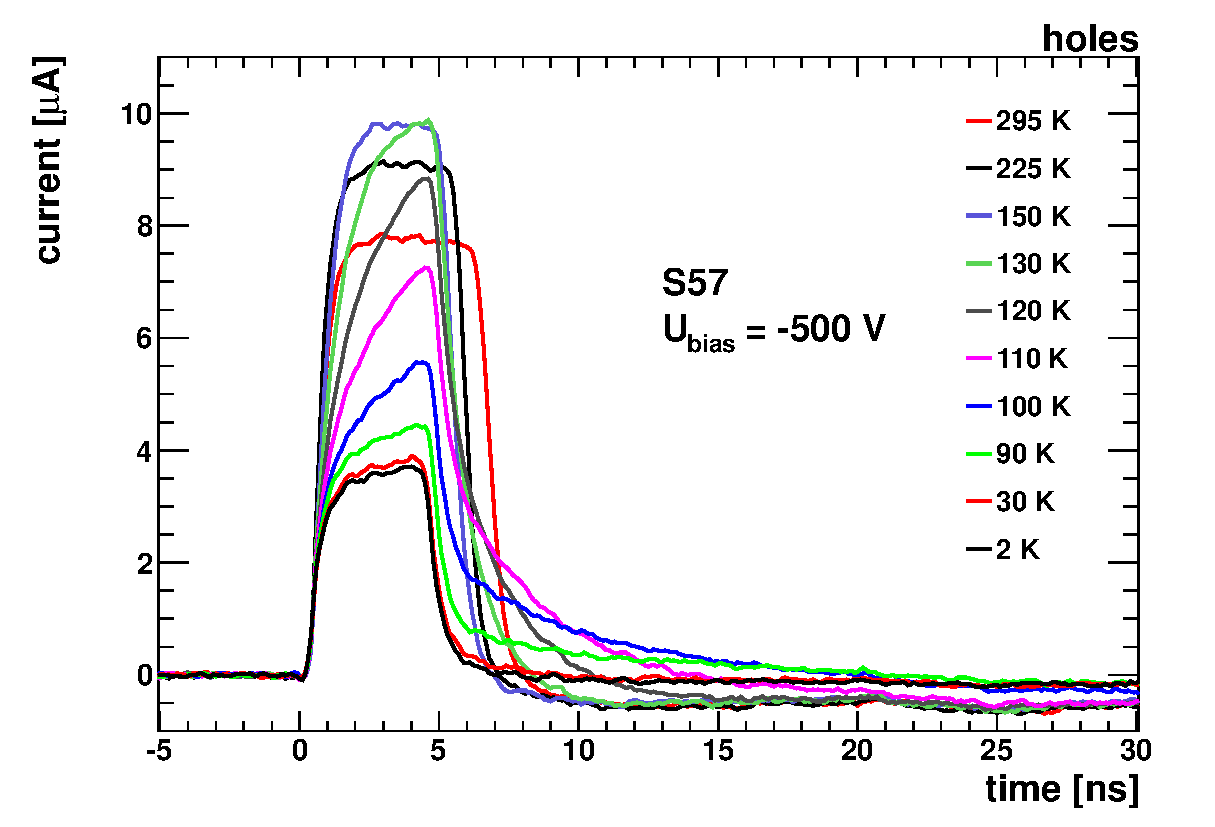
\includegraphics[width=0.49\textwidth]{figures/TCTholes500_exS57.eps}
 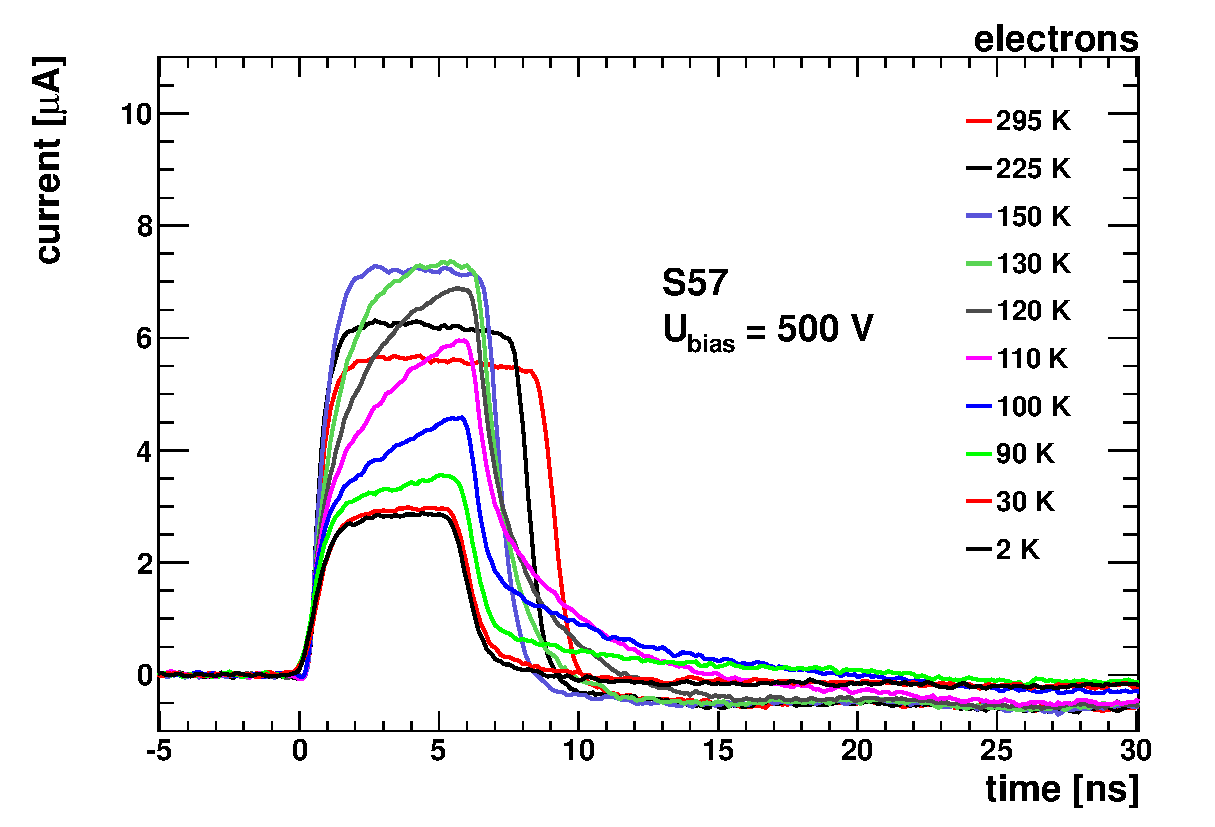
\includegraphics[width=0.49\textwidth]{figures/TCTelecs500_exS57.eps}
 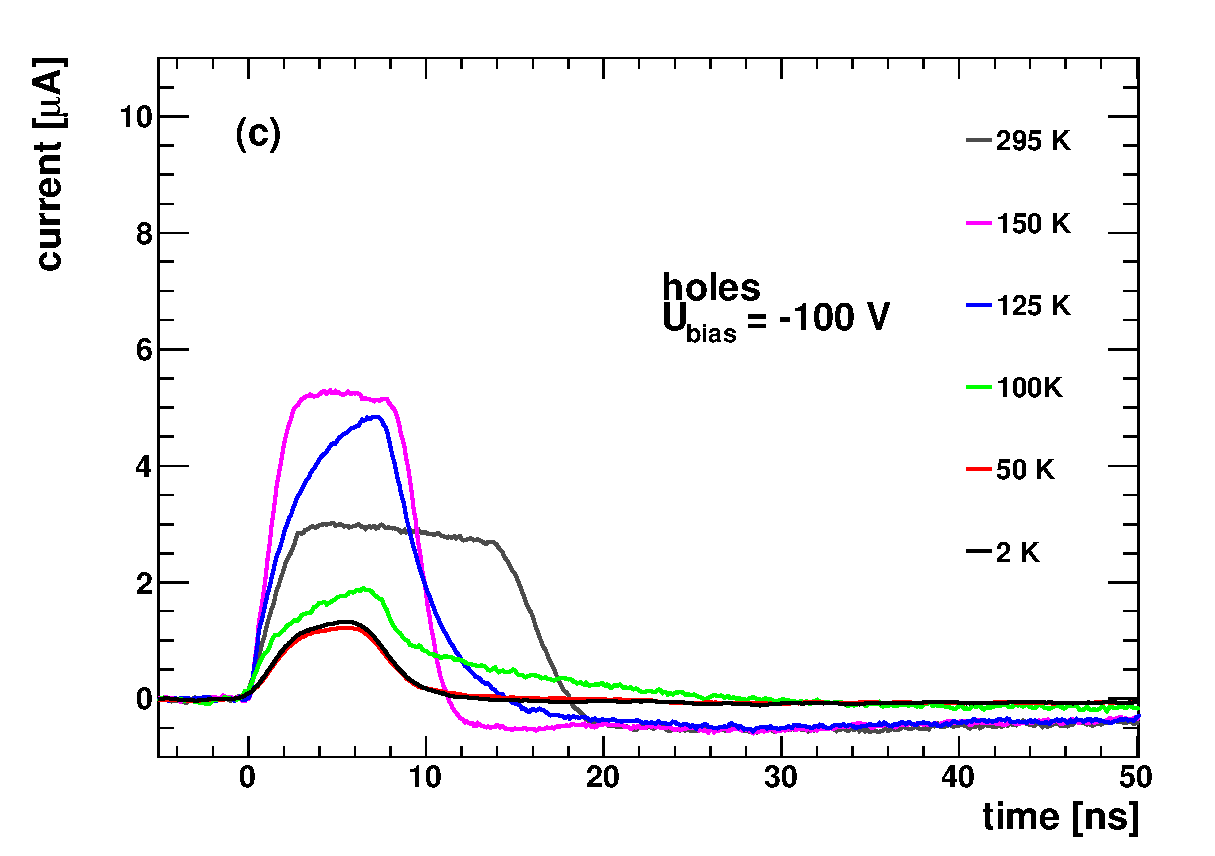
\includegraphics[width=0.49\textwidth]{figures/TCTholes100.eps}
 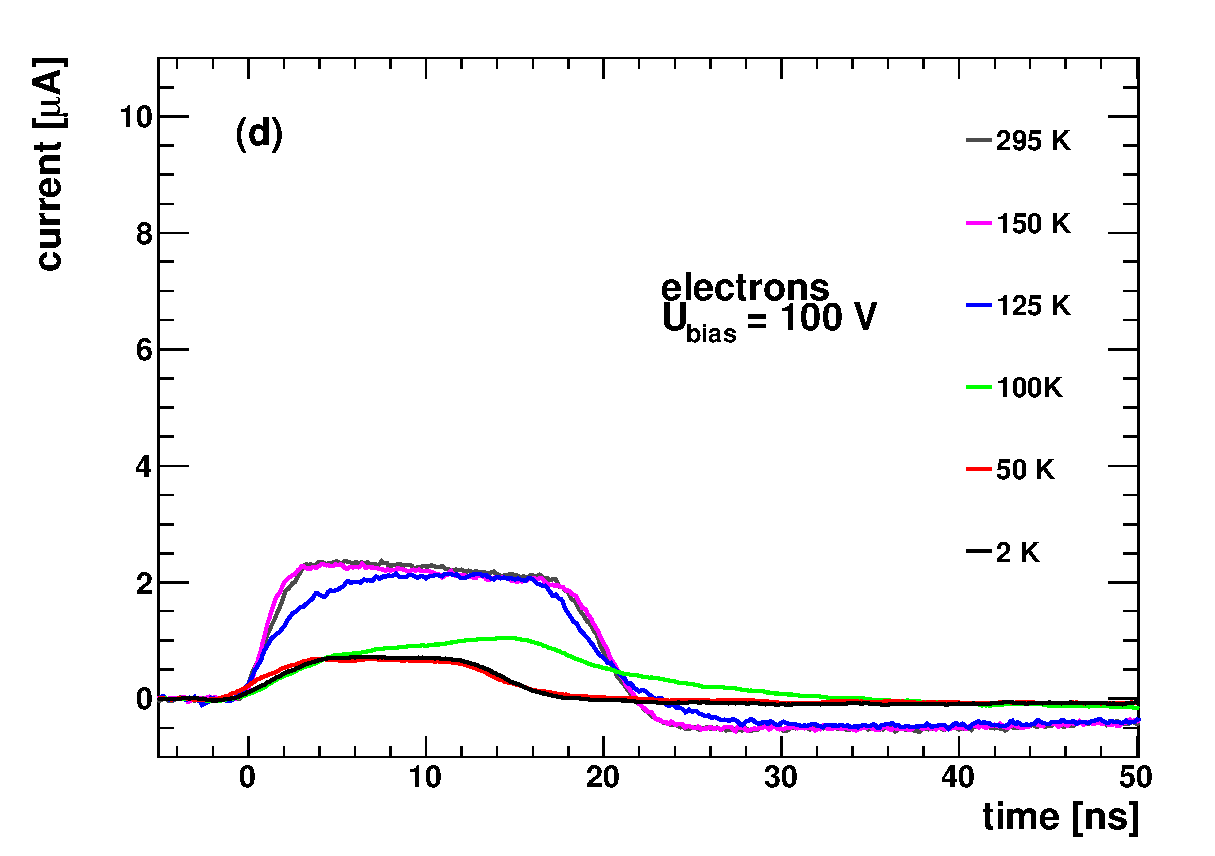
\includegraphics[width=0.49\textwidth]{figures/TCTelecs100.eps}

 \caption{Averaged current pulses for holes \textbf{(left column)} and electrons \textbf{(right column)} at various temperatures for
 $U_{\textrm{bias}} = \pm\SI{500}{\volt}$ \textbf{(top row)} and $U_{\textrm{bias}} = \pm\SI{100}{\volt}$ \textbf{(bottom row)} are shown for \textit{S57}.
 Note the similarity of electron pulses at $\SI{150}{\kelvin}$ and $\SI{295}{\kelvin}$. 
 Pulses from \textit{S52} and \textit{S79} are very similar and hence omitted.}
 \label{fig:currentprofiles}
\end{figure}

Hole and electron induced currents were recorded for temperatures between $T$ = 295\,K and  $\SI{2}{\kelvin}$. 
The set bias voltages covered a range from $ \SI{30}{\volt} \leq |V_{\textrm{bias}}| \leq \SI{900}{\volt}$ corresponding to electric field strengths from $\SI{0.06}{\volt/\um}$ to $\SI{1.8}{\volt/\um}$. 
Figure~\ref{fig:currentprofiles} shows a selection of the recorded and averaged pulses for SUT \textit{S57} at $\SI{\pm 500}{\volt}$ (top row) and $\SI{\pm 100}{\volt}$ (bottom row) for holes (left column)
 and electrons (right column). 
The electrons pulses are shown with an inverted current sign. 
Additional current pulses for samples \textit{S52} and \textit{S79} are published in \cite{JansenThesis}. 
At $\SI{\pm 500}{\volt}$, fast rise-times ($t_{\textrm{rise}} < \SI{1}{\nano\second}$) to about $\SI{2}{\micro\ampere}$  are observed for both hole and electron pulses for all temperatures. 
The time resolution for a single pulse (not averaged) at RT and $E = \SI{0.94}{\volt/\micro\meter}$ is $\sigma_{\textrm{t}} = \frac{\sigma_{\textrm{noise}}}{\textrm{slope}}
\leq \frac{\SI{0.4}{\micro\ampere}}{\nicefrac{\SI{7.2}{\micro\ampere}}{\SI{1}{\nano\second}}} = \SI{56}{\pico\second}$. 
At lower fields both the rise-time and the fall-time increase.

The rising edge of the signal marks the start of the charge drift. 
The falling edge marks the collection of charges at the opposite electrode. 
At RT the signal has an almost flat top during the drift as a consequence of the field being constant across our diamond samples. 
A net space-charge of the order of $\sim \SI{e11}{\e/\centi\meter^3}$ already leads to a significant change in pulse shape,
 i.e.~an exponential current behaviour~\cite{pernegger:073704}. 
Such intrinsic net space-charge seems to be absent in all three samples. 
For $\SI{\pm500}{\volt}$ ($E = \SI{0.94}{\volt/\micro\meter}$) the pulses become shorter with decreasing temperature
 due to higher carrier mobility as acoustic phonon scattering decreases with decreasing temperature.

The observed pulse shape depends strongly on the temperature between $\SI{75}{\kelvin}$ and $\SI{150}{\kelvin}$. 
The rising edge develops an $1-\exp \left(-t/\tau(T)\right)$ behaviour while the falling edge develops an equivalently long exponentially falling tail. 
Note that neither polarisation nor a non-zero net-effective space charge can explain the apparent temperature dependence of the shapes. 
The same effect on the pulse shape has been verified in all three SUTs.
A theoretical model explaining the temperature and electric field dependence of the pulse shape is laid down in the discussion section.
Here, we note that the signal can be decomposed into two parts: an almost rectangular one and a second comprising exponentially rising and falling flanks. 
The exponentially falling flank is a direct consequence of the exponentially rising flank. 

The drifting charges are collected at the opposing electrode after an average transit time $\ttr= \nicefrac{d}{\vdrift}$. 
This `release-drift-collect' scheme is depicted in Fig.~\ref{fig:collection} for two different start time distributions assuming a local charge deposition close to the incident electrode. 
If a function $\dot{N}_{\textrm{start}}(t)$ represents the distribution of the start time of the drift,
 the total number of charges that started to drift is $N_{\textrm{start}}(t) = \int_0^t \dot{N}_{\textrm{start}}(t)\,\dd t$. 
With the average transit time $\ttr = t_{\textrm{end}} - t_{\textrm{start}}$
 the distribution of the collection time of charges is $\dot{N}_{\textrm{end}}(t) = \dot{N}_{\textrm{start}}(t-\ttr)$, 
 and the total number of collected charges is $N_{\textrm{end}}(t) = \int_0^t \dot{N}_{\textrm{start}}(t-\ttr)\,\dd t$. 
The number of drifting charges is hence simply

\begin{equation}
 N_{\textrm{\drift}}(t) = N_{\textrm{start}}(t) - N_{\textrm{end}}(t) = N_{\textrm{start}}(t) - N_{\textrm{start}}(t-\ttr).  
 \label{eq:collection}
\end{equation}

\noindent
Figure~\ref{fig:collection} (A) depicts a Gaussian start time distribution resulting in an error-function-shaped, almost rectangular current pulse.
Correspondingly, an exponential start time distribution results in exponentially rising and falling flanks of the current pulses. 
We will argue in section~\ref{sec:discussion}, that the error-function-shaped part originates from charges in an \textit{outer region} and the exponential part from an \textit{inner region}.

\begin{figure}[tbp]
 \centering
 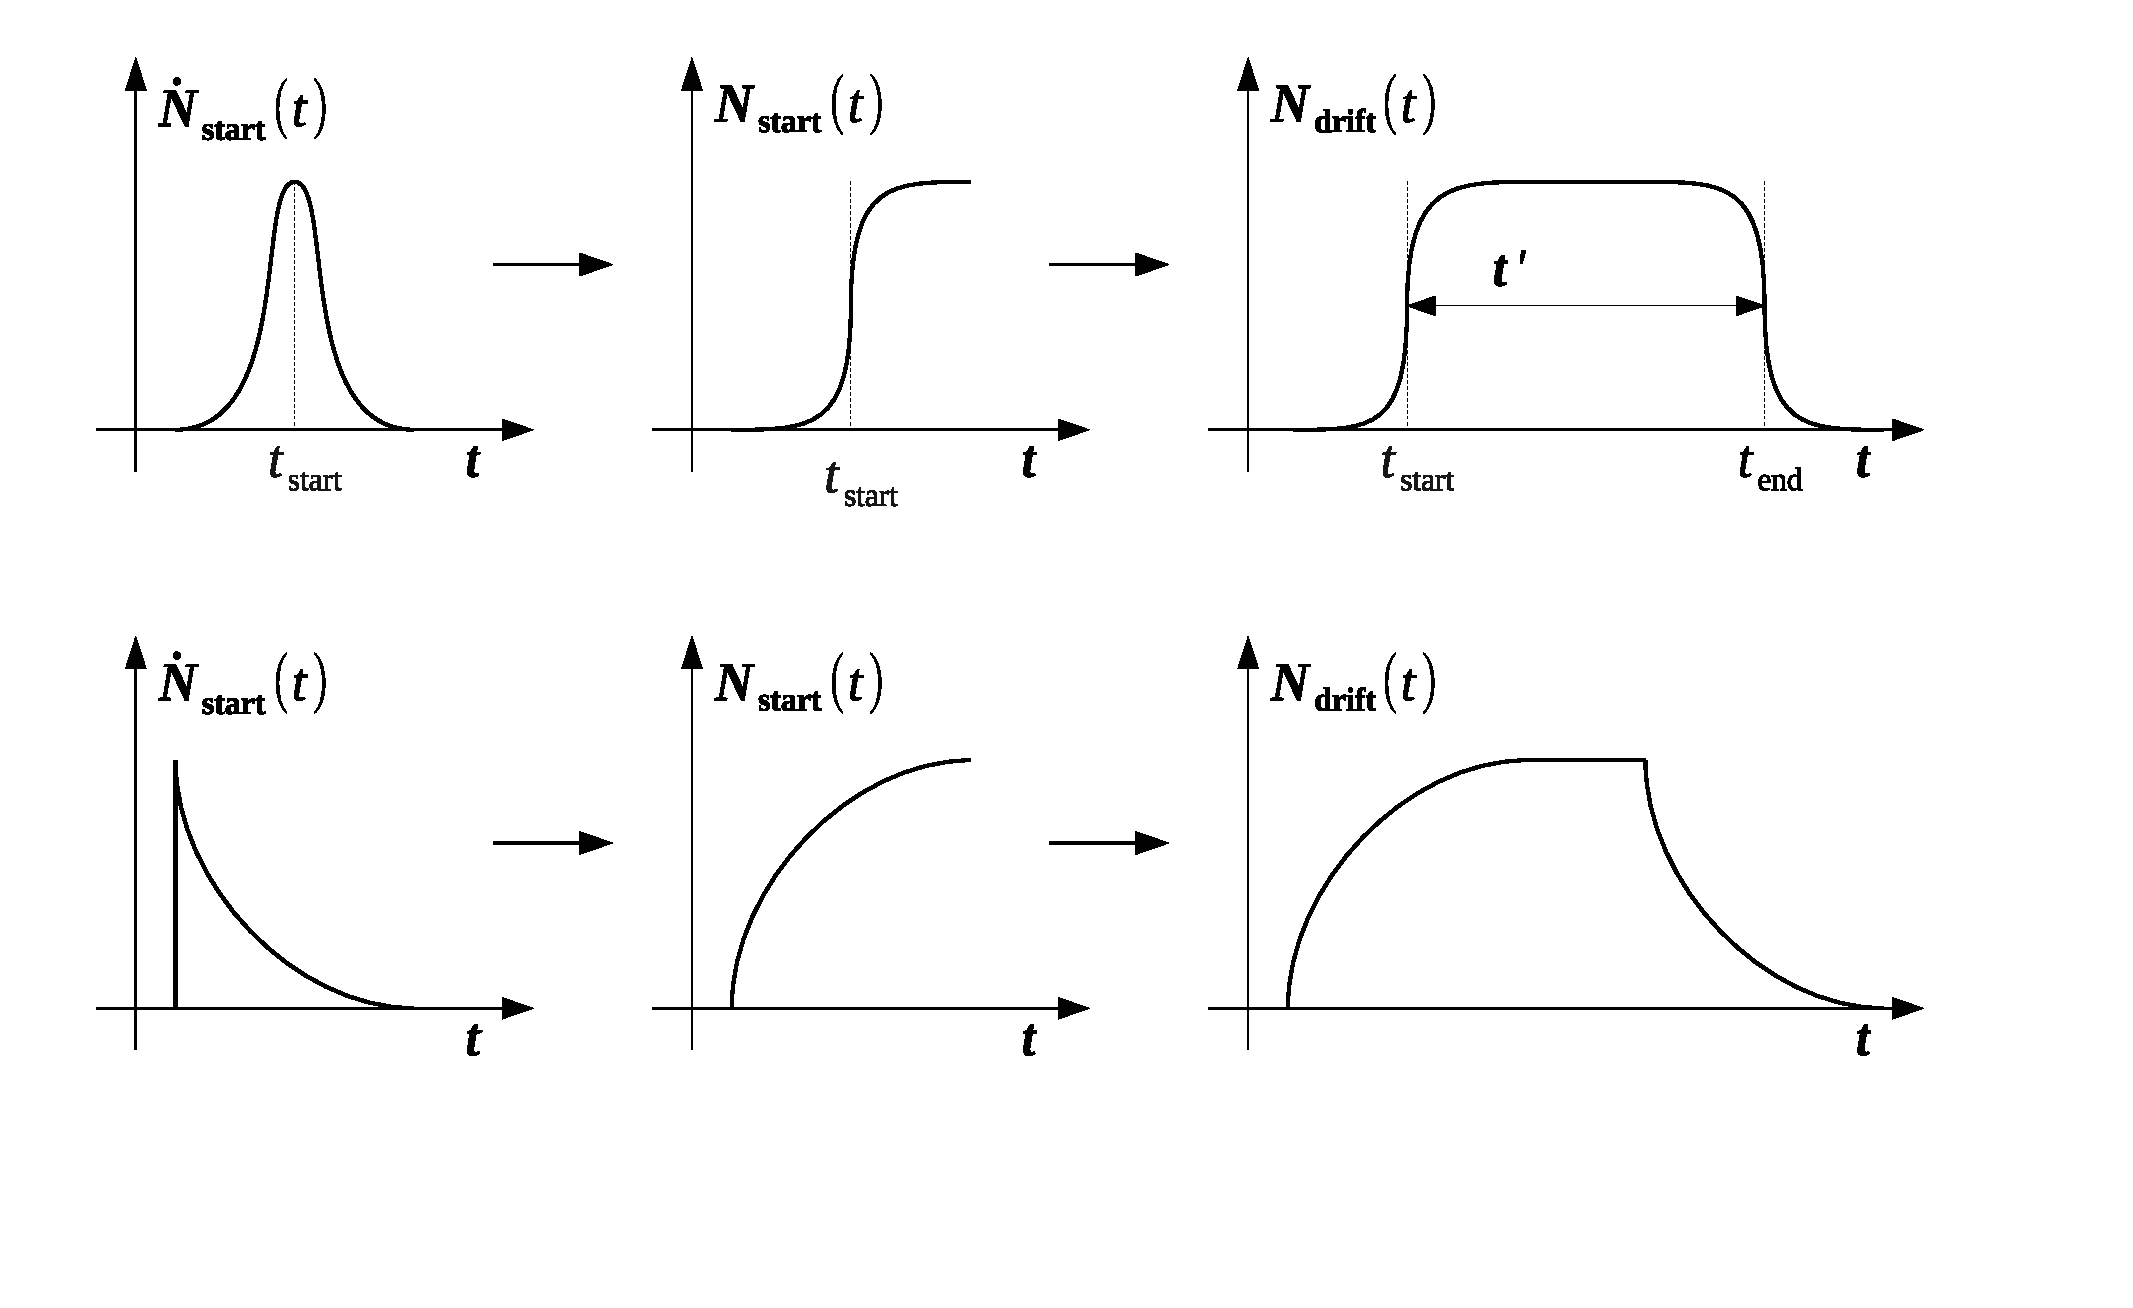
\includegraphics[trim=0cm 3cm 3.5cm 0cm, clip=true,width=0.79\textwidth]{figures/driftingcharges2.eps}
\put(-380,175){(A)}
\put(-380,69){(B)}
 \caption{\textbf{(A)} A Gaussian and \textbf{(B)} an exponential start time distribution function \textbf{(left column)},
 their resulting number of started charges distribution function \textbf{(middle column)}
 and the drifting charges distribution \textbf{(right column)} are shown.}
 \label{fig:collection}
\end{figure}


\subsection{Total integrated current}

\begin{figure}[tb]
 \centering
 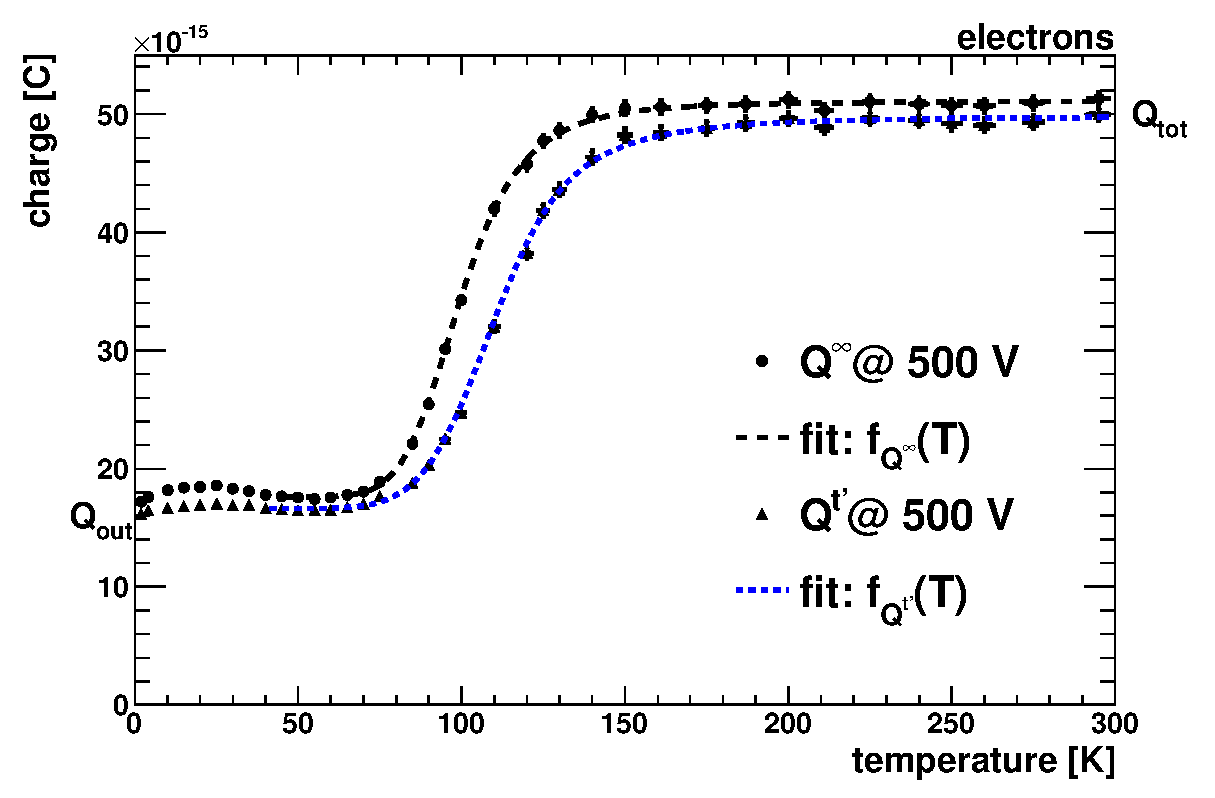
\includegraphics[width=0.49\textwidth]{figures/QttrTmultiE_e.eps}\put(-180,110){\LARGE (A)}\vspace{0.3cm}
 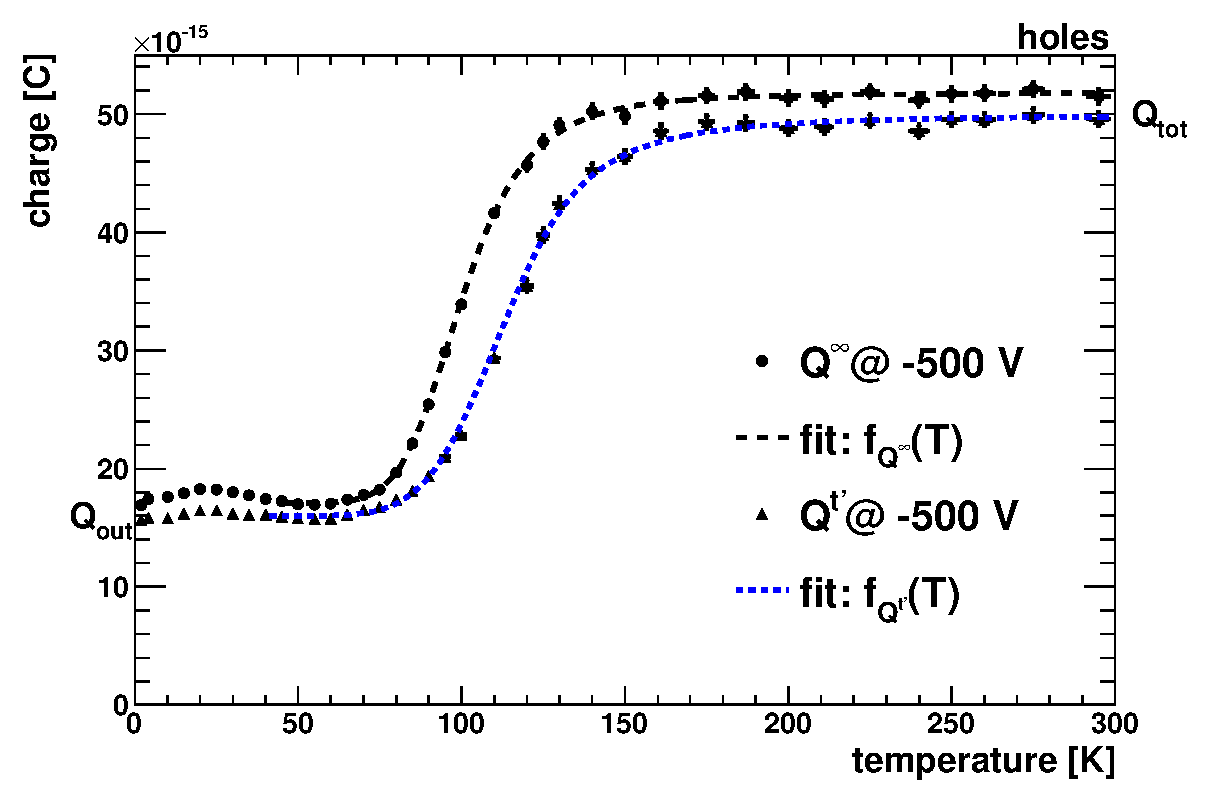
\includegraphics[width=0.49\textwidth]{figures/QttrTmultiE_h.eps}\put(-180,110){\LARGE (B)}
 \caption{The measured charge as a function of the temperature is shown for $Q^{\textrm{|infty}}$ and $Q^{t'}$ for \textbf{(A)} electrons and \textbf{(B)} holes.}
 \label{fig:QT}
\end{figure}

The measured current is integrated over time and analysed as a function of temperature, which is shown in 
 Fig.~\ref{fig:QT} for electrons \textbf{(A)} and holes \textbf{(B)} at $E \approx \SI{1}{\volt/\micro\meter}$, or an applied voltage of $\SI{500}{\volt}$. 
An S-curve describes the overall shape of the measured charge. 
Two variations of the collected charge are shown, the upper one, $Q^{\infty}$, integrates the current including the exponentially falling tail,
 the lower one, $Q^{t'}$ integrates up to the transit time omitting the tails. 
The statistical uncertainty on the charge is estimated to be around 1\,\%. 
The integral of the current pulses is constant at about $Q = \SI{52.0(5)}{\femto\coulomb}$ between room temperature and $\SI{150}{\kelvin}$,
 decreases to about one third of the RT value towards $\sim$ $\SI{75}{\kelvin}$, and remains at this level towards even lower temperatures.
The fit-function, justified in section~\ref{sec:discussion}, contains four parameters: (1) the total charge, (2) the \textit{outer} charge, cf.\ section~4, and (3) a factor $\varepsilon$ in combination with a
 Boltzmann factor 
 with (4) an activation energy $\Ea$. 
The total charge $\Qtot$ and the outer charge $\Qo$ are highly predetermined by the two plateaus before and after the charge drop at about 52\,fC and 17\,fC, respectively, 
 and the inner charge is then $\Qin = \Qtot - \Qo$. 
The fit function for the measured charge $Q^{\infty}$ becomes

\begin{equation}
 f_{Q^{\infty}}(T) = \Qo + \frac{\Qin}{1+\varepsilon\cdot\exppEa},\phantom{\frac{\tau}{\ttr}\exp{\left(-\ttr/\tau\right)}}.
 \label{eq:fitQinfty}
\end{equation}

The fit-function for $Q^{t'}$ is more complicated, as it involves the transit time $\ttr$ and the shape constant $\tau$. 
Therefore, it contains five free parameters ($\Qtot$, $\Qo$, $\varepsilon$, $\Ea$, $\tau$). %, again with $\Qtot$ and $\Qo$ highly predetermined. 
$\ttr$ is taken from data, cf. section~\ref{sec:tt},
 i.e.~a simple power law fit of the transit time as a function of the temperature at $E \approx \SI{1}{\volt/\micro\meter}$. 
The fit-function then reads

\begin{equation}
 f_{Q^{t'}}(T) = \Qo + \frac{\Qin}{1+\varepsilon\cdot\exppEa}\cdot \frac{\tau}{\ttr} \cdot \left[ 1 - \frac{\tau}{\ttr} (1 - \exp{\left(-\ttr/\tau\right)}  ) \right] ,
 \label{eq:fitQtprime}
\end{equation}

\noindent
with a shape constant $\tau$ describing the exponential flanks. 

\begin{table}[tb]
 \centering
 \caption{The results of fitting, firstly, Eq.~(\ref{eq:fitQtprime}) to the charge collected until $\ttr$ ($Q^{t'}$, i.e.~without the tail)
 and secondly Eq.~(\ref{eq:fitQinfty}) to the charge including the tail ($Q^{\infty}$) are listed for electrons and holes at a bias voltage of 500\,V. {\color{red}(A3)}}
   \vspace{0.5cm}

 \begin{tabular}{lcccccc}
\toprule
 & \multicolumn{6}{c}{$Q^{t'}$}  \\  \midrule% \cmidrule(r){2-6} \cmidrule(l){7-10}
 & $\Qtot$\,[fC] & $\Qo$\,[fC] & $t_{e,0}$\,[ps] &  $\taurec$\,[ns]  & $\Ea$\,[meV]& $\chi^2/\textrm{ndf}$\\
% &  fixed	 &  free       & free  &  free     &                             & fixed         & free        & free                           & \\
\midrule
 $\e$ & $\num{49.8(2)}$ & $\num{16.6(3)}$ & $\num{0.6(2)}$ & $\num{14}$ (fixed) & $\num{79(3)}$ & 0.9 \\
 $\h$ & $\num{50.0(2)}$ & $\num{16.0(3)}$ & $\num{1.1(3)}$ & $\num{14}$ (fixed) & $\num{76(3)}$ & 1.4 \\ \midrule
 & \multicolumn{6}{c}{$Q^{\infty}$}\\ \midrule
 & $\Qtot$\,[fC]   & $\Qo$\,[fC]     &  $\num{e5}\,\varepsilon$  & & $\Ea$\,[meV] & $\chi^2/\textrm{ndf}$ \\ 
 \midrule
$\e$ & $\num{51.1(2)}$ & $\num{17.6(3)}$ & $\num{2.8(9)}$     & & $\num{90(3)}$ & 0.4\\
$\h$ & $\num{51.8(2)}$ & $\num{17.1(3)}$ & $\num{5.1(15)}$    & & $\num{85(3)}$ & 0.5\\
avg  & 51.5            & 17.4            & $\num{3.4(8)}$     & & $\num{87.5(22)}$ & \\
\bottomrule
 \end{tabular}
 \label{tab:fitQ}
\end{table} %FIXME re-fit, paste values

{\color{red}(A2)} [The result of the fits for $Q^{t'}$ and $Q^{\infty}$ are tabulated in Tab.~\ref{tab:fitQ} for both carrier types
 and the fit-functions are superimposed as dotted lines in Fig~\ref{fig:QT}. 
The inner charge constitutes about 2/3 of the total charge at a field of $E = \SI{1}{\volt/\micro\meter}$, the outer charge about 1/3,
 summing to a total of about 52\,fC. 
Estimates of $t_{e,0}$ and $\taurec$ are obtained by the following consideration. 
At around 100\,K, $\Qin$ has decreased to half of its RT value, see Fig.~\ref{fig:QT}. 
Therefore $\frac{1}{1+\frac{\tauevap}{\taurec}} = \frac{1}{2}$ and hence $\tauevap = \taurec$. 
With a measured shape constant of $\SI{7}{\ns}$ at 100\,K, cf.\ section~3.5, both the recombination lifetime and the evaporation time at 100\,K are $\sim$ $\SI{14(2)}{\ns}$,
 and therefore $\tauevap = t_{e,0} \exppEa \approx \SI{14}{\ns}$.
Thus, $t_{e,0}$ becomes 

\begin{equation}
 t_{e,0} = \SI{14(2)}{\ns} / \exp{\big( \SI{0.0875}{\eV}/(\kB\cdot \SI{100}{\kelvin}) \big)} = \SI{0.5(1)}{\ps}.
\end{equation}

\noindent
(!) The fit $f_{Q^{t'}}$ does not converge for $\taurec$, we therefore fixed $\taurec$ at a reasonable value of $\taurec = \SI{14}{\ns}$. 
Then, the fit yields
\begin{equation}
 t_{e,0} = \SI{0.6(2)}{ps}
\end{equation}
 
\noindent
in reasonable accordance with the earlier evaluated $t_{e,0}$-value.  
A third estimation results from the $Q^{\infty}$-fit (Eq.~(\ref{eq:fitQinfty})), where only the ratio $\varepsilon = t_{e,0}/\taurec$ appears:
\begin{equation}
 \varepsilon = t_0/\taurec = (\num{3.4(8)})\,\num{e-5}
\end{equation} 

\noindent
averaging the results from electrons and holes, see Tab.~\ref{tab:fitQ}. 
Using again the evaporation time $\tauevap \approx \SI{14(2)}{\ns}$, it is found that

\begin{equation}
 t_{e,0} = \SI{14(2)}{\ns} \cdot \varepsilon = \SI{0.5(2)}{\ps}.
\end{equation}

\noindent
With $t_{e,0} \approx \SI{0.5}{\ps}$, the evaporation time at 50\,K, 150\,K and 300\,K follow to be of the order of $\SI{600}{\micro\second}$, $\SI{600}{\micro\second}$ and $\SI{30}{\ps}$, respectively. 
It is emphasised that the experimentally found scale of $t_{e,0}$ is crucial for the description of the observed data.
If $t_{e,0}$ was of the order of femtoseconds, the charge would not have decreased to half of its RT value at 100\,K, but at 58\,K. 
Also, the rise time of the current pulse at 150\,K would have increased to ??, which is experimentally not observed. 
In the same manner, activation energies of the order of 40\,meV are strictly excluded. 
]

\begin{figure}[tb]
 \centering
 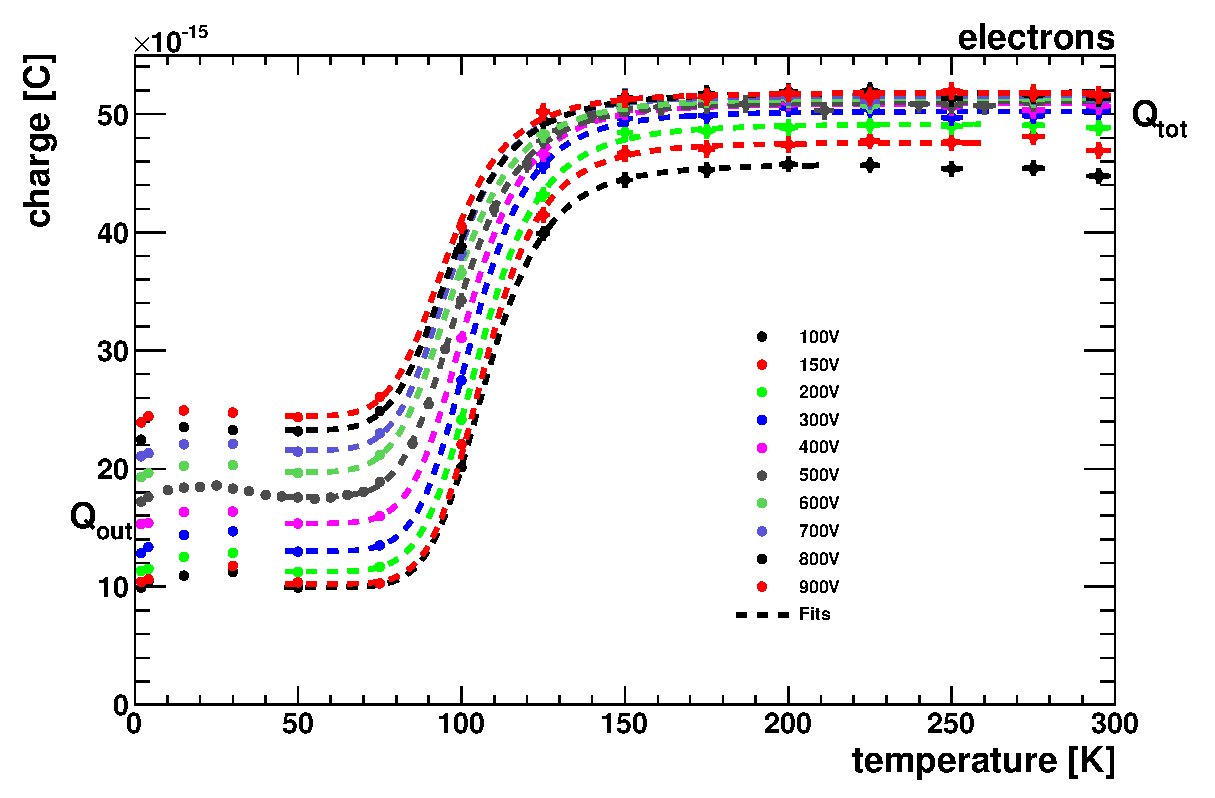
\includegraphics[width=0.49\textwidth]{figures/QTmultiE_e.eps}\put(-180,120){(A)}\vspace{0.3cm}
 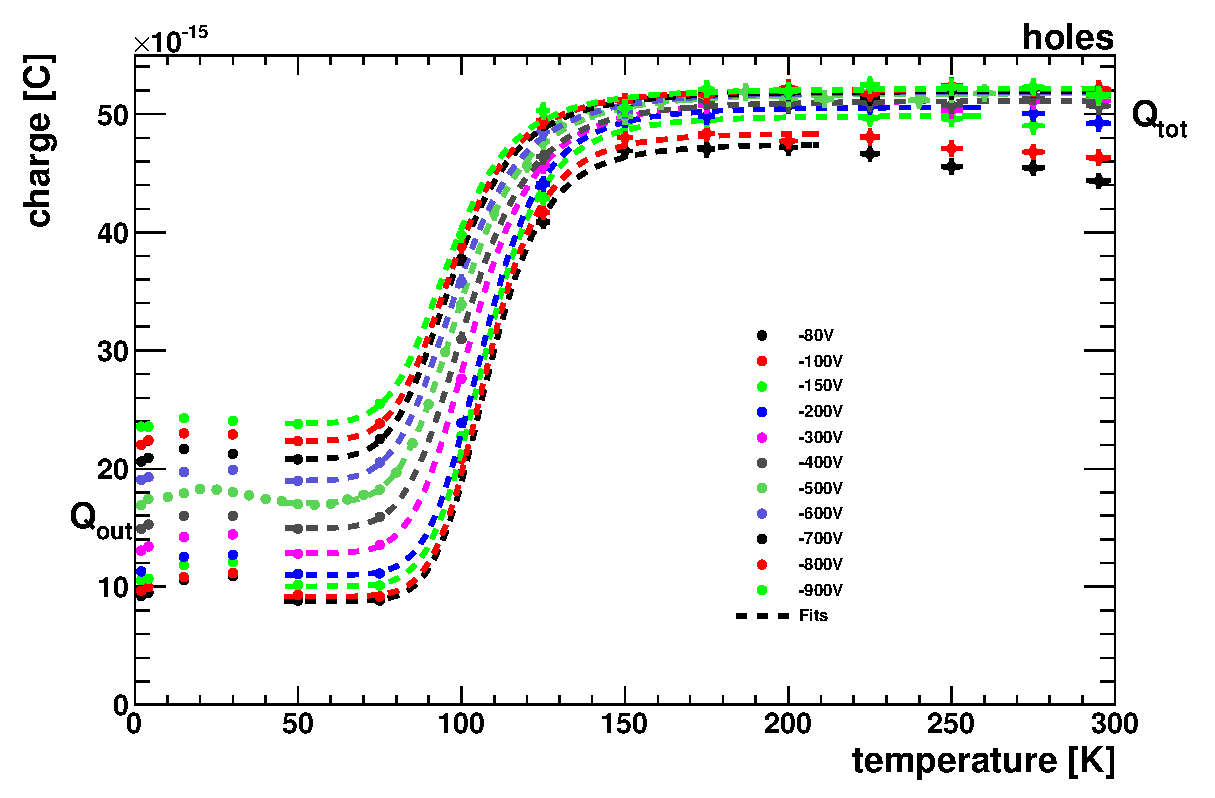
\includegraphics[width=0.49\textwidth]{figures/QTmultiE_h.eps}\put(-180,120){(B)}
 \caption{The measured charge $Q^{\infty}$ as a function of the temperature is shown for various voltages for electrons \textbf{(A)} and holes \textbf{(B)}.}
 \label{fig:QTvoltage}
\end{figure}

The S-curves for different voltages are shown for $Q^{\infty}$ in Fig.~\ref{fig:QTvoltage}. 
Again, the similarity between electron and hole pulses is evident. 
The fit described earlier is performed for charge data from 100\,V to 900\,V, each fit resulting in a value for $\varepsilon$, and $\Ea$. 
The discussion of the temperature dependence of the fit-parameters ist postponed to section~\ref{sec:discussion}. 

\begin{figure}[tb]
 \centering
 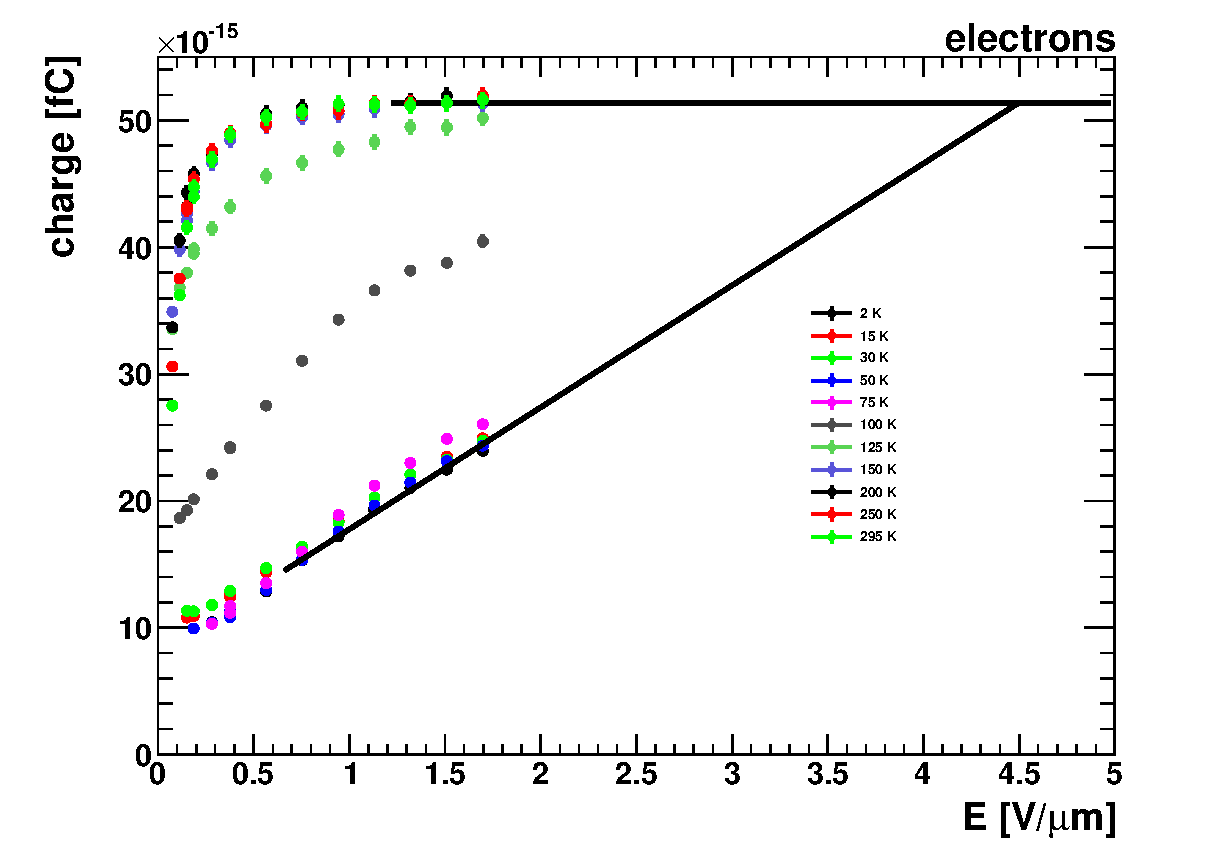
\includegraphics[width=0.49\textwidth]{figures/QEmulti_e}\put(-180,120){(A)}\vspace{0.3cm}
 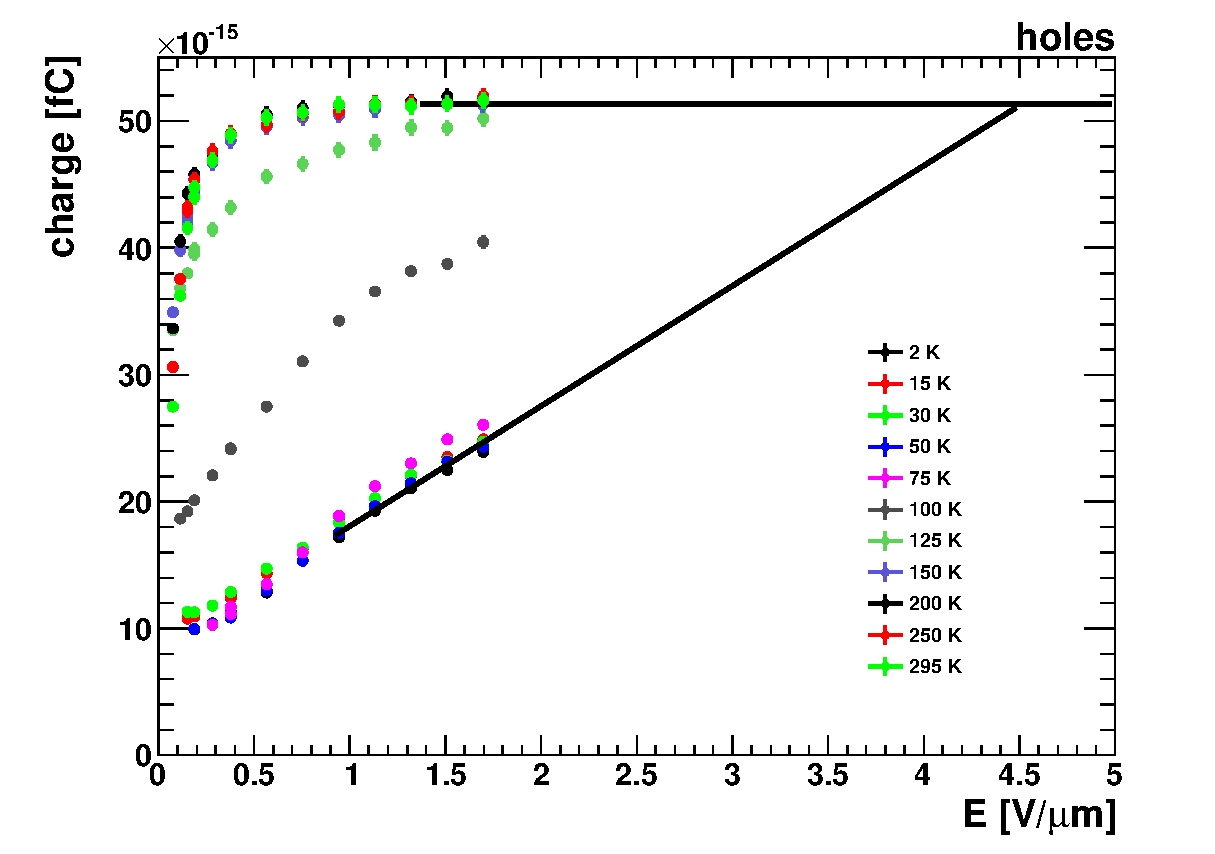
\includegraphics[width=0.49\textwidth]{figures/QEmulti_h}\put(-180,120){(B)}
 \caption{The measured charge $Q^{\infty}$ as a function of the applied field strength is shown for various temperatures for electrons \textbf{(A)} and holes \textbf{(B)}.}
 \label{fig:QvsE}
\end{figure}

Plotted as a function of the electric field strength, the influence of the field on the measured charge becomes evident.
Figure~\ref{fig:QvsE} shows the same behaviour for all temperatures above 150\,K, and below 75\,K. 
The first increases rapidly with field strength and reaches a flat top at about $\SI{1}{\volt/\micro\meter}$, whereas the latter increases linearly. 
The discussion of this behaviour is covered in section~4. 

\subsection{Fit-function for the current pulses}

The transit time and characteristic time constant are determined by the time difference between end time and start time of drift,
 $t_{\text{e}}$ and $t_{\text{s}}$ respectively, hence $\ttr = t_{\text{e}} - t_{\text{s}}$.
A function $f(t;P)$ is fitted to each current pulse in order to find $t_{\text{e}}$ and $t_{\text{s}}$.
$f(t;P)$ is a function of time and a set of parameters $P$ incorporating two complementary error functions $(2-\Erfc(t-t_{\text{s}}))$ and $\Erfc(t-t_{\text{e}})$
 describing the rising and the falling edge, respectively. 
Additionally, an exponential component  of the form $\left( 1-\exp \left(-(t-t_{\text{s}})/\tau\right) \right) - \Theta_{\textrm{col}}(t;t_{\text{e}})$ with
  $\Theta_{\textrm{col}}(t;t_{\text{e}}) = 1 - \exp \left( -(t-t_{\text{e}})/\tau \right)$ for $t > t_{\text{e}}$ and $\Theta_{\textrm{col}}(t;t_{\text{e}}) = 0$ otherwise,
 is allowed, cf.~Eq.~(\ref{eq:collection}). 
The error functions describe a Gaussian probability distribution for the start time of the drift around $t_{\text{s}}$,
 and respectively a collection at the opposite electrode around $t_{\text{e}}$. 
The 50\% points mark $t_{\text{s}}$ and $t_{\text{e}}$, respectively. 
The fit parameter $\tau$ is given a physical meaning in the discussion section. 

At all temperatures and fields, the fit-function describes well the measured pulse shape of $i_m(t)$;
 each fit resulting in a value for $\tau(T,E)$ and $\ttrans(E,T)$.
One example of a fit to a measured pulse $i_m(t)$ at 100\,K and 500\,V is shown in Fig.~\ref{fig:ExModel2}. 
The resulting shape constant is $\tau(\SI{100}{\kelvin},\,\SI{500}{\volt}) \approx (\num{6.8}\pm\num{0.1}_{\textrm{stat}}\pm\num{1.0}_{\textrm{sys}})\,\si{\ns} \approx \SI{7(1)}{\ns}$. 
The current induced from charges stemming from the outer and the inner part of the cloud are shown separately as dashed lines
 featuring the error-function shape and the exponential shape, respectively.
The sum forms the solid line on top of the data. 
At this temperature, a certain fraction of the charge recombines. 

\subsection{Characteristic time constant}

\begin{figure}[t]
 \centering
 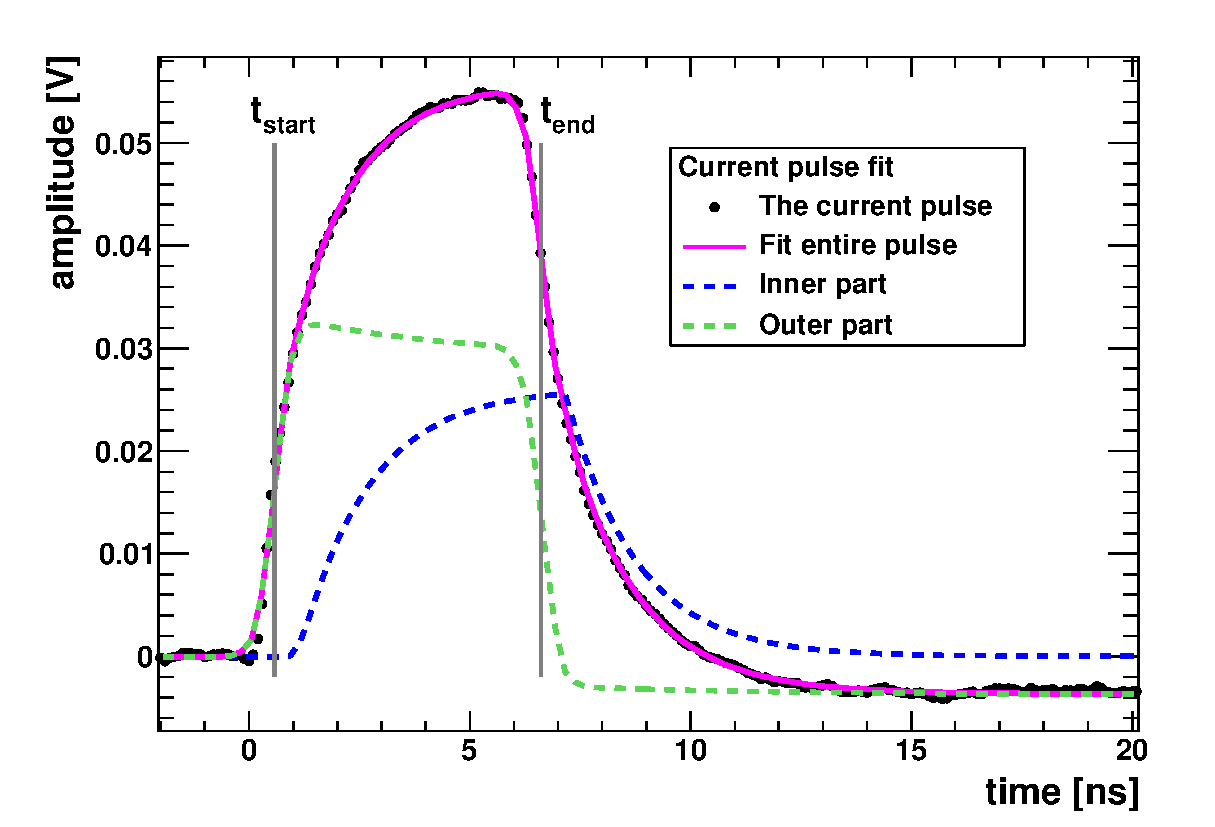
\includegraphics[width=0.59\textwidth]{figures/ex_pulsefit3}%pulseFit.C
 \caption{The fit to the measured pulse at 100\,K and 500\,V and its components are depicted.}
 \label{fig:ExModel2}
\end{figure}


The fitted shape constant $\tau$ is shown in Fig.~\ref{fig:fittau}
 as a function of temperature (closed circles) at $E \approx \SI{1}{\volt/\micro\meter}$. 
The error bars are the statistical errors resulting from the fit. 
For both electrons and holes $\tau$ remains about constant at $\SI{0.4}{\ns}$ between RT and $\SI{150}{\kelvin}$. 
Between $\SI{150}{\kelvin}$ and $\SI{90}{\kelvin}$, the shape constant increases steeply.%
\footnote{A comparison to measured values in the literature is difficult, or impossible,
 as no measurement of exciton properties in diamond using electric fields are known to the authors.}
Due to the decrease of the amplitude of the tail in the current pulses with decreasing temperature, the signal-to-noise ratio at $T \leq \SI{90}{\kelvin}$
 is too small in order to accurately fit the shape constant. 
The fitted $\tau$ therefore decreases for $T < \SI{90}{\kelvin}$. 
The corresponding region is marked as `insensitive'. 

\begin{figure}[t]
 \centering
  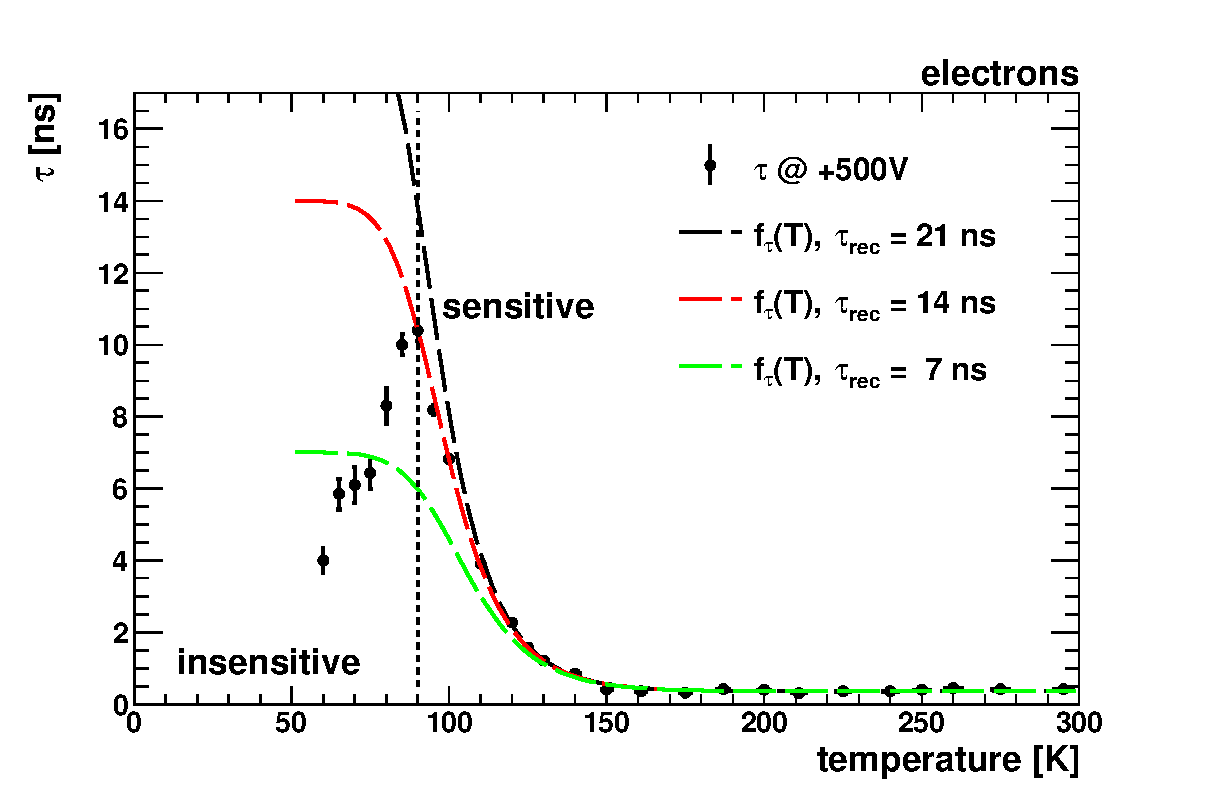
\includegraphics[width=0.49\textwidth]{figures/tauvsT_e}\put(-190,110){(A)}
  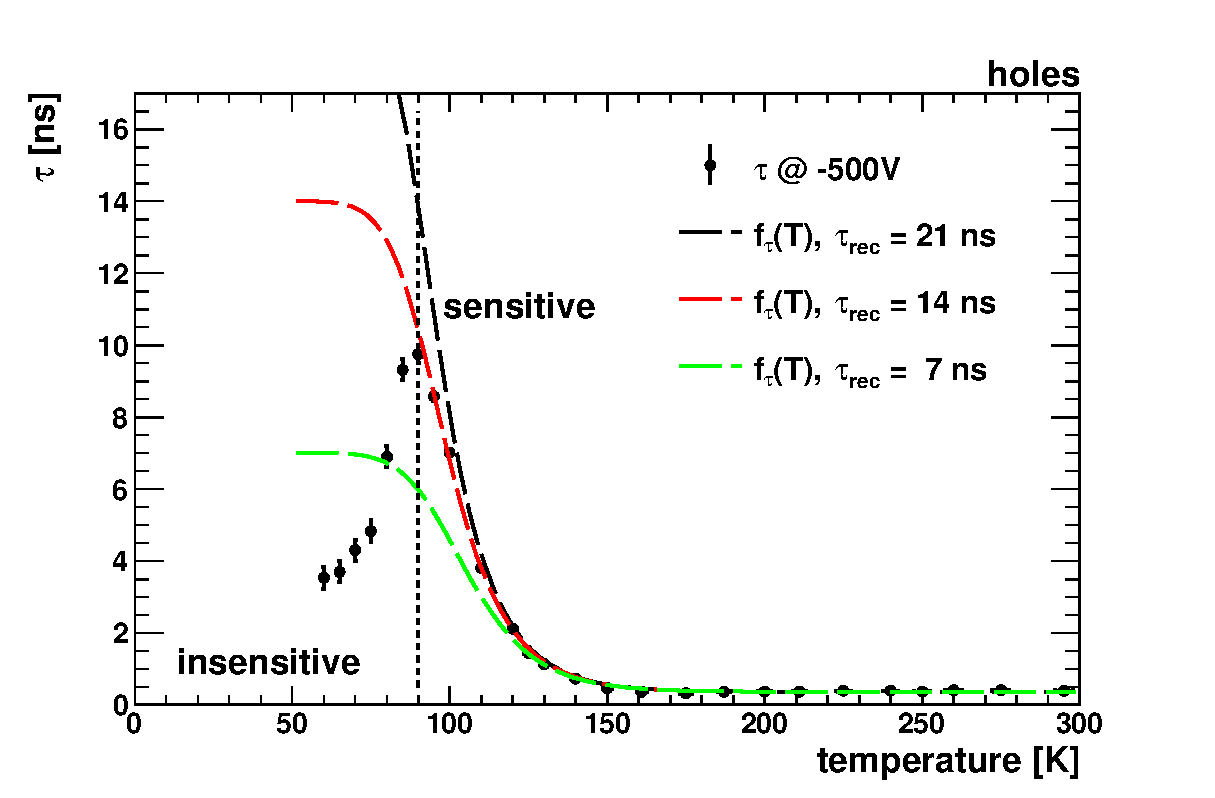
\includegraphics[width=0.49\textwidth]{figures/tauvsT_h}\put(-190,110){(B)}\\
  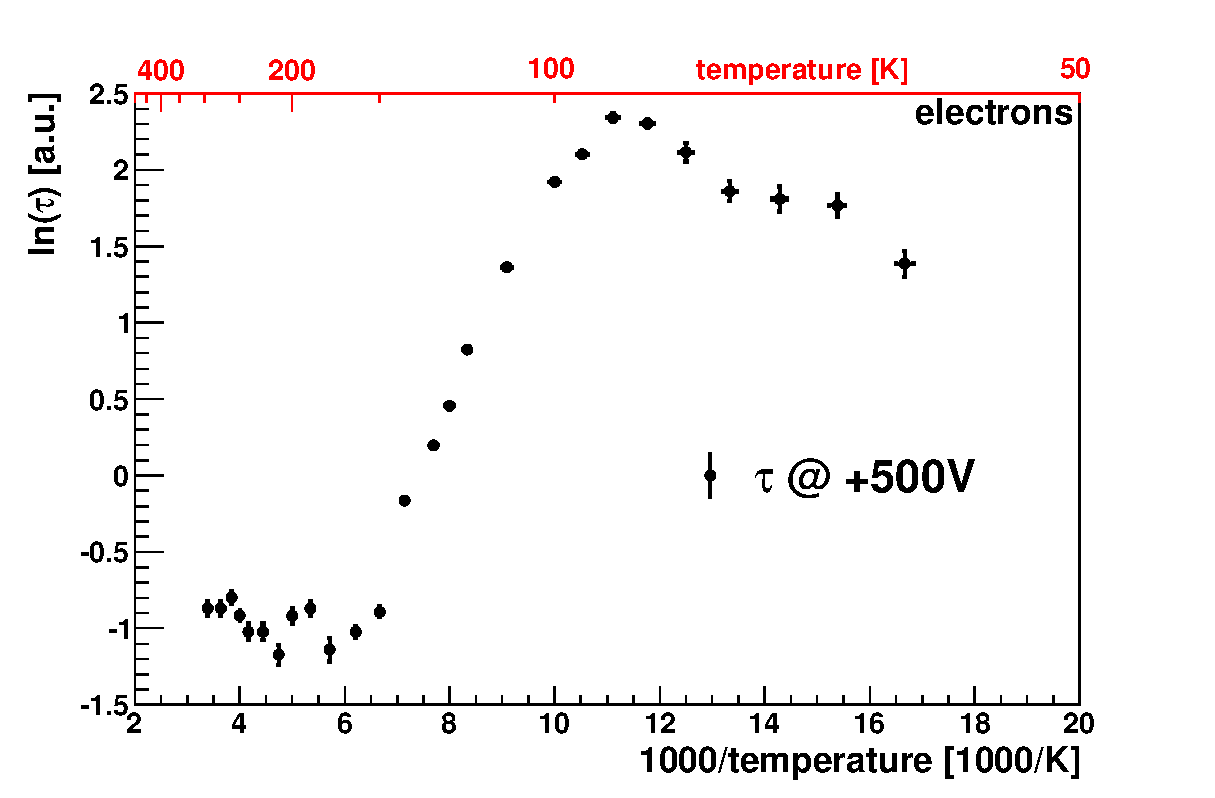
\includegraphics[width=0.49\textwidth]{figures/logtauvsTinv_e}\put(-190,110){(C)}
  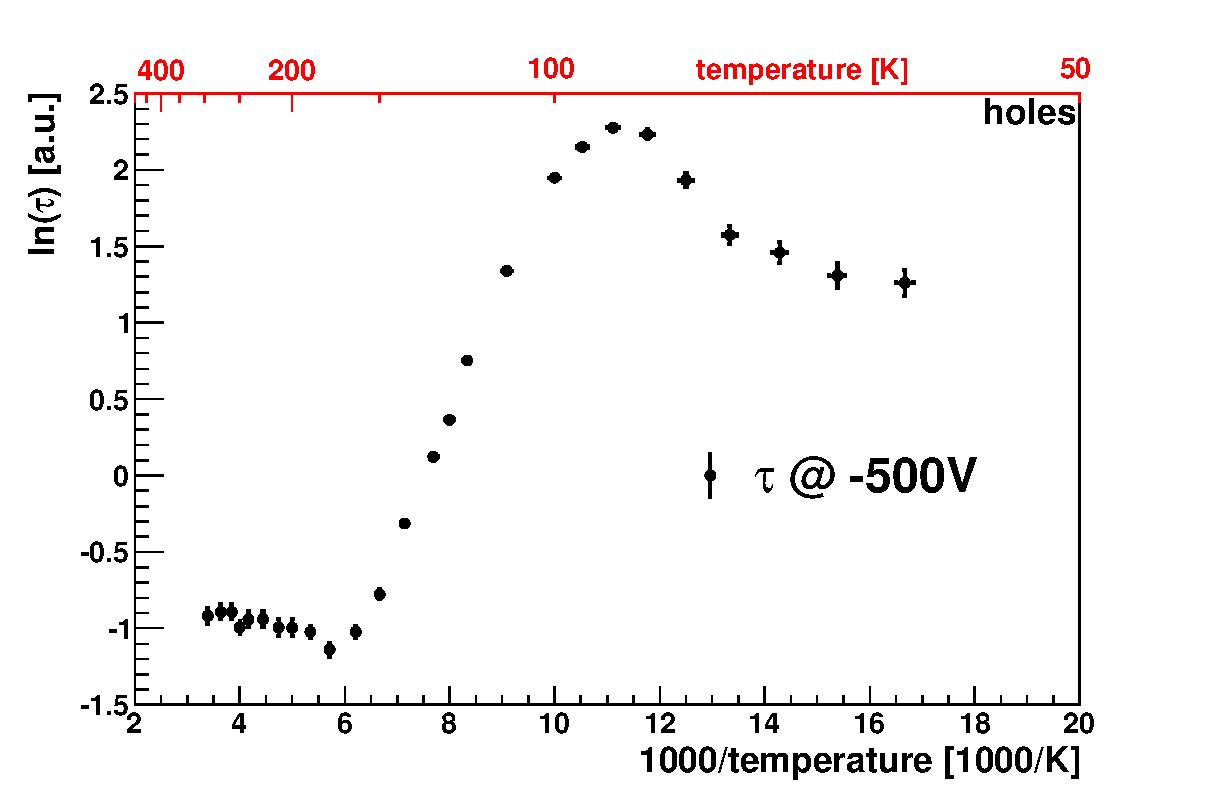
\includegraphics[width=0.49\textwidth]{figures/logtauvsTinv_h}\put(-190,110){(D)}
 \caption{The fitted shape constant $\tau$ is shown as a function of the temperature for electrons \textbf{(A)} and holes \textbf{(B)} at $500$\,V.
\textbf{(C)} and \textbf{(D)} show the results in $\ln{(\tau)}$ vs.~the inverse temperature.}
 \label{fig:fittau}
\end{figure} %FIXME title x-axis = 1000/temperature

We revise, if the measured temperature dependence of $\tau$ can be explained within the exciton model
 using the $t_{e,0}$-value (0.5\,ps) extracted from charge data. 
Using $\frac{1}{\tauzero} =  \frac{1}{\taurec} + \frac{1}{\tauevap}$ and $\tauevap = t_{e,0} \exppEx$ one finds

\begin{equation}
 \tauzero(T) = \left( \frac{1}{\taurec} + \frac{1}{\tauevap(T)} \right)^{-1} = \left( \frac{1}{\taurec} + \frac{1}{t_{e,0} \exppEx }\right)^{-1}.
 \label{eq:tauT}
\end{equation}

\noindent
A possible temperature dependence of the recombination lifetime is not allowed for. 
It is further important to notice that
 the fitted shape constant cannot be faster than the cut-off time constant, which arises from the cut-off frequency of the measuring system. 
In fact, the cut-off constant adds quadratically to the physical shape constant, resulting in the fitted shape constant.
Using Eq.~(\ref{eq:tauT}) and an additional such parameter $\tau_{cut}$, a function $f_{\tau}(T)$ is defined  as

\begin{equation}
 f_{\tau}(T) = \sqrt{\left( \frac{1}{\taurec} + \frac{1}{t_{e,0} \exppEx }\right)^{-2} + \left( \tau_{\textrm{cut}}\right)^2},
 \label{eq:fittau}
\end{equation}

\noindent
which is to be checked against the data. 
Superimposed in Fig.~\ref{fig:fittau} as dashed lines are $f_{\tau}(T)$ with the activation energy $\Ea = \SI{87.5}{\milli\eV}$, $t_{e,0} = \SI{0.5}{\ps}$,
 and three different $\taurec = 7,14,\SI{21}{\nano\second}$. 
It is clear from Fig.~\ref{fig:fittau} that Eq.~(\ref{eq:fittau}) describes the experimental data reasonably well
 using the afore mentioned $\Ea(\SI{500}{\volt}) = \SI{87.5}{\milli\eV}$, $t_{e,0} = \SI{0.5}{\ps}$, and $\taurec = \SI{14}{\ns}$. 
Therefore, a combination of values $\Ex$ and $t_{e,0}$ exists that consistently explains two important parts of the data,
 i.e.~the temperature dependence of both the measured charge and the fitted shape. 

The characteristic time constant shall also be studied as a function of the temperature in order to extract the activation energy as a function of the electric field. 

\begin{figure}[t]
 \centering
  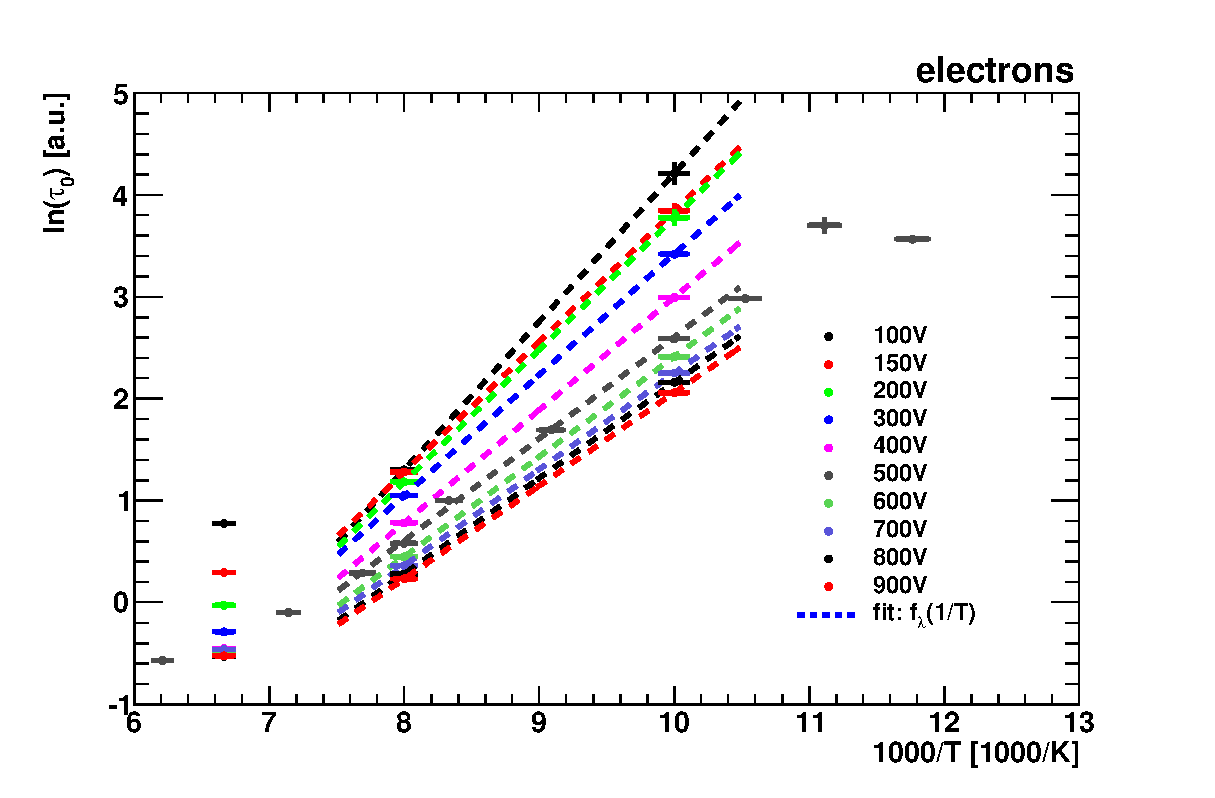
\includegraphics[width=0.49\textwidth]{figures/logtauvsTinvU_e}\put(-190,110){(A)}
  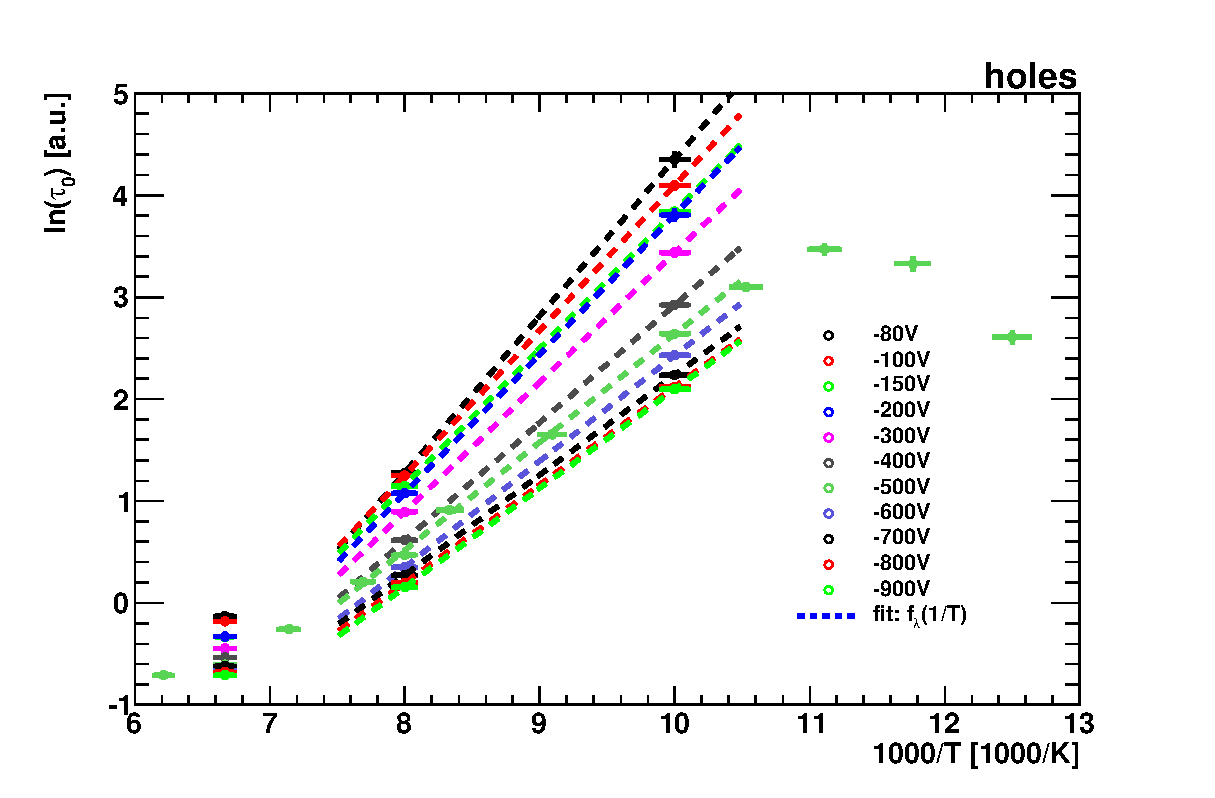
\includegraphics[width=0.49\textwidth]{figures/logtauvsTinvU_h}\put(-190,110){(B)}
 \caption{The fitted shape constant is shown as $\ln{(\tauzero)}$ versus the inverse temperature for various voltages including their corresponding linear fits extracting the activation energy. }
 \label{fig:fittauV}
\end{figure}

\subsection{Transit time}
\label{sec:tt}

\begin{figure}[t]
 \centering
 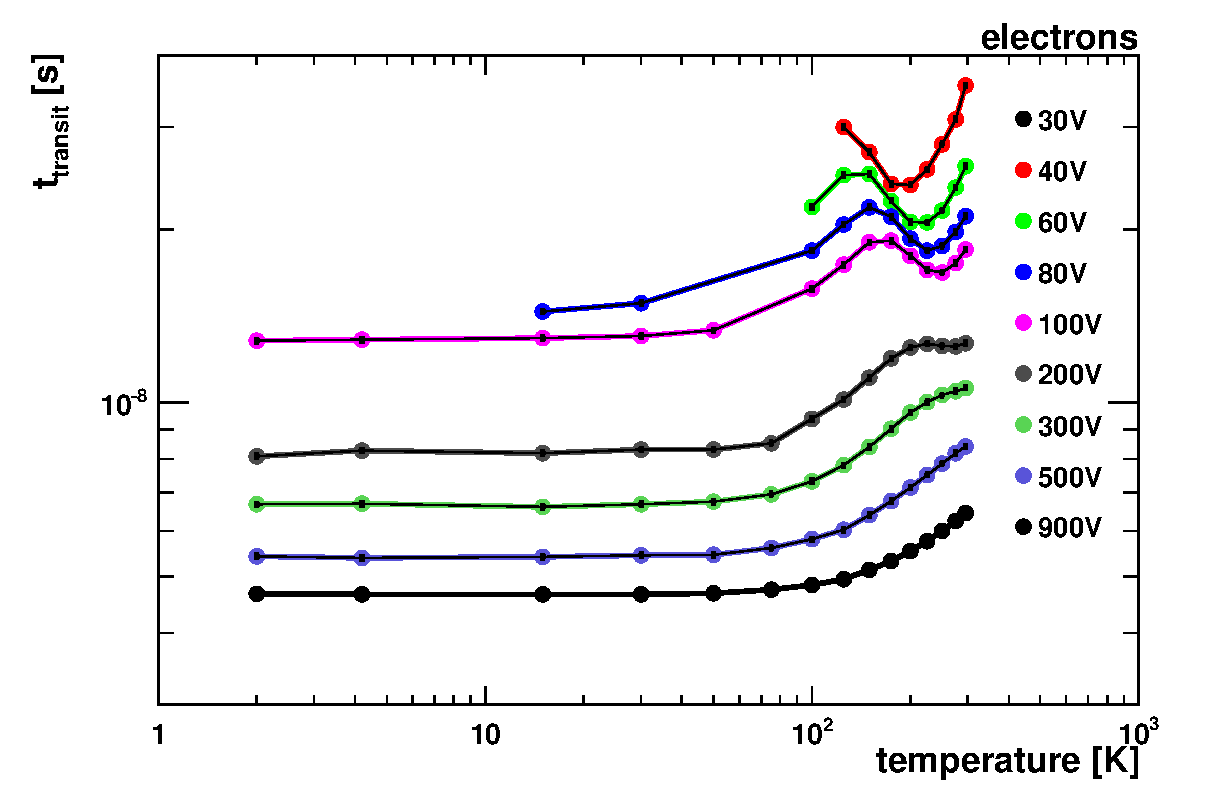
\includegraphics[width=0.49\textwidth]{figures/ttloglog_e.eps}\put(-190,110){(A)}
 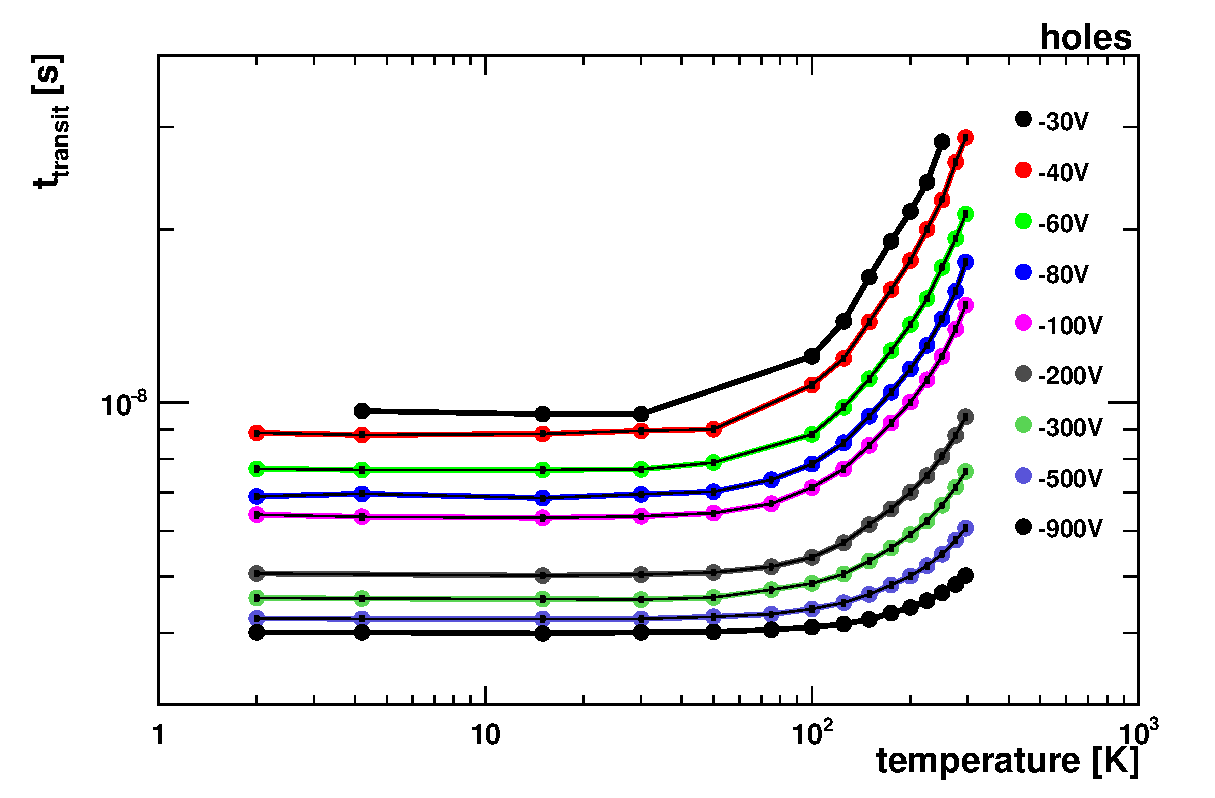
\includegraphics[width=0.49\textwidth]{figures/ttloglog_h.eps}\put(-190,110){(B)}
 

 \caption{The transit times for holes \textbf{(a)} and electrons \textbf{(b)} at various temperatures and fields are shown for \textit{S57}. 
Note the double logarithmic scale. Lines are drawn between measurements for constant voltages in order to guide the eye.}
 \label{fig:tt}
\end{figure}

The measured transit times are shown in Fig.~\ref{fig:tt} for \textit{S57} as an example. 
All three samples show the same behaviour. 
Transit times range from $\SI{3}{\nano\second}$ to $\SI{40}{\nano\second}$ for all fields and temperatures. 
Experimental sources of uncertainties affecting the measurement of the drift velocity are listed below including an estimate of their values.
\begin{itemize}
 \item[1)] The sample thickness has been measured with precision tools resulting in an uncertainty of the sample thickness below $<1\%$.
 \item[2)] The error in the measurement of the transit time $\sigma_{\ttr}$ depends on the ability to identify the rising and the falling edge, which in turn correlates with the SNR.
The SNR depends on the temperature and the electric field. 
$\sigma_{\ttr}$ is estimated as $\sigma_{\ttr} = \frac{\sigma_{\textrm{noise}}}{\textrm{slope}}$, with the baseline noise $sigma_{\textrm{noise}}$ and the maximum slope in the rising edge. 
At room temperature (low temperature) and $E\approx \SI{1}{\volt/\micro\meter}$, this approach leads to uncertainties of the transit time measurement of around $1\%$ ($2\%$),
 and up to $4\%$ at low temperature and low fields.
 \item[3)] At low SNRs the bandwidth limit was used in order to extent the accessible measurement range towards lower electric fields. 
The bandwidth limit leads to slower rising and falling edges. 
The effect on the transit time at $V_{\textrm{bias}} = \SI{100}{\volt}$ at RT is $\approx1\,\%$. 
At lower biases the rising/falling edges are slower, hence the effect is smaller. 
 \item[4)] Errors due to a possible non-uniformity of the electric field can be neglected, as a net-space charge seems to be absent in the tested samples.
 \item[5)] The uncertainty of the electric field strength is conservatively estimated to $1\%$.
 \item[6)] The uncertainty of the temperature measurement is about $1\%$. 
\end{itemize}




Figure~\ref{fig:tt} (a) shows how the transit time for holes increases with temperature over the entire temperature range,
 and how it decreases with increasing field over the whole field range. 
For electrons, Fig.~\ref{fig:tt} (b), the transit time decreases with increasing field, but does not monotonically increase for all biases. 
Only at high biases, down to $\SI{300}{\volt}$, the transit time increases with increasing temperature over the whole temperature range.
For smaller biases, a local maximum emerges, being more pronounced with decreasing bias.
The position of the local maximum shifts to lower temperatures with decreasing bias.
The abnormal behaviour of the electron transit time is likely to be caused by a re-population effect, a well-understood phenomenon in silicon \cite{Jacoboni197777}.
It was recently observed in high-purity scCVD diamond \cite{isberg:172103}, but at much lower temperatures and fields. 

 

\fi

%\newpage
\part{Modelling the experimental data}

\section{Discussion}
\label{sec:discussion}
\ifdefined\notFORPAPER

\subsection{Modelling the experimental data}

In this part the data described in part\,I is interpreted in a physical model and quantitatively formulated in a rate equation scheme.

It is a characteristic feature of the measured current pulse profiles in Fig.~\ref{fig:currentprofiles} that they are rectangular and practically constant a low temperature from 2\,K up to 70\,K at a given electric field. 
Above 70\,K the current amplitudes increase strongly showing rising and falling flanks reminiscent of an $\exp(-t/\tau(T))$-like behaviour with time constants $\tau(T)$ decreasing for higher temperatures. 
Evidently, the current profiles are composed of two different contributions one of which, at increasing temperatures, shows thermal activation.

\begin{figure}[tb]
 \centering
 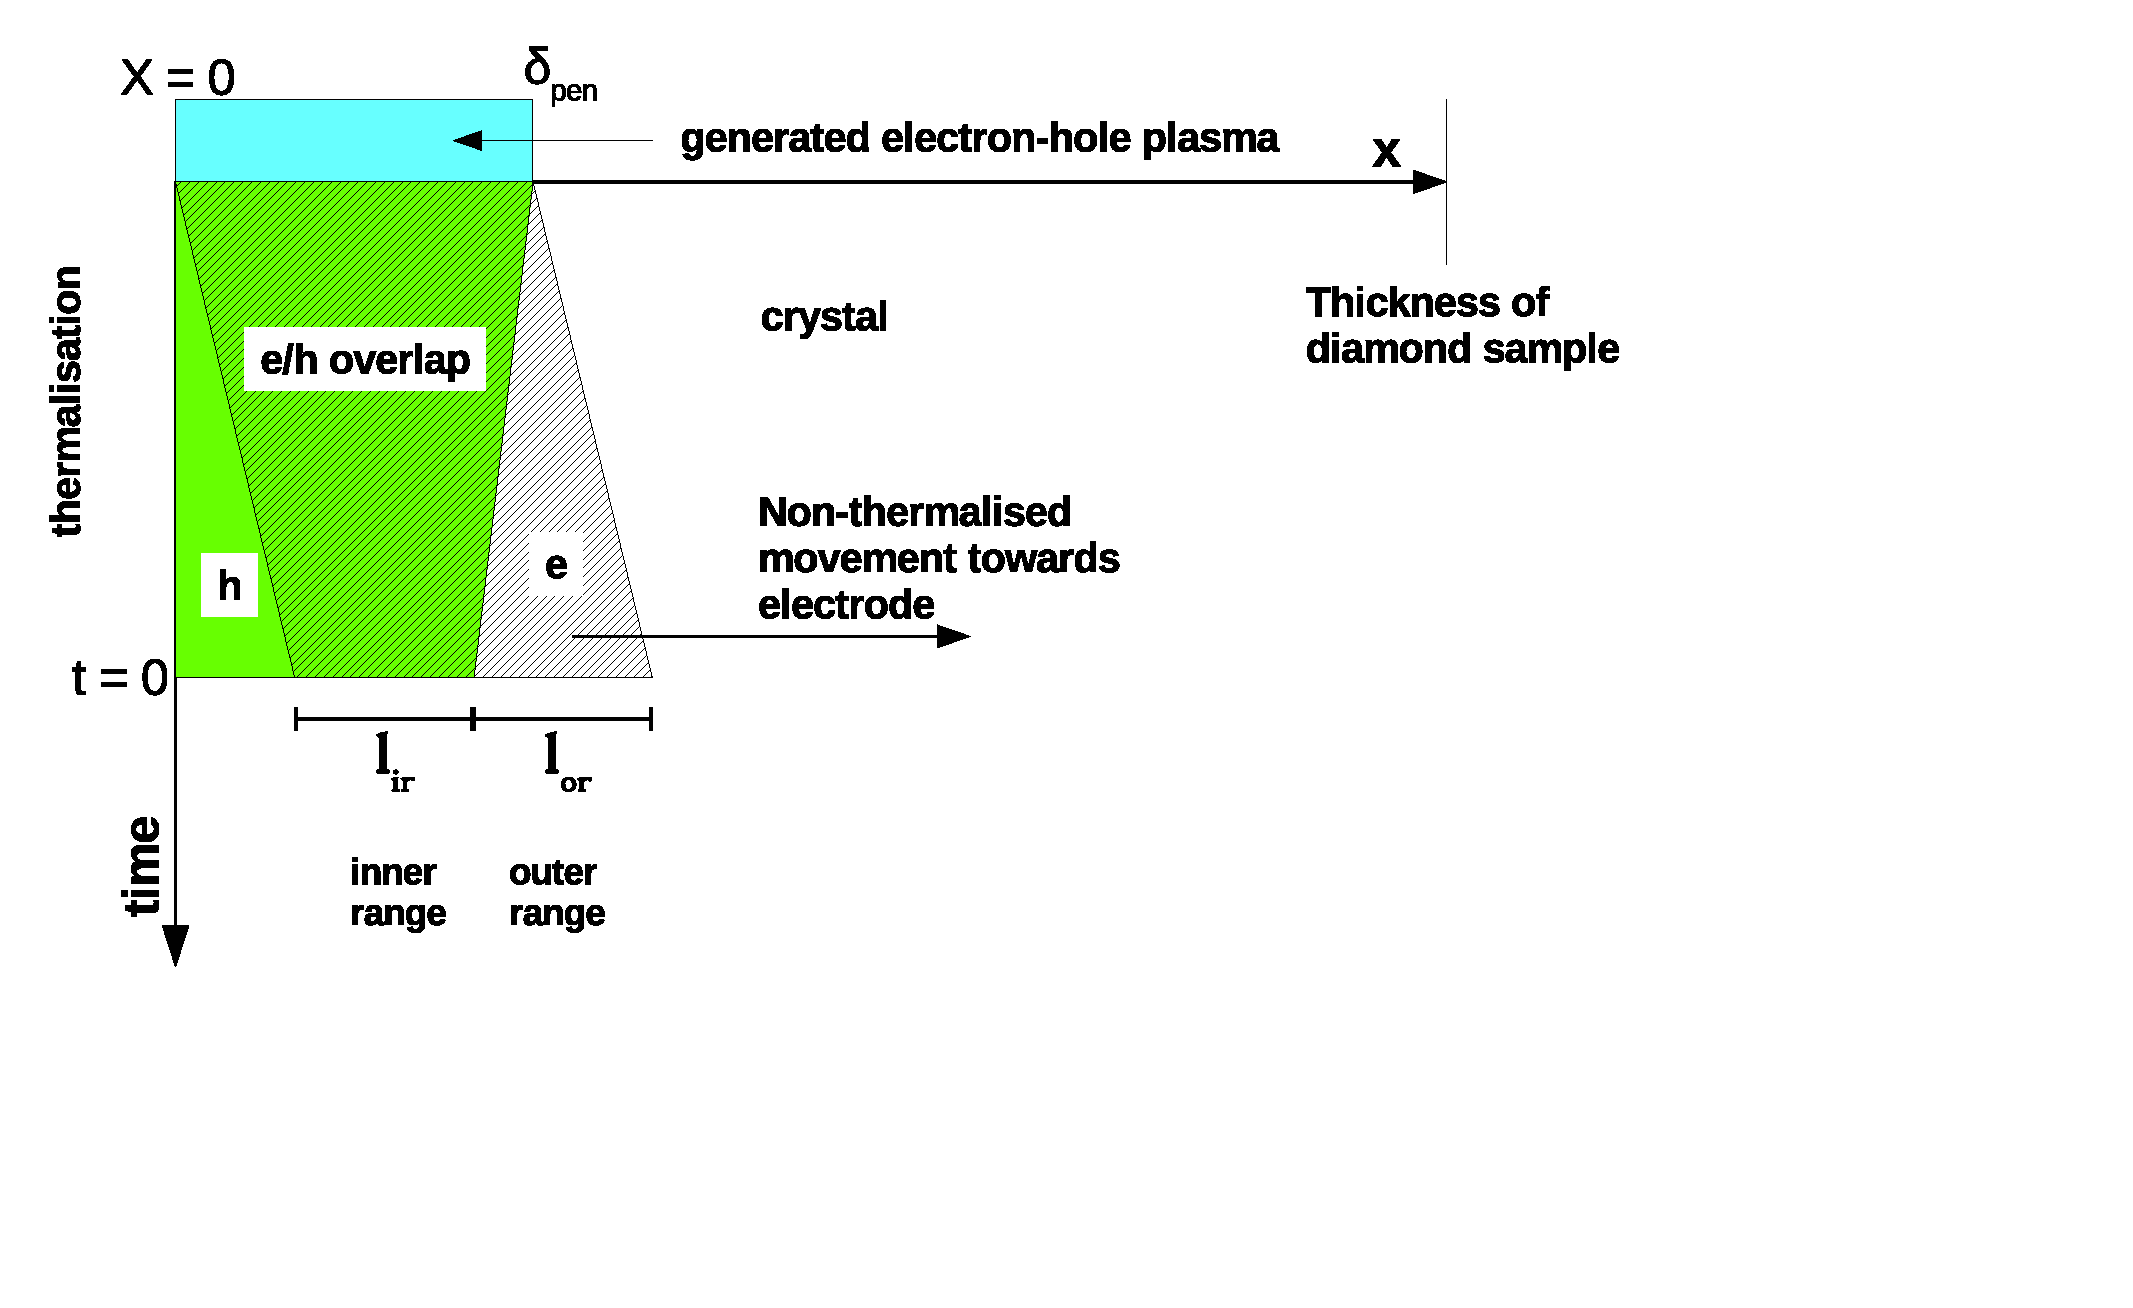
\includegraphics[trim=0 100 250 0, width=0.49\textwidth]{figures/non-therm.eps}\put(-30,30){(A)}
 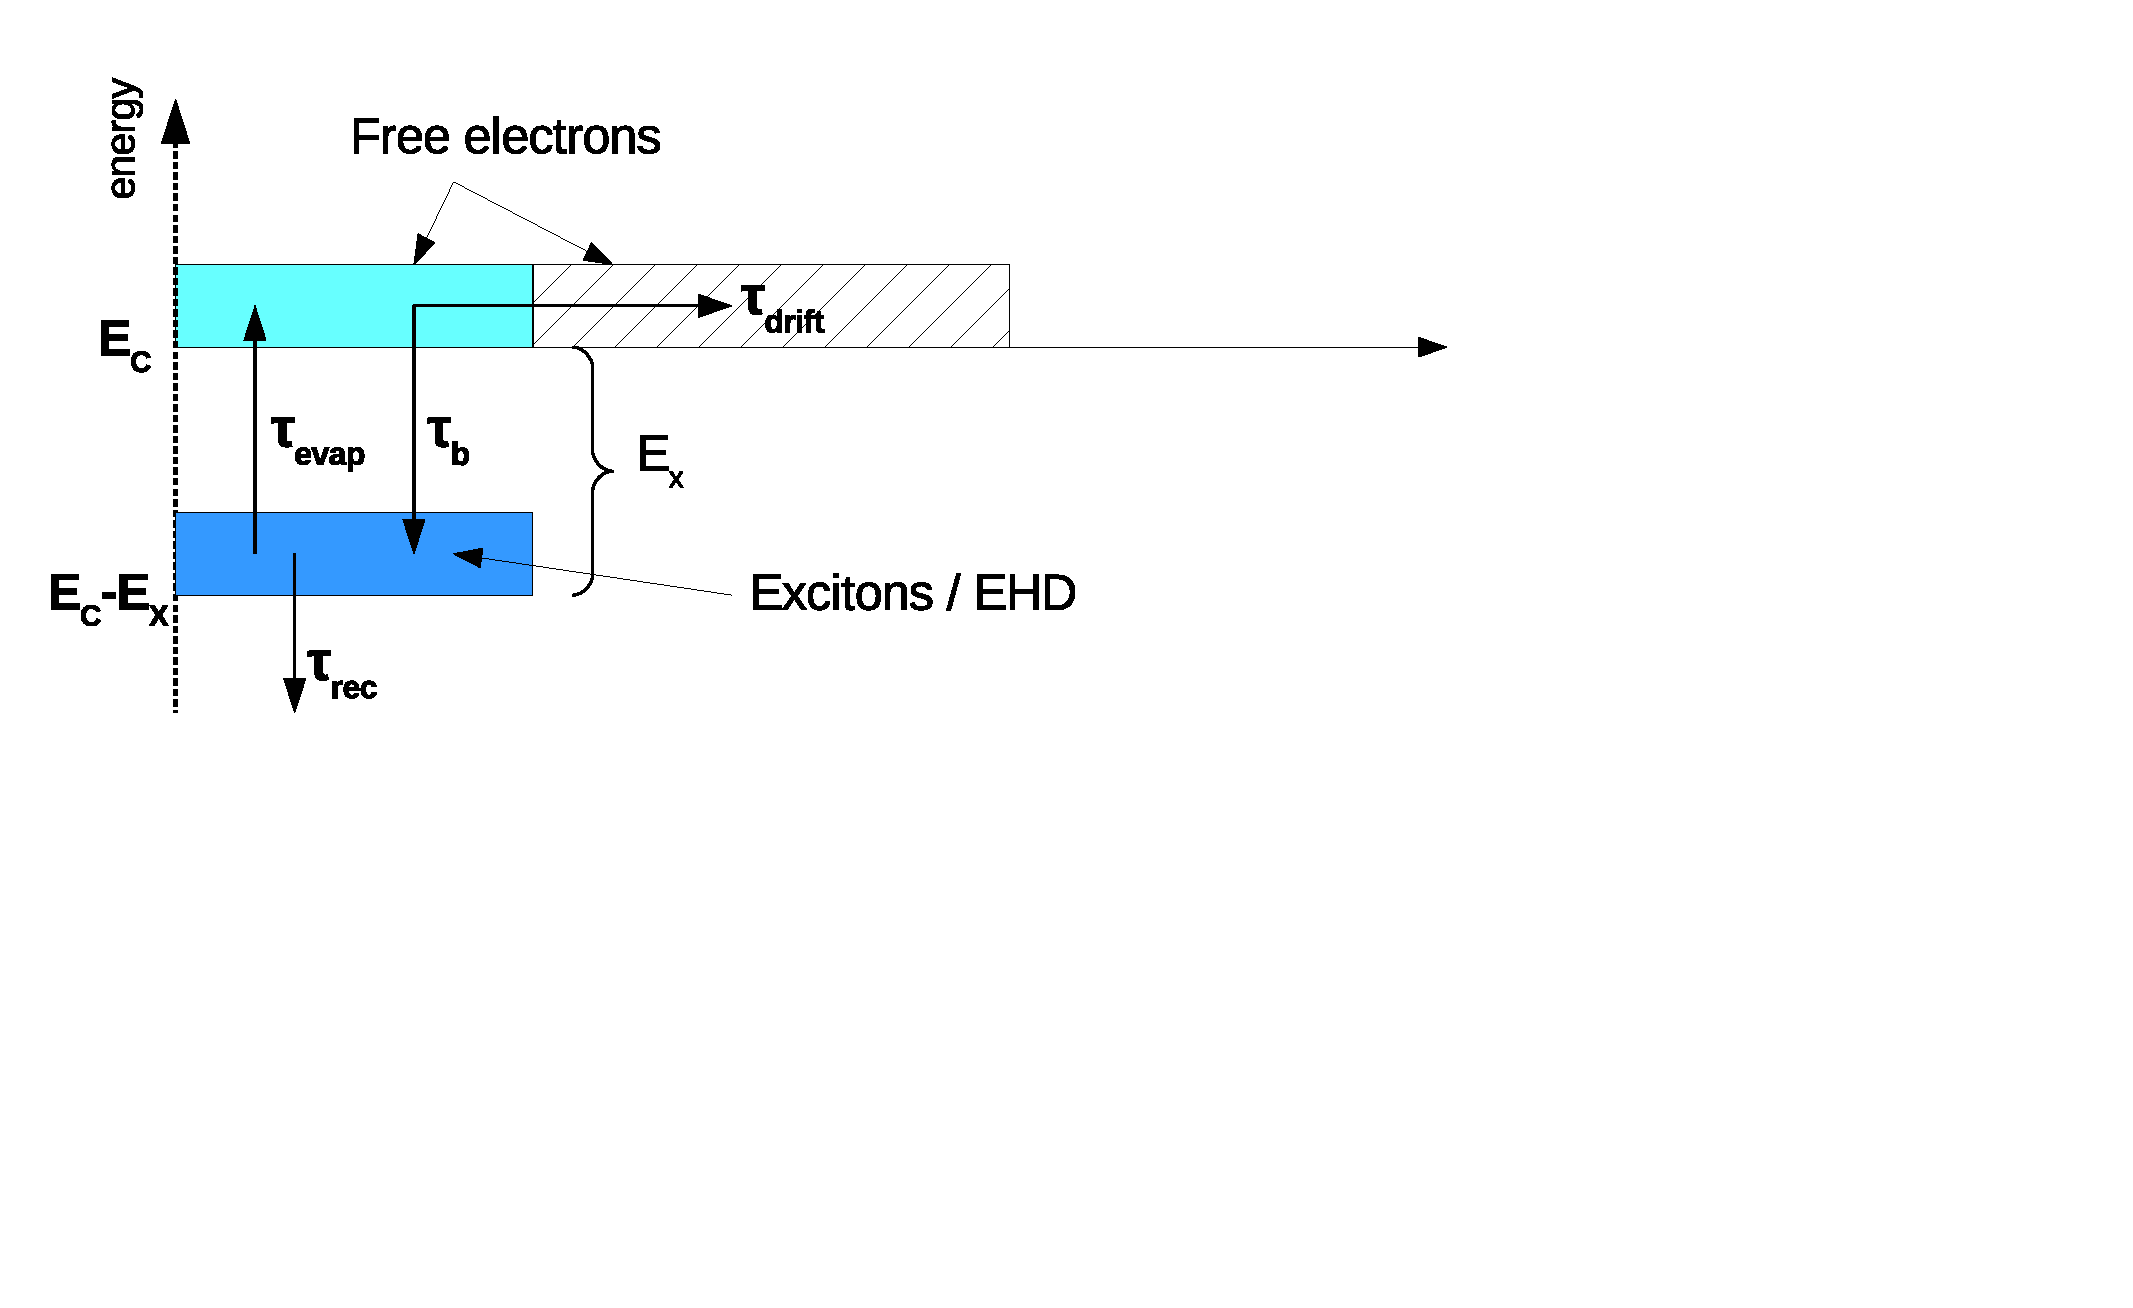
\includegraphics[trim=0 100 250 0, width=0.49\textwidth]{figures/NiveausTaus.eps} \put(-30,30){(B)} \\
 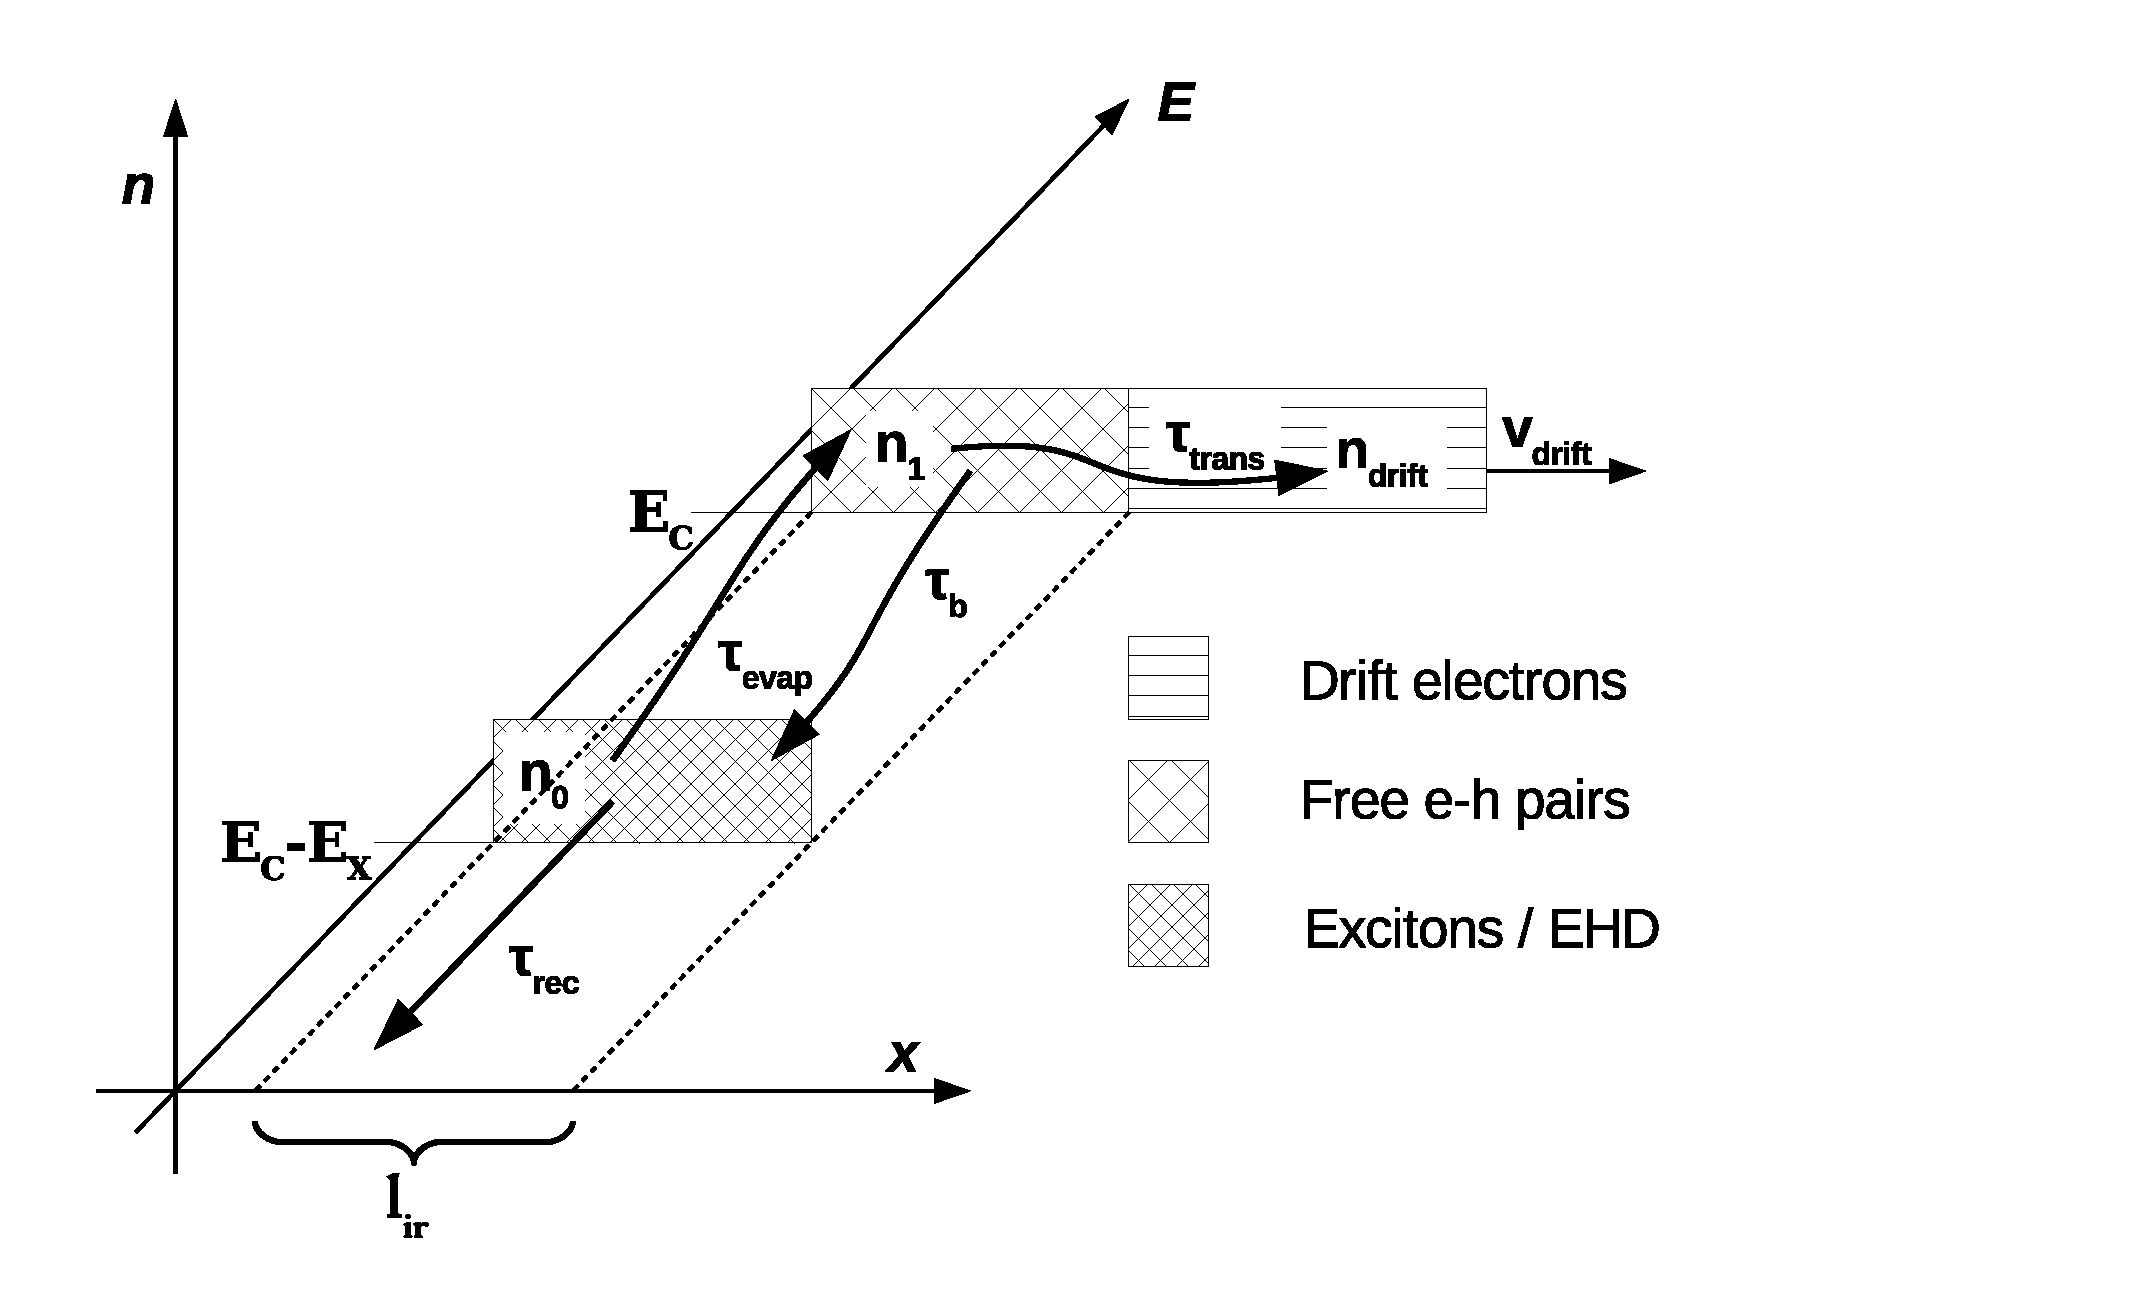
\includegraphics[trim=0  50 100 100, width=0.49\textwidth]{figures/NiveausTaus2.eps}\put(-30,30){(B')}

 \caption{(A) A sketch of the basic idea of the model with an inner and an outer region. 
 (B) The different energy levels and time constants are shown. 
 (B') Vorschlag einer anderen Version von (B), bei der die Dichte und Energie entlang unterschiedlicher Achsen dargestellt sind.}
 \label{fig:non-thermalised}
\end{figure}

The basic idea of the model as sketched in Fig.~\ref{fig:non-thermalised} (A) is the assumption that after the excitation of electrons and holes in highly excited band states
 there is a local separation of the two differently charged species during the relaxation phase under the influence of the electric field: 
 Electrons and holes drift in opposite directions separating locally from each other except for a central range where -  depending on the strength of the electric field  --  they still overlap. 
In this central overlap range, electrons and holes having reached their band edges after relaxation form a bound neutral charge-storage state no longer influenced by the electric field. 
However, this state can be thermally activated to yield a temperature-dependent current contribution. 
This is in contrast to the two outer regions which only contain electrons or holes inducing a temperature independent current. 
In the following, we will call these two ranges the inner and the outer range. 
The model neglects any charge carrier diffusion during relaxation and carrier transit. 
Therefore, it is one-dimensional and carriers move only in the direction perpendicular to the side facets of the $\SI{500}{\um}$ thick samples.

To derive a physical picture of the charge-storage state it is important to note that the temperature and electric field variations of the measured pulse profiles 
 are principally identical for electrons and holes {\color{red}(B1)}. 
We therefore conclude that the bound storage state must involve the two species in totally equivalent roles. 
There are only three types of electron-hole state that satisfy this condition:
 Free excitons (FE), excitons bound to neutral impurities such as donors or acceptors (BE), and electron-hole drops (EHD). 
The experimental part has shown that the activation energy is approximately 80\,meV at the most detailed studied electric field of $\SI{1}{\volt/\um}$ 
 (corresponding to an applied voltage of 500\,V) depending weakly on the electric field {\color{red}(B2)}. 
So, prior to a later more refined discussion, FEs with a binding energy of 80\,meV (Ref.   ) suggest themselves as the bound state in question. 
EHDs have binding energies in excess of the excitonic binding of 52...58\,meV (Ref.    ) significantly too much at the present status of the discussion {\color{red}(B3)}. 
BEs can definitely be excluded from further discussion: There is only one typical shallow impurity in diamond, the acceptor boron binding a hole with an ionization energy of\,370 meV. 
In this this neutral state boron can localize a FE with 55\,meV into a BE state. 
Though all diamonds contain small amounts of boron (often only detectable by sensitive luminescence analysis) our samples are yellowish indicating dominant doping with nitrogen,
 and the amount of boron would be far too low to govern the observed characteristic storage behaviour in which high carrier concentration up to $\SI{1e18}{\cm^{-3}}$ are involved. {\color{red}(B4)}
 

\subsubsection{Outer range}

For definiteness we discuss here the situation with electrons; holes can be treated completely analogously with parameter changes \textit{mutatis mutandis}.
The electron concentration in the outer range at the end of the relaxation phase is called $\No(0)$. 
The resulting current measured at the anode is

\begin{equation}
 j(t) = q\No(0)v(t)\quad {\color{red}(B5)}. 
\end{equation}

\noindent
The electron package reaches the anode at the transit time $t'$, from then the current decreases linearly to zero in a time interval of  $\Delta t = \dpen/v$  since the incoming carriers flow into the anode. 
Here $\dpen$ is the length of the initial ionisation volume at $t = 0$ (Fig.~\ref{fig:non-thermalised} (C)) and $v$ the applicable carrier velocity. 
Referring to the later discussion of possible values for these parameters we expect $\Delta t$ to lie in the picosecond range. 
This is too short to be experimentally resolved. 
The measured pulse profile is then simply rectangular with a duration of $\SI{500}{\um/v}$ and smeared edges due to scattering effects during the transit. 
For holes also rectangular current pulse profiles are measured and explained analogously.

\subsubsection{Inner range}

In the inner range the situation developed so far is modelled by a set of coupled rate equations following the intuitive sketch in Fig.~\ref{fig:non-thermalised}~(C). 
Prior to the formulation of the equations we describe the model in physical terms, referring to electrons in order to be specific.

The concentration of electrons bound in excitons in the inner range does not contribute to the measured current at low temperatures until the excitons are thermally dissociated at increasing temperatures. 
In the bound state, the electron concentration is denoted as $n_0$ and the electrons have an energy of -80\,meV relative to the conduction band edge at $\Ec = 0 $. 
During the excitonic binding, recombination can take place. 
We note in passing that even our highest fields are not able to tear off the excitons as a simple estimate shows. 
In the activated state, the electrons with concentration $n_1$ are free at energy $\Ec = 0 $ and can be extracted from the inner range by the electric field.
With these partial processes the rate equations read as 

\begin{align}
\label{math:diff1}
 \frac{\dd n_1}{\dd t} &= -\frac{n_1}{\tauone}  + \frac{n_0}{\tauevap} \qquad \textrm{with} \qquad\frac{1}{\tauone} = \frac{1}{\taub} + \frac{1}{\taudrift} \quad {\color{red}(B6)}\\
 \frac{\dd n_0}{\dd t} &= -\frac{n_0}{\tauzero} + \frac{n_1}{\taub} \qquad \textrm{with}    \qquad\frac{1}{\tauzero}= \frac{1}{\tauevap} + \frac{1}{\taurec} \quad {\color{red}(B7)}
 \label{math:diff2}
\end{align}

\noindent
The time constants are

\begin{itemize}
 \item $\tauone$: dwell time of $n_1$-electrons given by the competing loss processes of binding into excitons ($\taub$) and drift out of the inner range due to the electric field ($\taudrift$).
 \item $\tauzero$: lifetime of $n_0$-electrons (excitons)  given by the competing processes of exciton dissociation (or evaporation, $\tauevap$) and exciton recombination ($\taurec$).
\end{itemize}

\noindent
The drift time $\taudrift$ may be set equal to the extraction or depletion time of the inner range with extension $\lir$ as $\taudrift  = \lir/2v$,
 where the drift velocity $v$ depends on temperature and electric field. 

The set of rate equations (\ref{math:diff1}) and (\ref{math:diff2}) cannot be solved analytically. 
However, a simplification is possible so as to open a way for an analytical solution. 
The time $\taub$ describing the binding of $n_1$ electrons into excitons  may be expressed in the form

\begin{equation}
 \taub = 1/(\sigma \vth n_1) 
\end{equation}

\noindent
where $\sigma$ denotes the capture cross section for the binding into excitons, and $\vth$ is the average thermal velocity of the electrons. 
$\sigma$ can be calculated from the Bohr radius $r_x$ of the excitons, $\sigma  = 4 \pi {r_x}^2$  yielding with  $r_x = \SI{1.4}{\nm}$  as discussed in (Ref......)  a value $\sigma  \approx \SI{6e-14}{\cm^2}$,
 and $\vth = \sqrt{3\kB T/m\cdot\e }= \SI{1e7}{\cm/\s}$ at room temperature. 
Directly after relaxation, with an initial electron concentration of $n_1(0) = \SI{1e18}{\cm^{-3}}$ as estimated in the experimental part, $\taub$ is around 1.6\,ps,
 much shorter than $\tauevap = 1.2 \cdot \exp{80\,meV/\kB T}$ {\color{red}(B8)}.
The latter expression was derived from the experimental data:
 At high temperatures, $T \approx \SI{170}{\kelvin}$, it merges below 200\,ps, the experimental limit of resolution;
 at low temperatures, $T \approx \SI{100}{\kelvin}$, it goes over into the time constant $\taurec \approx  \SI{10}{\ns}$ of the competing parallel process of recombination. 
Hence, directly after exciton formation, $n_0(0) \gg   n_1(0)$ and $n_0(0) = \Nin(0)$ is practically equal to the whole inner electron concentration $\Nin(0)$. 

These considerations lead to the simplified equations

\begin{align}
\label{math:diff3}
 \frac{\dd n_1}{\dd t} &= -\frac{n_1}{\taudrift}  + \frac{n_0}{\tauevap},\quad {\color{red}(B9)}\\
 \frac{\dd n_0}{\dd t} &= -\frac{n_0}{\tauzero}.
 \label{math:diff4}
\end{align}

\noindent
The solution of (\ref{math:diff4}) is straight forward

\begin{equation}
 n_0(t) = n_0(0)\cdot \exp{\left(-t/\tauzero\right)}. 
\end{equation}

\noindent
The solution of (\ref{math:diff3}) is obtained as the solution of the homogeneous equation plus one particular solution of the inhomogeneous equation yielding

\begin{equation}
 n_1(t) = \left[ n_1(0) - \frac{\tauzero\taudrift}{\tauevap(\tauzero-\taudrift)} n_0(0)\right]\cdot \exp{\left(-t/\taudrift\right)} 
                        + \frac{\tauzero\taudrift}{\tauevap(\tauzero-\taudrift)} n_0(0) \cdot \exp{\left(-t/\tauzero\right)}
  \label{math:sol1}
\end{equation}

\noindent
The depletion of the inner range by electron drift is according to equation (\ref{math:diff3})

\begin{equation}
 \frac{\dd n_1}{\dd t}{}_{\big|_{\drift}} = + \frac{n_1(t)}{\taudrift} \equiv \frac{\dd \ndrift (t)}{\dd t}
\end{equation}

Here, the positive sign has to be taken as we are concerned with the electron concentration on the drift stretch lacking in the inner range.
The current released from the inner range to the drift stretch after integration of $\ndrift$ becomes {\color{red}(B10)}

\begin{equation}
 j(t) = \q \ndrift(t) v(t) = \q v(t) n_0(0) \cdot \frac{\tauzero}{\tauevap(\tauzero-\taudrift)} \cdot \Big[ -\taudrift\big( 1- \exp{(-t/\taudrift)}\big) + \tauzero\big( 1 - \exp{(t/\tauzero)} \big) \Big],
\end{equation}

\noindent
where $n_1(0) \ll n_0(0)$ has been neglected. 
$\taudrift = \lir/(2v)$ takes values from 67\,ps to 170\,ps for typical electric fields of $\SI{1.4}{\volt/\um}$ to $\SI{0.2}{\volt/\um}$, respectively. 
$\tauevap$ in comparison is much larger for $T \leq \SI{200}{\kelvin}$. 
These values of $\tauevap$ are not essentially changed when recombination times of the order of a few nanoseconds are included in $\tauevap$. 
Therefore, the first term in the brackets can be neglected yielding an approximate drift current of {\color{red}(B11)}

\begin{equation}
 j(t) =  \q n_1(0)v(t) \frac{\tauzero^2}{\tauevap(\tauzero-\taudrift)} \big( 1- \exp{(-t/\tauzero)}\big).
\end{equation}

This is in fact the pulse profile which we measure as the temperature-activated current contribution. 
The rising flank in the experiments corresponds to the term in brackets, and the asymptotic current value reflects complete electron depletion of the inner range. 
The pre-factor containing various time constants has the character of a supply efficiency limiting the current subject to the recombination time. 
When all restrictions of the time constants apply which were discussed, the pre-factor simplifies to unity. 
The falling flank of the pulse is given by an exponential $\exp(-t/\tau(T))$ as experimentally observed.

The total {\color{red}(B12)} incoming charge $Q$ measured at the anode is the integral of the drift current from $t = 0$ to $t= t'$

\begin{align}
 \Qin &= \q v \Nin(0) \frac{\tauzero^2}{\tauevap(\tauzero-\taudrift)} \cdot \Big[ t' - \tauzero \big( 1- \exp{(-t'/\tauzero)}\big) \Big] \\
   &= \q \Nin(0) \frac{\tauzero^2}{\tauevap(\tauzero-\taudrift)} \Big[  \SI{500}{\um} - v\tauzero \big( 1- \exp{(-t'/\tauzero)}\big) \Big] {\color{red}(B13)}
\end{align}

\noindent
and for $t = 0$ to $t = \infty$ (a few time constants) [jetzt mit $1/d$]

\begin{align}
 \Qin &= \q v/d \cdot \Nin(0) \frac{\tauzero^2}{\tauevap(\tauzero-\taudrift)} \cdot \Big[ t' \Big] \\
   &= \q \Nin(0) \frac{\tauzero^2}{\tauevap(\tauzero-\taudrift)}
\end{align}

\noindent
after insertion of the transit time $t´ =  \SI{500}{\um/v}$.
The first term in brackets, together with the pre-factors,
 corresponds to the total charge which was initially in the inner range and is entirely extracted for high enough temperatures to activate all electrons from there. 
The second term describes the loss out of the total charge due to those electrons which were not thermally activated at low temperatures remaining in the inner range and finally recombining there. 

\subsubsection{Total charge {\color{red}(B14)}}
Combining the inner and the outer currents and integrating to $t = t'$, we obtain

\begin{align}
 \Qtot &= \Qo(0) + Q_1(0) + Q_0(0) \frac{\tauzero}{\tauevap}\left[ 1 - \frac{\tauzero}{t'}(1 - \exp(-t'/\tauzero)) \right]\\ 
 &\approx \Qo(0) + \Qin(0) \frac{\tauzero}{\tauevap}\left[ 1 - \frac{\tauzero}{t'}(1 - \exp(-t'/\tauzero)) \right]
 \label{math:Q}
\end{align}

\noindent
and again for integration to $t = \infty$
\begin{equation}
 \Qtot = \Qo(0) + Q_1(0) + Q_0(0) \frac{\tauzero}{\tauevap}.
\end{equation}

\noindent
Assuming $Q_1(0)$ to be negligible and hence $Q_0(0) \approx \Qin(0)$, we obtain

\begin{equation}
 \Qtot = \Qo(0) + \Qin \frac{\tauzero}{\tauevap} = \Qo(0) + \Qin(0) \frac{1}{1+\frac{\tauevap}{\taurec}} = \Qo(0) + \Qin(0) \frac{1}{1+\frac{t_{e,0}}{\taurec}\cdot \exppEa}. 
 \label{math:Q2}
\end{equation}

\noindent
The expressions (\ref{math:Q}) and (\ref{math:Q2}) were used in Fig.~\ref{fig:QT} to fit the experimentally measured charge at the electrode, cf.\ also Eqs.~)\ref{eq:fitQinfty}) and ~(\ref{eq:fitQtprime}),
 and the agreement is very satisfactory for both electrons and holes. 


\subsection{Dependence of the activation energy $\Ea$ on the electric field}

Most of the experiments were initially performed at an electric field  $\xi = \SI{1}{\volt/\um}$ (applied voltage 500\,V) yielding an ample set of data points for $Q(T)$, c.f.\ Fig.~\ref{fig:QT}. 
In the course of the work $Q(T)$ was also measured for other field strengths extending from $\SI{0.2}{\volt/\um}$ (voltage 100\,V) to $\SI{1.8}{\volt/\um}$ (voltage 900\,V). 
Fits of eq. (\ref{math:Q}) {\color{red}(B15)} to these cases showed that the thermal activation energy $\Ea$ depends on $\xi$, decreasing weakly for $\xi \geq \SI{1}{\volt/\um}$
 and increasing in succession more strongly towards lower field strengths, cf.\ Fig.~\ref{fig:Eafield}. 
This result casts doubts on our initial conclusion that the charge storage state in the inner range consists of FEs {\color{red}(B16)}. 
An approximate free-hand extrapolation to $\xi = 0$ yields a value of $\Ea$ between 125\,meV and 140\,meV.

\begin{figure}[tb]
 \centering
 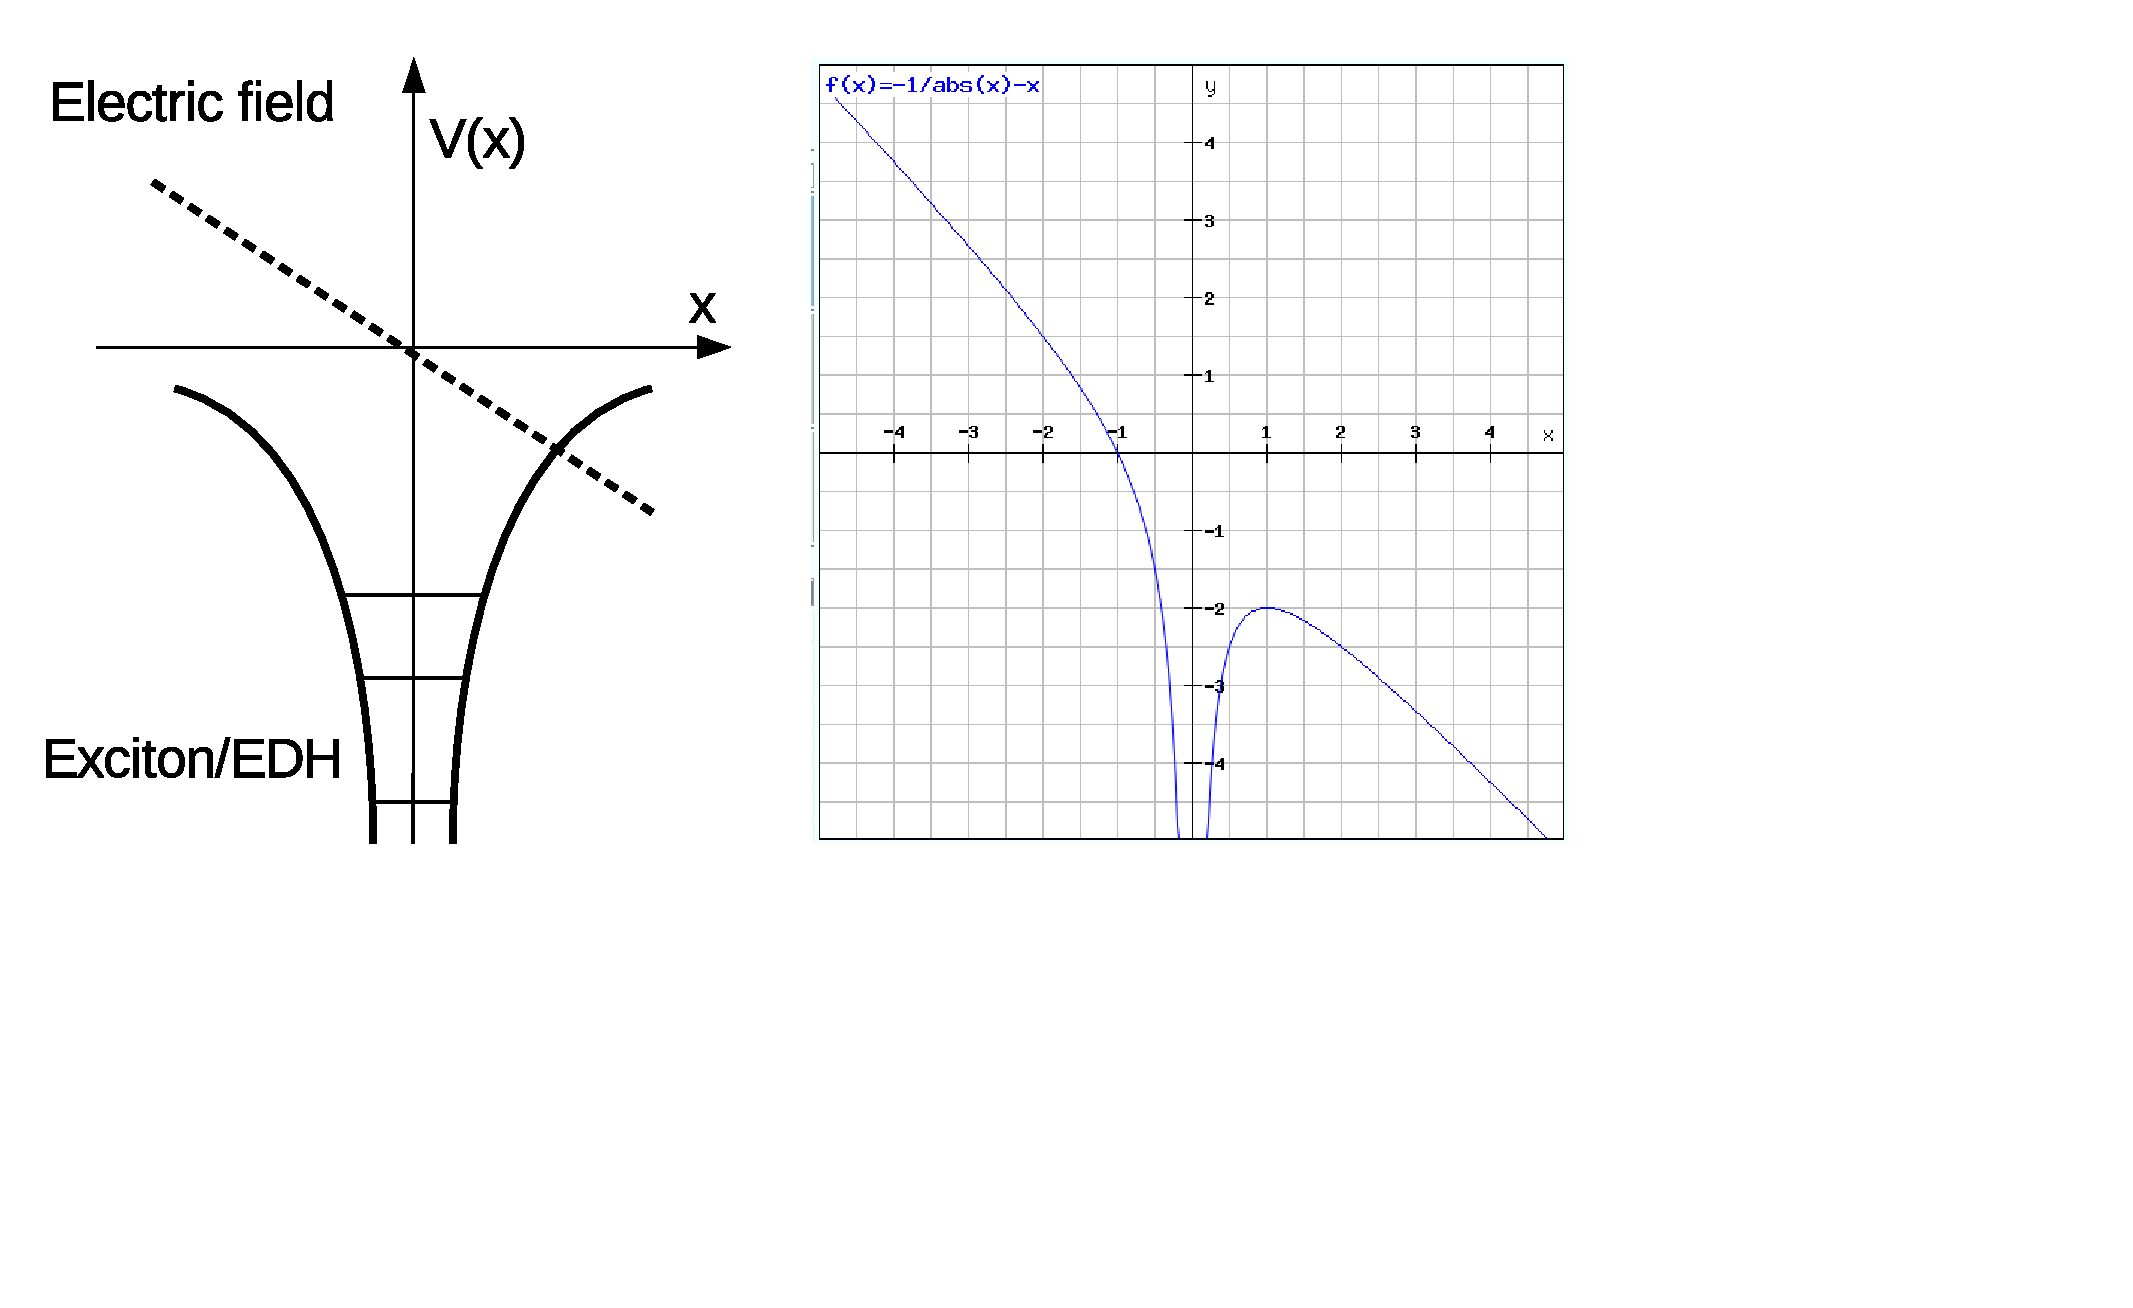
\includegraphics[trim=0 170 0 0, width=0.8\textwidth]{figures/ExcField.eps}
 \caption{(A) The electric potential for a FE and the externally applied voltage are shown separately. (B) The combination of a linearly decreasing field with a hydrogenic potential of the FE. 
 [Fuer rechts zeichne ich noch ein schoeneres Bild.]}
 \label{fig:excfield}
\end{figure} 

As discussed earlier, defects if considered as storage states must bind electrons and holes in an equivalent way. 
Above, we have argued that boron, the only shallow and typical impurity in diamond, must be discarded as a centre to bind FEs into BEs. 
The only alternative satisfying the condition of equivalent electron-hole binding are EHDs. 
In EHDs the additional electron-hole binding in excess of the FE binding amounts to 52...58\,meV (Ref.     ) so that a total binding energy of
 $\Ea = (80 + 52..58)\,\si{\milli\eV}$ would result in good agreement with our rough estimate. 
The phase diagram of FE gas and EHD liquid has been studied recently in detail, and it has been found that the critical temperature $\Tc$ up to which EHDs can exist is 173\,K. 
At this temperature, in our experiments nearly all electrons from the storage state have been thermally dissociated. 
We conclude that for the whole temperature range in the electron charge collection measurements {\color{red}(B17)} one unique activation energy $\Ea$ does apply. 
Also, none of the restrictions made in the deduction of the expressions (9) above is violated by invoking EHDs in addition to FEs  in the activation process.

(Der Absatz ist m.M.n.\ wichtig, um zu argumentieren, dass die Aktivierungsenergie durchaus mehr als 80\,meV sein kann. Deswegen wuerde ich den Absatz beibehalten.)
It remains to be discussed whether the excitation is strong enough to create EHDs. 
The original excitation strength by the incoming $\alpha$-particles is very high amounting to $\SI{1e21}{\cm^{-3}}$ e-h pairs in a pulse {\color{red}(B18)}. 
Following literature data, it might be assumed that the charge carriers do not slowly diffuse but are pushed away from the excitation region by the phonons which they create in their relaxation
 from the high-energy states down to the conduction or valence band edges, respectively. 
In the literature, this driving force is called phonon wind (Ref.   ). 
A simple estimate not reported here shows that – if the phonons would travel isotropically in space from their excitation region
 -- the e-h concentration would decrease dramatically within a relaxation time of 0.1 to 1 ps down to a value where no EHD formation is possible. 
However, it is well known (Ref.        ) that the phonons travel in anisotropic,
 strongly focused channels creating a phonon caustic due to the fact that the directions of their $k$-vectors and their energy flow are not collinear. 
The generated e-h plasma is thought to be driven in such narrow local channels during the relaxation process, that the electrons are strongly scattered out of the channels by carrier-carrier interaction
 and impurity-assisted scattering so that their concentration after relaxation would be by far sufficiently high to condensate into EHDs.

\begin{figure}[tb]
 \centering
 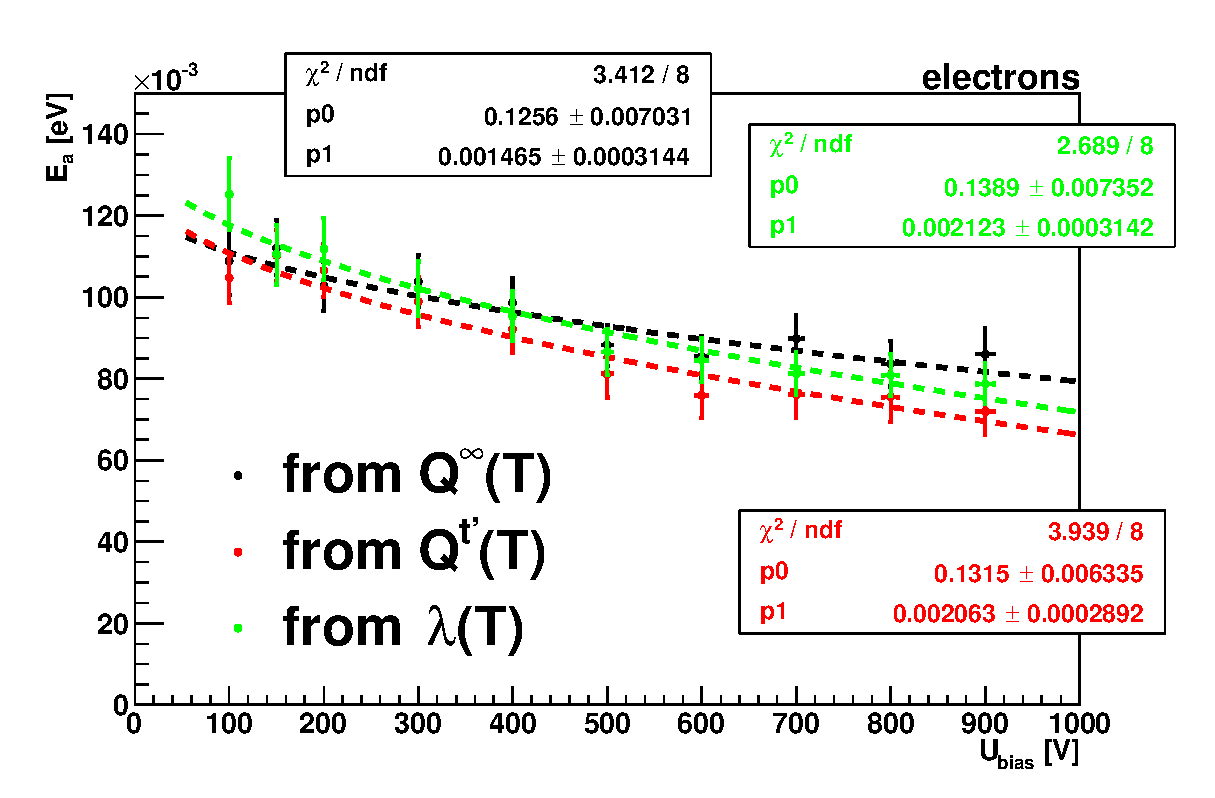
\includegraphics[trim=0 0 0 0, width=0.49\textwidth]{figures/EaU_e.eps}
 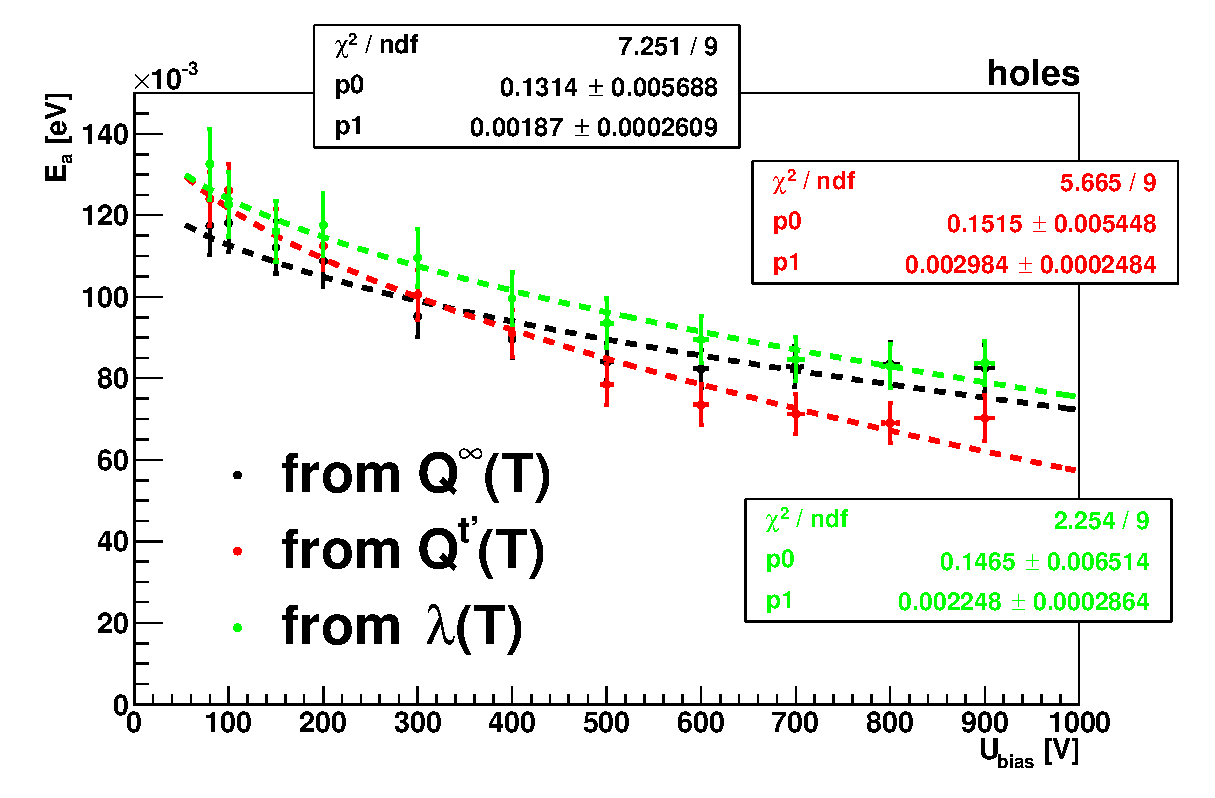
\includegraphics[trim=0 0 0 0, width=0.49\textwidth]{figures/EaU_h.eps}
 \caption{The activation energy as obtained from $Q(T,E)$ and $\lambda(T,E)$ are plotted as a function of the electric field. 
 Fit-functions are overlaid and discussed in section~\ref{sec:discussion}. [Anm.: Die Statistikboxen kommen spaeter noch weg oder werden schoener gemacht.]}
 \label{fig:Eafield}
\end{figure} 

To come to a quantitative expression for $\Ea(\xi)$, we discuss the e-h binding potential in an electric field (Fig.\ref{fig:excfield}). 
The sum of the excitonic Coulomb potential, $V = -\e^2 / (4\pi\varepsilon\varepsilon_0 x)$ and the superposed electric field potential, $V = -\e\xi x$ is asymmetric
 with a local maximum at $x_{\textrm{max}} = \e / \sqrt{4\pi\varepsilon\varepsilon_0 \xi}$ {\color{red}(B18')}
 lowered in comparison to the ionization limit of FEs by $\Delta E(x_{\textrm{max}}) = -2\e^2 ( \xi / \sqrt{4\pi\varepsilon\varepsilon_0 \e} )$. 
This reduces the ionization energy of the FEs {\color{red}(B19)} to a value 
 
\begin{equation}
 \Ea(\xi) = \Ea(0) - \Delta E(\xi) = \Ea(0) - \e\cdot \frac{2\e}{ \sqrt{4\pi\varepsilon\varepsilon_0 \e d} } \cdot\sqrt{U}
 \label{math:delta}
\end{equation}

\noindent
The pre-factor $\frac{2\e}{ \sqrt{4\pi\varepsilon\varepsilon_0 \e d} } = \SI{1.4e-3}{\sqrt{\volt}}$ can be compared to a fit of the form $\Ea - C\cdot\sqrt{U}$,
 resulting in pre-factors of about $\SI{2.0(3)}{\sqrt{\volt}}$, which is in reasonable agreement with the model. 

The envelope function of FEs is hydrogen-like having s-like even symmetry. 
Therefore, the envelope function will not cause any splitting or shift in the electric field of p-like odd symmetry.
However, there are additional non-hydrogenic degrees of freedom in the FEs:
 The electron $\Gamma6$ state splits twofold  in an electric field due to the lifting of the orientational degeneracy (“valley-orbit splitting”), and the hole $\Gamma8$ state also splits into two. 
The total fourfold splitting cannot quantitatively be calculated due to the lack of values for the electric compliance constants. 
We estimate, however, that in diamond these effects are negligible even at our highest fields of $\SI{1.8}{\volt/\um}$ not exceeding a few meV.
Fits to the experimental activation energies in Fig.~\ref{fig:Eafield} have been made using eq.\ (\ref{math:delta}) with $\Ea(0)$ as a free fit parameter. 
Results are presented superimposed on the experimental data in Fig.~\ref{fig:Eafield} showing good agreement for $\Ea(0) = \SI{130}{\milli\eV}$. 
This value is fully compatible with a binding energy of (80 + 52..58)\,meV for EHDs being the storage state in our experiments.



\subsection{Dependence of the collected charge on the electric field}

\subsubsection{Low-temperature case}

At low temperature, $T = \SI{2}{\kelvin}$, the collected charge is exclusively provided by the outer range. 
The data points lie well on a straight line up to the highest field value $\xi = \SI{1.8}{\volt/\um}$, cf.~Fig.~\ref{fig:QvsE}. 
This applies analogously to holes. 
In the model, the electron concentration available for the drift at t = 0 in the outer range depends on the electric field which has separated electrons and holes during the relaxation. 
If the drift velocities in this process are independent of the electric field (in contrast to the band edge velocities)
 the extension of the outer range $x_\e$ would be linear as a function of the field and with it the electron concentration and the collected charge. 
As mentioned at the outset of the paper (SOLLTE AM ANFANG VON PART II ERWAEHNT WERDEN), no literature data on drift velocities in highly excited electron or hole states have been found to document this case. 
Extrapolation of our data points to higher fields delivers an intersection with the curve for the total collected charge measured at $T = \SI{295}{\kelvin}$ at $\xi = \SI{4.5}{\volt/\um}$. 
In the model, this hypothetical value characterizes the case where electrons and holes have been completely separated by the field in the relaxation process leaving no inner overlap range,
 hence $x_\e + x_\h = \SI{10}{\um}$. 
Assuming in this crude estimate equal velocities for electrons and holes, we have $x_\e = \SI{5}{\um} = \vrelax \taurelax$. 
For an assumed relaxation time of $\taurelax$ in the order of 0.1\,ns a drift velocity of $\SI{5e6}{\cm/\s}$ follows comparable to the range of drift values at the band edges at medium fields. 
This gives us confidence that the model also in this respect is physically realistic although it cannot be further documented.

\subsubsection{High-temperature case}

{\color{red}(B28')}
We discuss the data for the highest experimental temperature, $T = \SI{295}{\kelvin}$, and low electric fields. 
This case is not covered by the rate equations since $\tauevap \leq \taudrift$, and electrons thermally activated from $n_0$ are not totally extracted from the inner range. 
Therefore, $n_1$ increases and the earlier made simplifications are no longer valid. 
However, a different approach can be made to describe the collected charge in this case.
When $n_1$ increases, $\taub$ decreases by virtue of $\taub = 1/ (\sigma \vth n_1)$ leading to a quasi-equilibrium of $n_1$ and $n_0$,
 since the loss processes drift ($\taudrift$) and recombination ($\taurec$) are only small in comparison to the carrier re-distribution rates given by $\taub$ and $\tauevap$. 
It is then irrelevant which of the two states suffers the loss. 
We may define a “charge collection efficiency” as the ratio of the desired drift rate to the total loss rate

\begin{equation}
 Q / Q_0 = R_\drift / (R_\drift + R_\textrm{rec}) = \frac{1/\taudrift}{1/\taudrift + 1/\taurec} = \frac{\taurec}{\taurec + \taudrift}.
\end{equation}

\noindent
With $\taudrift = \lir/2v = \lir/2\mu_\e\xi$ we obtain

\begin{equation}
 Q(\xi) / Q_0 = \frac{2\mu_\e \xi \taurec}{l + 2\mu_\e\xi\taurec}.
\end{equation}

\noindent
Low-field values for $\mu_\e$ are contained in the figures...  of (Ref. {\color{red}(B29)}), $\mu_\e = \SI{1150}{\cm^2/\volt\s}$, and $l = \SI{10}{\um}$ so that 

\begin{equation}
 Q(\xi) / Q_0 = \SI{2300}{\cm^2/\volt\s} \xi \taurec / \left( \SI{10}{\um} + \SI{2300}{\cm^2/\volt\s} \xi \taurec \right).
\end{equation}

\noindent
This expression describes approximately the observed drop of $Q(\xi)$ for $T = \SI{295}{\kelvin}$ and low fields for a recombination time close to $\taurec = \SI{14}{\ns}$.

% \subsection{Recombination time}
% The recombination time can be readily extracted from data for temperatures between 100 and 125\,K.


\subsection{Valley re-population effects}

The transit time $\ttr$ of electrons was measured versus temperature for electric fields from
 $\xi = \SI{0.08}{\volt/\um}$ (applied voltage 40\,V) to $\xi = \SI{1.8}{\volt/\um}$ (applied voltage 900\,V) (Fig.~\ref{fig:tt}). 
At high fields $\ttr$ is small and constant up to 100\,K, and then increases due to electron scattering by phonons. 
The transit time is larger for lower applied voltages and, beginning at 300\,V, successively more pronounced maxima for voltages down to 40\,V are observed
 which appear systematically shifted towards lower temperatures. 
We ascribe this effect to a 'valley re-population' between ``fast'' and ``slow'' electrons in the electric field. 

\begin{figure}[tb]
 \centering
 \includegraphics[trim=0 0 50 0, width=0.49\textwidth]{figures/f-scat.eps}
 \includegraphics[trim=0 0 50 0, width=0.49\textwidth]{figures/degenerated-states.eps}
 \caption{Shown are the six CBM valleys, which -- under the influence of an electric field -- are two-fold degenerated in the [100] direction and four-fold degenerated in the perpendicular plane. 
 An energy difference $\delta$ characterises the splitting due to the different mass-factors in the dispersion relation. }
 \label{fig:gamma6}
\end{figure}

To explain this effect, we show in Fig.~\ref{fig:gamma6} the orientational valley-orbit splitting of $\Gamma6$ electrons in a homogeneous electric field. 
The electron state splits into two states, one at lower energy with twofold degeneracy for electrons in conduction band valleys parallel to the field direction in $k$-space,
 and the other at higher energy with fourfold degeneracy for electrons in conduction band valleys perpendicular to the field in $k$-space. 
The terms parallel and perpendicular refer to the long  ($\ml$) and short ($\mt$) axes of the valley ellipsoids of constant energy in $k$-space. 
This situation was exhaustively sketched and described in (Ref. \cite{lofas:032139}).

Taking the expression $\mu = \q \tauscat / \mestar$ 
 and assuming equal band scattering times $\tauscat$ in the two substates electrons in the lower state move slowly as their associated effective mass is $\ml = 1.4 \cdot m_0$ 
while electrons in the upper state move fast having a much smaller effective mass $\mt = 0.36\cdot m_0$.

Our situation is different from that studied by Gabrysch et al.\ (Ref.~\cite{isberg:172103,valley,gabrysch:063719} under similar experimental conditions. %FIXME check refs
Their samples are ultra-pure showing extremely little scattering between electrons in the two split substates. 
This enabled them to register the current pulses due to fast and slow electrons individually at different arrival times when reaching the anode. 
From these fascinating experiments they could deduce a firm value for the mass ratio $R = \ml/\mt = 5$. 
This is a much more reliable value than earlier data obtained by less direct methods. 
Such previous values were discussed in Ref.\ ?? and were found as cited above yielding $R = \ml /\mt = 3.9$. 
Our present samples are yellowish {\color{red}(B20)}
 indicating a rather high concentration of nitrogen (deep) donors and possibly other defects causing high scattering rates between the two split states. 
We call the effect which we observe “valley re-population” among the two states,
 and comparison with the samples used by Gabrysch et al.\ demonstrates that it must be induced by impurity-assisted intervalley scattering.

We discuss impurity-assisted scattering in more detail. 
In diamond, the valleys are centred in $k$-space at 0.76 \% of the Brillouin zone at $2\pi/a_0$  in  [100]-type directions. 
Re-population of the two inequivalent parallel and perpendicular valleys means f-type intervalley scattering (IVS) by phonons with suitable wave-vectors $k\, ||\,  [110]$  in $k$-space. 
In a pure crystal, IVS depends on the availability of phonons satisfying the wave-vector and energy conservation rules as well.  
Phonons which can scatter must therefore gap a wave-vector difference of $\Delta k = \sqrt{2}\cdot 0.76 (2\pi/a_0) = 1.07 (2\pi/a_0)$. 
In the  [110]-direction, this is nearly exactly the full length of the Brillouin zone from $k = 0$ ($Γ$-point) to the $K$-point. 
The minimum energy needed for a phonon with this $k$-value is 95\,meV according to the phonon dispersion curves (Ref.\ ??). 
Selection rules may impose further restrictive conditions. 
Unless the two substates are split by this amount there will be no IVS.  
Actually, the electrons have kinetic energy in their valleys so that the cited values of $\Delta k$ and the minimum phonon energy have to be slightly reconciled. 
The samples of the present study contain a significant concentration of defects (e.g.\ nitrogen is a deep donor-like defect) which can take up $k$-vectors
 by virtue of their wave function which is widely spread in $k$-space. 
This invalidates the $k$-conservation rule and enables re-population of the electrons at any splitting.

Experimental proof of impurity-assisted IVS has previously been demonstrated in silicon. 
There, FE and EHD luminescence was studied under uniaxial stress splitting the electron states completely analogously to an electric field,
 and “hot” and “cold” recombination lines were observed due to the electrons in the split upper or lower energy valleys, respectively. 
When the crystals were pure there was no thermalisation of the hot luminescence line at all until the splitting energy reached the TA-phonon energy
 at the adequate scattering wave-vektor $\Delta k\,||\, [110]$ setting then the valley populations into quasi-thermal equilibrium. 
For moderately increased doping with donors or acceptors the hot luminescence line disappeared in succession faster at much lower stress and could no more be observed for high doping levels.

Our present situation can be modelled in a straight forward simple way:  
For strong scattering the population ratio of the two states can be written as a Boltzmann factor in quasi-thermal equilibrium
 
\begin{equation}
 \frac{\nt}{\nl} = \frac{4}{2}\exp{(-\delta/\kB T)}
\end{equation}

\noindent
with the splitting energy $\delta$ and {\color{red}(B21)}

\begin{equation}
 \nt = \frac{N}{1+2\exp{(-\delta/\kB T)}}, \qquad  \nl = \frac{N}{1+1/2\exp{(-\delta/\kB T)}},
\end{equation}

\noindent
where $N = \nt + \nl$ is the concentration of electrons in both states. 
The total current amounts to  {\color{red}(B22)}

\begin{equation}
 j = j_{\textrm{t}} + j_{\textrm{l}} = \q\left( \nt \vt + \nl \vl \right) = \q N \xi \left( \frac{\mut}{1+2\exp{(-\delta/\kB T)}}  + \frac{\mul}{1+1/2\exp{(+\delta/\kB T)}}\right) 
\end{equation}

\noindent
using $v_{\textrm{t/l}} = \mu_{\textrm{t/l}}\xi$. 
After some reformulation {\color{red}(B23)} we find for the transit time

\begin{equation}
 t' = \frac{d}{\mul\xi}\cdot \frac{1}{ \dfrac{1}{1+2\exp{(-\delta/\kB T)}}\cdot(1-R) + R} \quad {\color{red}(B23')}.
 \label{math:tprime}
\end{equation}

We have still to associate the splitting energies $\delta$ with the applied voltages. 
To this sake it is important to note that $\delta$ is not primarily due to an electrostatic splitting which is estimated to amount to only a few meV at the highest field strengths. 
Owing to lacking literature data on the electric compliance constants we cannot calculate such values. 
Instead, we are concerned with a dynamic splitting due to the kinetic energy of the electrons when moving in the two states. 
With $E_{\textrm{kin,t/l}} = 1/2 m_{\e,\textrm{t/l}}v_{\textrm{t/l}}^2$, we find {\color{red}(B24)}

\begin{equation}
 \delta = \Delta E_{\textrm{kin}} = 1/2 \cdot\ml \vl^2 - 1/2 \cdot\mt \vt^2.
\end{equation}

\noindent
Using the above cited mass ratio $R =5$ results in

\begin{equation}
 \delta = 2 \ml \vl^2
\end{equation}

\noindent
There is no accurate analytic expression for $\vdrift$ as a function of $\xi$ or the applied voltage,
 but numerical values $\vdrift(\xi)$ can be extracted from experimental data in reference \cite{jansen:173706} in Fig.~5 (b). 
Some values are explicitly quoted in table~\ref{tab:deltas} {\color{red}(B25)}.
In this compilation, a value of $\ml  = 1.36\,m_0$  was used {\color{red}(B26)}.

\begin{table}[t]
\caption[delta values]{Compilation of extracted values of $\vdrift$ and $\delta$.}
 \begin{center}
  \begin{tabular}{c|c|c||c|c|c||c|c}
  voltage $U$ & $\vdrift$ & $\delta$ & v at RT& v(225\,K) & v(150\,K) & $\delta$ (150\,K) & $\vl$(150\,K)\\
  $[\si{\volt}]$  & $[10^4\,\si{\m/\s}]$  & $[\si{\meV}]$  &  $[10^6\,\si{\cm/\s}]$ &  & & $[\si{\meV}]$  & $[10^4\,\si{\m/\s}]$\\ \hline
  40  &      &       & 1.5  & 2.1 &  1.9 & &\\
  60  & 3.2  &  15.8 & 2.0  & 2.5 &  2.1 &   1.0 &  0.58\\
  80  & 4.0  &  24.7 & 2.5  & 2.9 &  2.3 & &  \\
  100 & 4.6  &  32.6 & 2.8  & 3.1 &  2.7 &   1.7 &  0.75\\
  150 & 5.9  &  53.8 & 3.6  & 3.6 &  3.8 & &  \\
  200 & 7.0  &  75.7 & 4.2  & 4.2 &  4.8 &   5.9 &  1.4\\
  300 &      &       & 5.0  & 5.3 &  6.3 &  11.6 &  1.9\\
  400 & 9.5  & 139.0 & 5.6  & 6.3 &  7.4 & 165   &  7.3\\
  500 & 10.2 & 160.2 & 6.3  & 7.0 &  8.3 & 212   &  8.3\\
  900 &      &       & 8.2  & 9.2 & 10.3 & 328   & 10.3\\
  \end{tabular}
  \label{tab:deltas}
 \end{center}
\end{table}

\begin{figure}[tb]
 \centering
 \includegraphics[trim=0 150 0 0, width=0.80\textwidth]{figures/dummy_repop.eps}
 \caption{Siehe Anmerkungen {\color{red}(B27)}}
 \label{fig:repop}
\end{figure}


For the model curves represented in Fig.~\ref{fig:repop}  the transit time was taken in the alternative form {\color{red}(B27)}

\begin{equation}
 t' = \frac{\SI{500}{\um}}{\vl}\frac{1+2\exp{(-\delta/\kB T)}}{1+10\exp{(-\delta/\kB T)}} \equiv \frac{\SI{500}{\um}}{v_{\textrm{eff}}}
\end{equation}

\noindent
following from equation (\ref{math:tprime}) after inserting $R = 5$, and $\vl$ was numerically associated with the applied voltages according to table~\ref{tab:deltas}.
To account for the basic phonon scattering as a function of temperature underlying all experimental curves in Fig.~\ref{fig:tt}, we have employed the entirely empirical expression {\color{red}(B28)}

\begin{equation}
 t_{\textrm{basic}} = \left( 4.3 - \num{0.6e-4}\,T + \num{2.2e-5}\,T^2 \right) \cdot \frac{500}{U} ^{\left( 0.5 + \frac{0.6}{300\,T} \right)} \textrm{ in nanoseconds}.
\end{equation}

\noindent
Comparison of these model curves with the measured curves (Fig.~\ref{fig:repop}) {\color{red}(B27)} shows that the model reproduces all relevant characteristic aspects in a convincing way. 
In detail, however, there is no satisfactory quantitative agreement. 
This may be due to the mass value chosen, deviations from a parabolic band dispersion which we have tacitly implied by the form of the kinetic energy and which can become crucial for the high energies involved,
 neglect of the static splitting of the substates, or numerical uncertainties in the listing given above.



\else

\subsection{Modelling the experimental data}

In this part the data described in part\,I is interpreted in a physical model and quantitatively formulated in a rate equation scheme.

It is a characteristic feature of the measured current pulse profiles in Fig.~\ref{fig:currentprofiles} that they are rectangular and practically constant a low temperature from 2\,K up to 70\,K at a given electric field. 
Above 70\,K the current amplitudes increase strongly showing rising and falling flanks reminiscent of an $\exp(-t/\tau(T))$-like behaviour with time constants $\tau(T)$ decreasing for higher temperatures. 
Evidently, the current profiles are composed of two different contributions one of which, at increasing temperatures, shows thermal activation.

\begin{figure}[tb]
 \centering
 \includegraphics[trim=0 100 250 0, width=0.49\textwidth]{figures/non-therm.eps}\put(-30,30){(A)}
 \includegraphics[trim=0 100 250 0, width=0.49\textwidth]{figures/NiveausTaus.eps} \put(-30,30){(B)} \\
 \includegraphics[trim=0  50 100 100, width=0.49\textwidth]{figures/NiveausTaus2.eps}\put(-30,30){(B')}

 \caption{(A) A sketch of the basic idea of the model with an inner and an outer region. 
 (B) The different energy levels and time constants are shown. 
 (B') Vorschlag einer anderen Version von (B), bei der die Dichte und Energie entlang unterschiedlicher Achsen dargestellt sind.}
 \label{fig:non-thermalised}
\end{figure}

The basic idea of the model as sketched in Fig.~\ref{fig:non-thermalised} (A) is the assumption that after the excitation of electrons and holes in highly excited band states
 there is a local separation of the two differently charged species during the relaxation phase under the influence of the electric field: 
 Electrons and holes drift in opposite directions separating locally from each other except for a central range where -  depending on the strength of the electric field  --  they still overlap. 
In this central overlap range, electrons and holes having reached their band edges after relaxation form a bound neutral charge-storage state no longer influenced by the electric field. 
However, this state can be thermally activated to yield a temperature-dependent current contribution. 
This is in contrast to the two outer regions which only contain electrons or holes inducing a temperature independent current. 
In the following, we will call these two ranges the inner and the outer range. 
The model neglects any charge carrier diffusion during relaxation and carrier transit. 
Therefore, it is one-dimensional and carriers move only in the direction perpendicular to the side facets of the $\SI{500}{\um}$ thick samples.

To derive a physical picture of the charge-storage state it is important to note that the temperature and electric field variations of the measured pulse profiles 
 are principally identical for electrons and holes {\color{red}(B1)}. 
We therefore conclude that the bound storage state must involve the two species in totally equivalent roles. 
There are only three types of electron-hole state that satisfy this condition:
 Free excitons (FE), excitons bound to neutral impurities such as donors or acceptors (BE), and electron-hole drops (EHD). 
The experimental part has shown that the activation energy is approximately 80\,meV at the most detailed studied electric field of $\SI{1}{\volt/\um}$ 
 (corresponding to an applied voltage of 500\,V) depending weakly on the electric field {\color{red}(B2)}. 
So, prior to a later more refined discussion, FEs with a binding energy of 80\,meV (Ref.   ) suggest themselves as the bound state in question. 
EHDs have binding energies in excess of the excitonic binding of 52...58\,meV (Ref.    ) significantly too much at the present status of the discussion {\color{red}(B3)}. 
BEs can definitely be excluded from further discussion: There is only one typical shallow impurity in diamond, the acceptor boron binding a hole with an ionization energy of\,370 meV. 
In this this neutral state boron can localize a FE with 55\,meV into a BE state. 
Though all diamonds contain small amounts of boron (often only detectable by sensitive luminescence analysis) our samples are yellowish indicating dominant doping with nitrogen,
 and the amount of boron would be far too low to govern the observed characteristic storage behaviour in which high carrier concentration up to $\SI{1e18}{\cm^{-3}}$ are involved. {\color{red}(B4)}
 

\subsubsection{Outer range}

For definiteness we discuss here the situation with electrons; holes can be treated completely analogously with parameter changes \textit{mutatis mutandis}.
The electron concentration in the outer range at the end of the relaxation phase is called $\No(0)$. 
The resulting current measured at the anode is

\begin{equation}
 j(t) = q\No(0)v(t)\quad {\color{red}(B5)}. 
\end{equation}

\noindent
The electron package reaches the anode at the transit time $t'$, from then the current decreases linearly to zero in a time interval of  $\Delta t = \dpen/v$  since the incoming carriers flow into the anode. 
Here $\dpen$ is the length of the initial ionisation volume at $t = 0$ (Fig.~\ref{fig:non-thermalised} (C)) and $v$ the applicable carrier velocity. 
Referring to the later discussion of possible values for these parameters we expect $\Delta t$ to lie in the picosecond range. 
This is too short to be experimentally resolved. 
The measured pulse profile is then simply rectangular with a duration of $\SI{500}{\um/v}$ and smeared edges due to scattering effects during the transit. 
For holes also rectangular current pulse profiles are measured and explained analogously.

\subsubsection{Inner range}

In the inner range the situation developed so far is modelled by a set of coupled rate equations following the intuitive sketch in Fig.~\ref{fig:non-thermalised}~(C). 
Prior to the formulation of the equations we describe the model in physical terms, referring to electrons in order to be specific.

The concentration of electrons bound in excitons in the inner range does not contribute to the measured current at low temperatures until the excitons are thermally dissociated at increasing temperatures. 
In the bound state, the electron concentration is denoted as $n_0$ and the electrons have an energy of -80\,meV relative to the conduction band edge at $\Ec = 0 $. 
During the excitonic binding, recombination can take place. 
We note in passing that even our highest fields are not able to tear off the excitons as a simple estimate shows. 
In the activated state, the electrons with concentration $n_1$ are free at energy $\Ec = 0 $ and can be extracted from the inner range by the electric field.
With these partial processes the rate equations read as 

\begin{align}
\label{math:diff1}
 \frac{\dd n_1}{\dd t} &= -\frac{n_1}{\tauone}  + \frac{n_0}{\tauevap} \qquad \textrm{with} \qquad\frac{1}{\tauone} = \frac{1}{\taub} + \frac{1}{\taudrift} \quad {\color{red}(B6)}\\
 \frac{\dd n_0}{\dd t} &= -\frac{n_0}{\tauzero} + \frac{n_1}{\taub} \qquad \textrm{with}    \qquad\frac{1}{\tauzero}= \frac{1}{\tauevap} + \frac{1}{\taurec} \quad {\color{red}(B7)}
 \label{math:diff2}
\end{align}

\noindent
The time constants are

\begin{itemize}
 \item $\tauone$: dwell time of $n_1$-electrons given by the competing loss processes of binding into excitons ($\taub$) and drift out of the inner range due to the electric field ($\taudrift$).
 \item $\tauzero$: lifetime of $n_0$-electrons (excitons)  given by the competing processes of exciton dissociation (or evaporation, $\tauevap$) and exciton recombination ($\taurec$).
\end{itemize}

\noindent
The drift time $\taudrift$ may be set equal to the extraction or depletion time of the inner range with extension $\lir$ as $\taudrift  = \lir/2v$,
 where the drift velocity $v$ depends on temperature and electric field. 

The set of rate equations (\ref{math:diff1}) and (\ref{math:diff2}) cannot be solved analytically. 
However, a simplification is possible so as to open a way for an analytical solution. 
The time $\taub$ describing the binding of $n_1$ electrons into excitons  may be expressed in the form

\begin{equation}
 \taub = 1/(\sigma \vth n_1) 
\end{equation}

\noindent
where $\sigma$ denotes the capture cross section for the binding into excitons, and $\vth$ is the average thermal velocity of the electrons. 
$\sigma$ can be calculated from the Bohr radius $r_x$ of the excitons, $\sigma  = 4 \pi {r_x}^2$  yielding with  $r_x = \SI{1.4}{\nm}$  as discussed in (Ref......)  a value $\sigma  \approx \SI{6e-14}{\cm^2}$,
 and $\vth = \sqrt{3\kB T/m\cdot\e }= \SI{1e7}{\cm/\s}$ at room temperature. 
Directly after relaxation, with an initial electron concentration of $n_1(0) = \SI{1e18}{\cm^{-3}}$ as estimated in the experimental part, $\taub$ is around 1.6\,ps,
 much shorter than $\tauevap = 1.2 \cdot \exp{80\,meV/\kB T}$ {\color{red}(B8)}.
The latter expression was derived from the experimental data:
 At high temperatures, $T \approx \SI{170}{\kelvin}$, it merges below 200\,ps, the experimental limit of resolution;
 at low temperatures, $T \approx \SI{100}{\kelvin}$, it goes over into the time constant $\taurec \approx  \SI{10}{\ns}$ of the competing parallel process of recombination. 
Hence, directly after exciton formation, $n_0(0) \gg   n_1(0)$ and $n_0(0) = \Nin(0)$ is practically equal to the whole inner electron concentration $\Nin(0)$. 

These considerations lead to the simplified equations

\begin{align}
\label{math:diff3}
 \frac{\dd n_1}{\dd t} &= -\frac{n_1}{\taudrift}  + \frac{n_0}{\tauevap},\quad {\color{red}(B9)}\\
 \frac{\dd n_0}{\dd t} &= -\frac{n_0}{\tauzero}.
 \label{math:diff4}
\end{align}

\noindent
The solution of (\ref{math:diff4}) is straight forward

\begin{equation}
 n_0(t) = n_0(0)\cdot \exp{\left(-t/\tauzero\right)}. 
\end{equation}

\noindent
The solution of (\ref{math:diff3}) is obtained as the solution of the homogeneous equation plus one particular solution of the inhomogeneous equation yielding

\begin{equation}
 n_1(t) = \left[ n_1(0) - \frac{\tauzero\taudrift}{\tauevap(\tauzero-\taudrift)} n_0(0)\right]\cdot \exp{\left(-t/\taudrift\right)} 
                        + \frac{\tauzero\taudrift}{\tauevap(\tauzero-\taudrift)} n_0(0) \cdot \exp{\left(-t/\tauzero\right)}
  \label{math:sol1}
\end{equation}

\noindent
The depletion of the inner range by electron drift is according to equation (\ref{math:diff3})

\begin{equation}
 \frac{\dd n_1}{\dd t}{}_{\big|_{\drift}} = + \frac{n_1(t)}{\taudrift} \equiv \frac{\dd \ndrift (t)}{\dd t}
\end{equation}

Here, the positive sign has to be taken as we are concerned with the electron concentration on the drift stretch lacking in the inner range.
The current released from the inner range to the drift stretch after integration of $\ndrift$ becomes {\color{red}(B10)}

\begin{equation}
 j(t) = \q \ndrift(t) v(t) = \q v(t) n_0(0) \cdot \frac{\tauzero}{\tauevap(\tauzero-\taudrift)} \cdot \Big[ -\taudrift\big( 1- \exp{(-t/\taudrift)}\big) + \tauzero\big( 1 - \exp{(t/\tauzero)} \big) \Big],
\end{equation}

\noindent
where $n_1(0) \ll n_0(0)$ has been neglected. 
$\taudrift = \lir/(2v)$ takes values from 67\,ps to 170\,ps for typical electric fields of $\SI{1.4}{\volt/\um}$ to $\SI{0.2}{\volt/\um}$, respectively. 
$\tauevap$ in comparison is much larger for $T \leq \SI{200}{\kelvin}$. 
These values of $\tauevap$ are not essentially changed when recombination times of the order of a few nanoseconds are included in $\tauevap$. 
Therefore, the first term in the brackets can be neglected yielding an approximate drift current of {\color{red}(B11)}

\begin{equation}
 j(t) =  \q n_1(0)v(t) \frac{\tauzero^2}{\tauevap(\tauzero-\taudrift)} \big( 1- \exp{(-t/\tauzero)}\big).
\end{equation}

This is in fact the pulse profile which we measure as the temperature-activated current contribution. 
The rising flank in the experiments corresponds to the term in brackets, and the asymptotic current value reflects complete electron depletion of the inner range. 
The pre-factor containing various time constants has the character of a supply efficiency limiting the current subject to the recombination time. 
When all restrictions of the time constants apply which were discussed, the pre-factor simplifies to unity. 
The falling flank of the pulse is given by an exponential $\exp(-t/\tau(T))$ as experimentally observed.

The total {\color{red}(B12)} incoming charge $Q$ measured at the anode is the integral of the drift current from $t = 0$ to $t= t'$

\begin{align}
 \Qin &= \q v \Nin(0) \frac{\tauzero^2}{\tauevap(\tauzero-\taudrift)} \cdot \Big[ t' - \tauzero \big( 1- \exp{(-t'/\tauzero)}\big) \Big] \\
   &= \q \Nin(0) \frac{\tauzero^2}{\tauevap(\tauzero-\taudrift)} \Big[  \SI{500}{\um} - v\tauzero \big( 1- \exp{(-t'/\tauzero)}\big) \Big] {\color{red}(B13)}
\end{align}

\noindent
and for $t = 0$ to $t = \infty$ (a few time constants) [jetzt mit $1/d$]

\begin{align}
 \Qin &= \q v/d \cdot \Nin(0) \frac{\tauzero^2}{\tauevap(\tauzero-\taudrift)} \cdot \Big[ t' \Big] \\
   &= \q \Nin(0) \frac{\tauzero^2}{\tauevap(\tauzero-\taudrift)}
\end{align}

\noindent
after insertion of the transit time $t´ =  \SI{500}{\um/v}$.
The first term in brackets, together with the pre-factors,
 corresponds to the total charge which was initially in the inner range and is entirely extracted for high enough temperatures to activate all electrons from there. 
The second term describes the loss out of the total charge due to those electrons which were not thermally activated at low temperatures remaining in the inner range and finally recombining there. 

\subsubsection{Total charge {\color{red}(B14)}}
Combining the inner and the outer currents and integrating to $t = t'$, we obtain

\begin{align}
 \Qtot &= \Qo(0) + Q_1(0) + Q_0(0) \frac{\tauzero}{\tauevap}\left[ 1 - \frac{\tauzero}{t'}(1 - \exp(-t'/\tauzero)) \right]\\ 
 &\approx \Qo(0) + \Qin(0) \frac{\tauzero}{\tauevap}\left[ 1 - \frac{\tauzero}{t'}(1 - \exp(-t'/\tauzero)) \right]
 \label{math:Q}
\end{align}

\noindent
and again for integration to $t = \infty$
\begin{equation}
 \Qtot = \Qo(0) + Q_1(0) + Q_0(0) \frac{\tauzero}{\tauevap}.
\end{equation}

\noindent
Assuming $Q_1(0)$ to be negligible and hence $Q_0(0) \approx \Qin(0)$, we obtain

\begin{equation}
 \Qtot = \Qo(0) + \Qin \frac{\tauzero}{\tauevap} = \Qo(0) + \Qin(0) \frac{1}{1+\frac{\tauevap}{\taurec}} = \Qo(0) + \Qin(0) \frac{1}{1+\frac{t_{e,0}}{\taurec}\cdot \exppEa}. 
 \label{math:Q2}
\end{equation}

\noindent
The expressions (\ref{math:Q}) and (\ref{math:Q2}) were used in Fig.~\ref{fig:QT} to fit the experimentally measured charge at the electrode, cf.\ also Eqs.~)\ref{eq:fitQinfty}) and ~(\ref{eq:fitQtprime}),
 and the agreement is very satisfactory for both electrons and holes. 


\subsection{Dependence of the activation energy $\Ea$ on the electric field}

Most of the experiments were initially performed at an electric field  $\xi = \SI{1}{\volt/\um}$ (applied voltage 500\,V) yielding an ample set of data points for $Q(T)$, c.f.\ Fig.~\ref{fig:QT}. 
In the course of the work $Q(T)$ was also measured for other field strengths extending from $\SI{0.2}{\volt/\um}$ (voltage 100\,V) to $\SI{1.8}{\volt/\um}$ (voltage 900\,V). 
Fits of eq. (\ref{math:Q}) {\color{red}(B15)} to these cases showed that the thermal activation energy $\Ea$ depends on $\xi$, decreasing weakly for $\xi \geq \SI{1}{\volt/\um}$
 and increasing in succession more strongly towards lower field strengths, cf.\ Fig.~\ref{fig:Eafield}. 
This result casts doubts on our initial conclusion that the charge storage state in the inner range consists of FEs {\color{red}(B16)}. 
An approximate free-hand extrapolation to $\xi = 0$ yields a value of $\Ea$ between 125\,meV and 140\,meV.

\begin{figure}[tb]
 \centering
 \includegraphics[trim=0 170 0 0, width=0.8\textwidth]{figures/ExcField.eps}
 \caption{(A) The electric potential for a FE and the externally applied voltage are shown separately. (B) The combination of a linearly decreasing field with a hydrogenic potential of the FE. 
 [Fuer rechts zeichne ich noch ein schoeneres Bild.]}
 \label{fig:excfield}
\end{figure} 

As discussed earlier, defects if considered as storage states must bind electrons and holes in an equivalent way. 
Above, we have argued that boron, the only shallow and typical impurity in diamond, must be discarded as a centre to bind FEs into BEs. 
The only alternative satisfying the condition of equivalent electron-hole binding are EHDs. 
In EHDs the additional electron-hole binding in excess of the FE binding amounts to 52...58\,meV (Ref.     ) so that a total binding energy of
 $\Ea = (80 + 52..58)\,\si{\milli\eV}$ would result in good agreement with our rough estimate. 
The phase diagram of FE gas and EHD liquid has been studied recently in detail, and it has been found that the critical temperature $\Tc$ up to which EHDs can exist is 173\,K. 
At this temperature, in our experiments nearly all electrons from the storage state have been thermally dissociated. 
We conclude that for the whole temperature range in the electron charge collection measurements {\color{red}(B17)} one unique activation energy $\Ea$ does apply. 
Also, none of the restrictions made in the deduction of the expressions (9) above is violated by invoking EHDs in addition to FEs  in the activation process.

(Der Absatz ist m.M.n.\ wichtig, um zu argumentieren, dass die Aktivierungsenergie durchaus mehr als 80\,meV sein kann. Deswegen wuerde ich den Absatz beibehalten.)
It remains to be discussed whether the excitation is strong enough to create EHDs. 
The original excitation strength by the incoming $\alpha$-particles is very high amounting to $\SI{1e21}{\cm^{-3}}$ e-h pairs in a pulse {\color{red}(B18)}. 
Following literature data, it might be assumed that the charge carriers do not slowly diffuse but are pushed away from the excitation region by the phonons which they create in their relaxation
 from the high-energy states down to the conduction or valence band edges, respectively. 
In the literature, this driving force is called phonon wind (Ref.   ). 
A simple estimate not reported here shows that – if the phonons would travel isotropically in space from their excitation region
 -- the e-h concentration would decrease dramatically within a relaxation time of 0.1 to 1 ps down to a value where no EHD formation is possible. 
However, it is well known (Ref.        ) that the phonons travel in anisotropic,
 strongly focused channels creating a phonon caustic due to the fact that the directions of their $k$-vectors and their energy flow are not collinear. 
The generated e-h plasma is thought to be driven in such narrow local channels during the relaxation process, that the electrons are strongly scattered out of the channels by carrier-carrier interaction
 and impurity-assisted scattering so that their concentration after relaxation would be by far sufficiently high to condensate into EHDs.

\begin{figure}[tb]
 \centering
 \includegraphics[trim=0 0 0 0, width=0.49\textwidth]{figures/EaU_e.eps}
 \includegraphics[trim=0 0 0 0, width=0.49\textwidth]{figures/EaU_h.eps}
 \caption{The activation energy as obtained from $Q(T,E)$ and $\lambda(T,E)$ are plotted as a function of the electric field. 
 Fit-functions are overlaid and discussed in section~\ref{sec:discussion}. [Anm.: Die Statistikboxen kommen spaeter noch weg oder werden schoener gemacht.]}
 \label{fig:Eafield}
\end{figure} 

To come to a quantitative expression for $\Ea(\xi)$, we discuss the e-h binding potential in an electric field (Fig.\ref{fig:excfield}). 
The sum of the excitonic Coulomb potential, $V = -\e^2 / (4\pi\varepsilon\varepsilon_0 x)$ and the superposed electric field potential, $V = -\e\xi x$ is asymmetric
 with a local maximum at $x_{\textrm{max}} = \e / \sqrt{4\pi\varepsilon\varepsilon_0 \xi}$ {\color{red}(B18')}
 lowered in comparison to the ionization limit of FEs by $\Delta E(x_{\textrm{max}}) = -2\e^2 ( \xi / \sqrt{4\pi\varepsilon\varepsilon_0 \e} )$. 
This reduces the ionization energy of the FEs {\color{red}(B19)} to a value 
 
\begin{equation}
 \Ea(\xi) = \Ea(0) - \Delta E(\xi) = \Ea(0) - \e\cdot \frac{2\e}{ \sqrt{4\pi\varepsilon\varepsilon_0 \e d} } \cdot\sqrt{U}
 \label{math:delta}
\end{equation}

\noindent
The pre-factor $\frac{2\e}{ \sqrt{4\pi\varepsilon\varepsilon_0 \e d} } = \SI{1.4e-3}{\sqrt{\volt}}$ can be compared to a fit of the form $\Ea - C\cdot\sqrt{U}$,
 resulting in pre-factors of about $\SI{2.0(3)}{\sqrt{\volt}}$, which is in reasonable agreement with the model. 

The envelope function of FEs is hydrogen-like having s-like even symmetry. 
Therefore, the envelope function will not cause any splitting or shift in the electric field of p-like odd symmetry.
However, there are additional non-hydrogenic degrees of freedom in the FEs:
 The electron $\Gamma6$ state splits twofold  in an electric field due to the lifting of the orientational degeneracy (“valley-orbit splitting”), and the hole $\Gamma8$ state also splits into two. 
The total fourfold splitting cannot quantitatively be calculated due to the lack of values for the electric compliance constants. 
We estimate, however, that in diamond these effects are negligible even at our highest fields of $\SI{1.8}{\volt/\um}$ not exceeding a few meV.
Fits to the experimental activation energies in Fig.~\ref{fig:Eafield} have been made using eq.\ (\ref{math:delta}) with $\Ea(0)$ as a free fit parameter. 
Results are presented superimposed on the experimental data in Fig.~\ref{fig:Eafield} showing good agreement for $\Ea(0) = \SI{130}{\milli\eV}$. 
This value is fully compatible with a binding energy of (80 + 52..58)\,meV for EHDs being the storage state in our experiments.



\subsection{Dependence of the collected charge on the electric field}

\subsubsection{Low-temperature case}

At low temperature, $T = \SI{2}{\kelvin}$, the collected charge is exclusively provided by the outer range. 
The data points lie well on a straight line up to the highest field value $\xi = \SI{1.8}{\volt/\um}$, cf.~Fig.~\ref{fig:QvsE}. 
This applies analogously to holes. 
In the model, the electron concentration available for the drift at t = 0 in the outer range depends on the electric field which has separated electrons and holes during the relaxation. 
If the drift velocities in this process are independent of the electric field (in contrast to the band edge velocities)
 the extension of the outer range $x_\e$ would be linear as a function of the field and with it the electron concentration and the collected charge. 
As mentioned at the outset of the paper (SOLLTE AM ANFANG VON PART II ERWAEHNT WERDEN), no literature data on drift velocities in highly excited electron or hole states have been found to document this case. 
Extrapolation of our data points to higher fields delivers an intersection with the curve for the total collected charge measured at $T = \SI{295}{\kelvin}$ at $\xi = \SI{4.5}{\volt/\um}$. 
In the model, this hypothetical value characterizes the case where electrons and holes have been completely separated by the field in the relaxation process leaving no inner overlap range,
 hence $x_\e + x_\h = \SI{10}{\um}$. 
Assuming in this crude estimate equal velocities for electrons and holes, we have $x_\e = \SI{5}{\um} = \vrelax \taurelax$. 
For an assumed relaxation time of $\taurelax$ in the order of 0.1\,ns a drift velocity of $\SI{5e6}{\cm/\s}$ follows comparable to the range of drift values at the band edges at medium fields. 
This gives us confidence that the model also in this respect is physically realistic although it cannot be further documented.

\subsubsection{High-temperature case}

{\color{red}(B28')}
We discuss the data for the highest experimental temperature, $T = \SI{295}{\kelvin}$, and low electric fields. 
This case is not covered by the rate equations since $\tauevap \leq \taudrift$, and electrons thermally activated from $n_0$ are not totally extracted from the inner range. 
Therefore, $n_1$ increases and the earlier made simplifications are no longer valid. 
However, a different approach can be made to describe the collected charge in this case.
When $n_1$ increases, $\taub$ decreases by virtue of $\taub = 1/ (\sigma \vth n_1)$ leading to a quasi-equilibrium of $n_1$ and $n_0$,
 since the loss processes drift ($\taudrift$) and recombination ($\taurec$) are only small in comparison to the carrier re-distribution rates given by $\taub$ and $\tauevap$. 
It is then irrelevant which of the two states suffers the loss. 
We may define a “charge collection efficiency” as the ratio of the desired drift rate to the total loss rate

\begin{equation}
 Q / Q_0 = R_\drift / (R_\drift + R_\textrm{rec}) = \frac{1/\taudrift}{1/\taudrift + 1/\taurec} = \frac{\taurec}{\taurec + \taudrift}.
\end{equation}

\noindent
With $\taudrift = \lir/2v = \lir/2\mu_\e\xi$ we obtain

\begin{equation}
 Q(\xi) / Q_0 = \frac{2\mu_\e \xi \taurec}{l + 2\mu_\e\xi\taurec}.
\end{equation}

\noindent
Low-field values for $\mu_\e$ are contained in the figures...  of (Ref. {\color{red}(B29)}), $\mu_\e = \SI{1150}{\cm^2/\volt\s}$, and $l = \SI{10}{\um}$ so that 

\begin{equation}
 Q(\xi) / Q_0 = \SI{2300}{\cm^2/\volt\s} \xi \taurec / \left( \SI{10}{\um} + \SI{2300}{\cm^2/\volt\s} \xi \taurec \right).
\end{equation}

\noindent
This expression describes approximately the observed drop of $Q(\xi)$ for $T = \SI{295}{\kelvin}$ and low fields for a recombination time close to $\taurec = \SI{14}{\ns}$.

% \subsection{Recombination time}
% The recombination time can be readily extracted from data for temperatures between 100 and 125\,K.


\subsection{Valley re-population effects}

The transit time $\ttr$ of electrons was measured versus temperature for electric fields from
 $\xi = \SI{0.08}{\volt/\um}$ (applied voltage 40\,V) to $\xi = \SI{1.8}{\volt/\um}$ (applied voltage 900\,V) (Fig.~\ref{fig:tt}). 
At high fields $\ttr$ is small and constant up to 100\,K, and then increases due to electron scattering by phonons. 
The transit time is larger for lower applied voltages and, beginning at 300\,V, successively more pronounced maxima for voltages down to 40\,V are observed
 which appear systematically shifted towards lower temperatures. 
We ascribe this effect to a 'valley re-population' between ``fast'' and ``slow'' electrons in the electric field. 

\begin{figure}[tb]
 \centering
 \includegraphics[trim=0 0 50 0, width=0.49\textwidth]{figures/f-scat.eps}
 \includegraphics[trim=0 0 50 0, width=0.49\textwidth]{figures/degenerated-states.eps}
 \caption{Shown are the six CBM valleys, which -- under the influence of an electric field -- are two-fold degenerated in the [100] direction and four-fold degenerated in the perpendicular plane. 
 An energy difference $\delta$ characterises the splitting due to the different mass-factors in the dispersion relation. }
 \label{fig:gamma6}
\end{figure}

To explain this effect, we show in Fig.~\ref{fig:gamma6} the orientational valley-orbit splitting of $\Gamma6$ electrons in a homogeneous electric field. 
The electron state splits into two states, one at lower energy with twofold degeneracy for electrons in conduction band valleys parallel to the field direction in $k$-space,
 and the other at higher energy with fourfold degeneracy for electrons in conduction band valleys perpendicular to the field in $k$-space. 
The terms parallel and perpendicular refer to the long  ($\ml$) and short ($\mt$) axes of the valley ellipsoids of constant energy in $k$-space. 
This situation was exhaustively sketched and described in (Ref. \cite{lofas:032139}).

Taking the expression $\mu = \q \tauscat / \mestar$ 
 and assuming equal band scattering times $\tauscat$ in the two substates electrons in the lower state move slowly as their associated effective mass is $\ml = 1.4 \cdot m_0$ 
while electrons in the upper state move fast having a much smaller effective mass $\mt = 0.36\cdot m_0$.

Our situation is different from that studied by Gabrysch et al.\ (Ref.~\cite{isberg:172103,valley,gabrysch:063719} under similar experimental conditions. %FIXME check refs
Their samples are ultra-pure showing extremely little scattering between electrons in the two split substates. 
This enabled them to register the current pulses due to fast and slow electrons individually at different arrival times when reaching the anode. 
From these fascinating experiments they could deduce a firm value for the mass ratio $R = \ml/\mt = 5$. 
This is a much more reliable value than earlier data obtained by less direct methods. 
Such previous values were discussed in Ref.\ ?? and were found as cited above yielding $R = \ml /\mt = 3.9$. 
Our present samples are yellowish {\color{red}(B20)}
 indicating a rather high concentration of nitrogen (deep) donors and possibly other defects causing high scattering rates between the two split states. 
We call the effect which we observe “valley re-population” among the two states,
 and comparison with the samples used by Gabrysch et al.\ demonstrates that it must be induced by impurity-assisted intervalley scattering.

We discuss impurity-assisted scattering in more detail. 
In diamond, the valleys are centred in $k$-space at 0.76 \% of the Brillouin zone at $2\pi/a_0$  in  [100]-type directions. 
Re-population of the two inequivalent parallel and perpendicular valleys means f-type intervalley scattering (IVS) by phonons with suitable wave-vectors $k\, ||\,  [110]$  in $k$-space. 
In a pure crystal, IVS depends on the availability of phonons satisfying the wave-vector and energy conservation rules as well.  
Phonons which can scatter must therefore gap a wave-vector difference of $\Delta k = \sqrt{2}\cdot 0.76 (2\pi/a_0) = 1.07 (2\pi/a_0)$. 
In the  [110]-direction, this is nearly exactly the full length of the Brillouin zone from $k = 0$ ($Γ$-point) to the $K$-point. 
The minimum energy needed for a phonon with this $k$-value is 95\,meV according to the phonon dispersion curves (Ref.\ ??). 
Selection rules may impose further restrictive conditions. 
Unless the two substates are split by this amount there will be no IVS.  
Actually, the electrons have kinetic energy in their valleys so that the cited values of $\Delta k$ and the minimum phonon energy have to be slightly reconciled. 
The samples of the present study contain a significant concentration of defects (e.g.\ nitrogen is a deep donor-like defect) which can take up $k$-vectors
 by virtue of their wave function which is widely spread in $k$-space. 
This invalidates the $k$-conservation rule and enables re-population of the electrons at any splitting.

Experimental proof of impurity-assisted IVS has previously been demonstrated in silicon. 
There, FE and EHD luminescence was studied under uniaxial stress splitting the electron states completely analogously to an electric field,
 and “hot” and “cold” recombination lines were observed due to the electrons in the split upper or lower energy valleys, respectively. 
When the crystals were pure there was no thermalisation of the hot luminescence line at all until the splitting energy reached the TA-phonon energy
 at the adequate scattering wave-vektor $\Delta k\,||\, [110]$ setting then the valley populations into quasi-thermal equilibrium. 
For moderately increased doping with donors or acceptors the hot luminescence line disappeared in succession faster at much lower stress and could no more be observed for high doping levels.

Our present situation can be modelled in a straight forward simple way:  
For strong scattering the population ratio of the two states can be written as a Boltzmann factor in quasi-thermal equilibrium
 
\begin{equation}
 \frac{\nt}{\nl} = \frac{4}{2}\exp{(-\delta/\kB T)}
\end{equation}

\noindent
with the splitting energy $\delta$ and {\color{red}(B21)}

\begin{equation}
 \nt = \frac{N}{1+2\exp{(-\delta/\kB T)}}, \qquad  \nl = \frac{N}{1+1/2\exp{(-\delta/\kB T)}},
\end{equation}

\noindent
where $N = \nt + \nl$ is the concentration of electrons in both states. 
The total current amounts to  {\color{red}(B22)}

\begin{equation}
 j = j_{\textrm{t}} + j_{\textrm{l}} = \q\left( \nt \vt + \nl \vl \right) = \q N \xi \left( \frac{\mut}{1+2\exp{(-\delta/\kB T)}}  + \frac{\mul}{1+1/2\exp{(+\delta/\kB T)}}\right) 
\end{equation}

\noindent
using $v_{\textrm{t/l}} = \mu_{\textrm{t/l}}\xi$. 
After some reformulation {\color{red}(B23)} we find for the transit time

\begin{equation}
 t' = \frac{d}{\mul\xi}\cdot \frac{1}{ \dfrac{1}{1+2\exp{(-\delta/\kB T)}}\cdot(1-R) + R} \quad {\color{red}(B23')}.
 \label{math:tprime}
\end{equation}

We have still to associate the splitting energies $\delta$ with the applied voltages. 
To this sake it is important to note that $\delta$ is not primarily due to an electrostatic splitting which is estimated to amount to only a few meV at the highest field strengths. 
Owing to lacking literature data on the electric compliance constants we cannot calculate such values. 
Instead, we are concerned with a dynamic splitting due to the kinetic energy of the electrons when moving in the two states. 
With $E_{\textrm{kin,t/l}} = 1/2 m_{\e,\textrm{t/l}}v_{\textrm{t/l}}^2$, we find {\color{red}(B24)}

\begin{equation}
 \delta = \Delta E_{\textrm{kin}} = 1/2 \cdot\ml \vl^2 - 1/2 \cdot\mt \vt^2.
\end{equation}

\noindent
Using the above cited mass ratio $R =5$ results in

\begin{equation}
 \delta = 2 \ml \vl^2
\end{equation}

\noindent
There is no accurate analytic expression for $\vdrift$ as a function of $\xi$ or the applied voltage,
 but numerical values $\vdrift(\xi)$ can be extracted from experimental data in reference \cite{jansen:173706} in Fig.~5 (b). 
Some values are explicitly quoted in table~\ref{tab:deltas} {\color{red}(B25)}.
In this compilation, a value of $\ml  = 1.36\,m_0$  was used {\color{red}(B26)}.

\begin{table}[t]
\caption[delta values]{Compilation of extracted values of $\vdrift$ and $\delta$.}
 \begin{center}
  \begin{tabular}{c|c|c||c|c|c||c|c}
  voltage $U$ & $\vdrift$ & $\delta$ & v at RT& v(225\,K) & v(150\,K) & $\delta$ (150\,K) & $\vl$(150\,K)\\
  $[\si{\volt}]$  & $[10^4\,\si{\m/\s}]$  & $[\si{\meV}]$  &  $[10^6\,\si{\cm/\s}]$ &  & & $[\si{\meV}]$  & $[10^4\,\si{\m/\s}]$\\ \hline
  40  &      &       & 1.5  & 2.1 &  1.9 & &\\
  60  & 3.2  &  15.8 & 2.0  & 2.5 &  2.1 &   1.0 &  0.58\\
  80  & 4.0  &  24.7 & 2.5  & 2.9 &  2.3 & &  \\
  100 & 4.6  &  32.6 & 2.8  & 3.1 &  2.7 &   1.7 &  0.75\\
  150 & 5.9  &  53.8 & 3.6  & 3.6 &  3.8 & &  \\
  200 & 7.0  &  75.7 & 4.2  & 4.2 &  4.8 &   5.9 &  1.4\\
  300 &      &       & 5.0  & 5.3 &  6.3 &  11.6 &  1.9\\
  400 & 9.5  & 139.0 & 5.6  & 6.3 &  7.4 & 165   &  7.3\\
  500 & 10.2 & 160.2 & 6.3  & 7.0 &  8.3 & 212   &  8.3\\
  900 &      &       & 8.2  & 9.2 & 10.3 & 328   & 10.3\\
  \end{tabular}
  \label{tab:deltas}
 \end{center}
\end{table}

\begin{figure}[tb]
 \centering
 \includegraphics[trim=0 150 0 0, width=0.80\textwidth]{figures/dummy_repop.eps}
 \caption{Siehe Anmerkungen {\color{red}(B27)}}
 \label{fig:repop}
\end{figure}


For the model curves represented in Fig.~\ref{fig:repop}  the transit time was taken in the alternative form {\color{red}(B27)}

\begin{equation}
 t' = \frac{\SI{500}{\um}}{\vl}\frac{1+2\exp{(-\delta/\kB T)}}{1+10\exp{(-\delta/\kB T)}} \equiv \frac{\SI{500}{\um}}{v_{\textrm{eff}}}
\end{equation}

\noindent
following from equation (\ref{math:tprime}) after inserting $R = 5$, and $\vl$ was numerically associated with the applied voltages according to table~\ref{tab:deltas}.
To account for the basic phonon scattering as a function of temperature underlying all experimental curves in Fig.~\ref{fig:tt}, we have employed the entirely empirical expression {\color{red}(B28)}

\begin{equation}
 t_{\textrm{basic}} = \left( 4.3 - \num{0.6e-4}\,T + \num{2.2e-5}\,T^2 \right) \cdot \frac{500}{U} ^{\left( 0.5 + \frac{0.6}{300\,T} \right)} \textrm{ in nanoseconds}.
\end{equation}

\noindent
Comparison of these model curves with the measured curves (Fig.~\ref{fig:repop}) {\color{red}(B27)} shows that the model reproduces all relevant characteristic aspects in a convincing way. 
In detail, however, there is no satisfactory quantitative agreement. 
This may be due to the mass value chosen, deviations from a parabolic band dispersion which we have tacitly implied by the form of the kinetic energy and which can become crucial for the high energies involved,
 neglect of the static splitting of the substates, or numerical uncertainties in the listing given above.



\fi

\section{Conclusion}
\label{sec:conclusion}
\ifdefined\notFORPAPER

We have interpreted transient current measurements, also known as time-of-flight measurements, 
 performed at temperatures from 2\,K to 295\,K and for electric fields from $\SI{0.08}{\volt/\um}$ (in most cases) to $\SI{1.8}{\volt/\um}$
 by a model where electrons and holes during relaxation from their highly excited states down to their respective band edges are driven in opposite directions. 
Thereby, three ranges are created in the direction of the electric field, two outer ranges containing electrons or holes alone and a central inner range which contains 
overlapping concentrations of electrons and holes. 
In the latter range, electron-hole drops (EHD) form with a binding energy of 135\,meV compared to free carriers. 
The binding energy is lowered at increasing field strength, and this dependence has been quantitatively modelled by considering the asymmetric potential of free excitons
 (which are constitutive states in the formation of EHDs) in an electric field. 
EHDs provide a current only at elevated temperatures upon thermal activation and dissociation into free electrons and holes causing the characteristic temperature-dependence of the current pulse profiles observed. 
Full agreement is found between the model prediction and the total measured charge at the collecting electrode as a function of temperature. 
Finally, we have observed maxima in the transit time only for electrons as a function of temperature prominent at low electric fields. 
This effect could be traced back to the thermal re-population between fast and slow electrons in the upper and lower valley-orbit states induced by the electric field. 
This explanation appears to be convincing as it models all observed characteristic features though quantitative agreement could not been achieved.

Our interpretation is a surprising manifestation that excitons and electron-hole drops often regarded as rather academic can play a vital role in elementary realistic low-to-room temperature measurements in diamond.

\else

We have interpreted transient current measurements, also known as time-of-flight measurements, 
 performed at temperatures from 2\,K to 295\,K and for electric fields from $\SI{0.08}{\volt/\um}$ (in most cases) to $\SI{1.8}{\volt/\um}$
 by a model where electrons and holes during relaxation from their highly excited states down to their respective band edges are driven in opposite directions. 
Thereby, three ranges are created in the direction of the electric field, two outer ranges containing electrons or holes alone and a central inner range which contains 
overlapping concentrations of electrons and holes. 
In the latter range, electron-hole drops (EHD) form with a binding energy of 135\,meV compared to free carriers. 
The binding energy is lowered at increasing field strength, and this dependence has been quantitatively modelled by considering the asymmetric potential of free excitons
 (which are constitutive states in the formation of EHDs) in an electric field. 
EHDs provide a current only at elevated temperatures upon thermal activation and dissociation into free electrons and holes causing the characteristic temperature-dependence of the current pulse profiles observed. 
Full agreement is found between the model prediction and the total measured charge at the collecting electrode as a function of temperature. 
Finally, we have observed maxima in the transit time only for electrons as a function of temperature prominent at low electric fields. 
This effect could be traced back to the thermal re-population between fast and slow electrons in the upper and lower valley-orbit states induced by the electric field. 
This explanation appears to be convincing as it models all observed characteristic features though quantitative agreement could not been achieved.

Our interpretation is a surprising manifestation that excitons and electron-hole drops often regarded as rather academic can play a vital role in elementary realistic low-to-room temperature measurements in diamond.

\fi

\section*{Acknowledgment}
The authors would like to thank the CERN Cryo group for their support. 


\small
\bibliographystyle{unsrt}
\bibliography{/home/hjansen/bibtex/refss}

%\end{multicols}

% \begin{figure}
%  \centering
%  \includegraphics[width=0.49\textwidth]{figures/TCTholes500.eps}
%  \includegraphics[width=0.49\textwidth]{figures/TCTelecs500.eps}
%  \includegraphics[width=0.49\textwidth]{figures/TCTholes100.eps}
%  \includegraphics[width=0.49\textwidth]{figures/TCTelecs100.eps}
% 
%  \caption{Averaged current pulses for holes \textbf{(left column)} and electrons \textbf{(right column)} at various temperatures for
%  $U_{\textrm{bias}} = \pm\SI{500}{\volt}$ \textbf{(top row)} and $U_{\textrm{bias}} = \pm\SI{100}{\volt}$ \textbf{(bottom row)} are shown for \textit{S57}.
%  The pulses for $\SI{2}{\kelvin}$ and $\SI{50}{\kelvin}$ overlap almost completely for both electron and holes. 
%  Note as well the similarity of electron pulses at $\SI{150}{\kelvin}$ and $\SI{295}{\kelvin}$. 
%  Pulses from \textit{S52} and \textit{S79} are very similar and hence omitted.}
%  \label{fig:holepulses}
% \end{figure}

%\section{Introduction}
%\label{sec:intro}
%
In high-energy physics, semiconductors are used as solid-state ionisation chambers for charged particle detection profiting from their versatility. 
Besides well-established silicon-based sensors, diamond detectors are an emergent technology due to their exceptional electrical properties~\cite{book:PhysApplCVD}. 
Diamond is a wide band gap semiconductor and in the field of high-energy physics its usage growths steadily due to its radiation hardness and usability in harsh environments. 
Remarkable properties as high breakdown fields and low leakage currents are a direct result from its wide band gap of ($\SI{5.47}{\eV}$)~\cite{1964} 
 rendering very precise signal current measurements possible. 

Excitonic properties in various semiconductors are usually studied using optical methods detecting the photon emitted during the exciton's radiative decay. 
Therefore, those excitons that thermally dissociate elude optical detection. 
In this work, the experimental set-up resembles a charged particle detection experiment. 
We therefore measure the current induced from drifting charge carriers in an externally applied electric field, i.e.\ the thermally dissociated excitons,
 which represent the complementary part to those radiatively recombined excitons. 
To this end, we apply the transient current technique (TCT), which has frequently been used for the determination of the charge carrier drift
 time in different materials \cite{TCT,Eremin1996388,pernegger:073704,PSSA:PSSA200561929,Fink2006227,PSSA:PSSA200561915}.

We discuss previously reported data \cite{jansen:173706} under new aspects including an excitonic model describing the temperature and electric field dependence of the measured transients. 
In order to explain the measurements in a wide range of electric field strengths and sample temperature our model includes the interplay of electron-hole-droplets (EHD), free excitons
 and free charge carriers, which are interconnected by various time constants. 
 
The paper is structured as follows:
We present the experimental technique in section~2 and the measured current profiles as a function of the temperature and the electric field strength in section~3. 
These current profiles are further analysed in terms of collected charge, shape and drift time. 
Section~4 discusses a physical model describing the data. 
\newpage
\normalsize
\part{Anmerkungen und neuer Loesungsansatz}

\section{Anmerkungen}


\subsection{Generelles}
- Titel und allgemein: 
In der Literatur gibt es die Begriffe  'time-of-flight' und 'transient current technqiue' fuer die selbe Methodik. 
Da die physikalische Messgroe3e ein Strom ist, und die Driftzeit eine aus dieser Messung abgeleitete Groe3e, finde ich den Begriff Transient current technique passender. Welchen Begriff bevorzugen Sie?

- In Kapitel 3 nehme ich Anpassungen vor, um die Transitzeit und die charakteristische Zeitkonstante zu bestimmen. 
Die Begruendung fuer die gewaehlten Funktionen kommen aber eigtl erst in Kapitel 4. 
Ist es Ihrer Meinung nach genug, jeweils auf Kapitel 4 zu verweisen? 
Eine andere Moeglichkeit waere es, im Kapitel 3 nur auf die Datenpunkte zu verweisen, und die Fit-Funtionen erst in Kapitel 4) zu erwaehnen. 

\subsection{Part I}


A1\\
Titel: Ich habe ``temperature- and electric field-dependent'' weggelassen, um den Titel weniger sperrig zu machen. 
Das kann natuerlich ganz leicht auch wieder geaendert werden. 

A2\\
Der Leser kennt zu diesem Zeitpunkt das Modell nicht, und somit auch nicht die Zeitkonsten. 
Eine Auflistung und Diskussion der Werte scheint hier also nicht sinnvoll. 
Dies kann erst in Part II geschehen. 
Der Absatz, der mit [] markiert ist, koennte also nach hinten wandern. 


\subsection{Part II}

B1\\
Neu formuliert.

B2\\
Ich schlage vor den Halbsatz ``depending weakly on the electric field'' zu streichen. Warum ist es noetig hier eine schwache Abhaengigkeit zu attestieren?

Noch wichtiger aber: Wie soll im exp.\ Teil gezeigt werden, dass die Bindungsenergie ca 80 meV betraegt, wenn der Fit, der dazu notwenig ist, erst durch das Modell motiviert wird?
Kann nicht mit einem generischen Bindungszustand diskutiert werden, der eine Aktivierungsenergie hat, die durch den Fit messbar wird? 

B3\\
Wieso ist es wichtig, dass hier nur FE in Frage kommen? Noch einmal, kann nicht mit einem generischen Bindungszustand diskutiert werden, der eine Aktivierungsenergie hat, die durch den Fit messbar wird? 
Das sollte m.M.n.\ fuer die dann folgende Formulierung ausreichend sein. 

B4\\
Die Sample sind nicht wirklich gelblich, siehe Dissertation Fig 4.1. Der Hersteller bescheinigt eine Verunreiigung von $<$ 1e14 1/cm3. Wuerde das nicht als Erklerung reichen?

B5\\
Ich habe es schon oefters erwaehnt, aber der induzierte Strom ist nicht einfach die driftende Stromdichte, siehe auch Shokley-Ramo-Theorem (z.B. meine Dissertation 3.2.1). 
Es fehlt das weighting potential $1/d$. 
Wenn eine Probeladung von genau $\e$ von einer Seite zur anderen driftet, ist die insgesamt induzierte Ladung genau $\e$ (Ladungserhaltung). 
Ihre Formel fuer N = 1 wuerde aber viel groe3ere Ladungen bedeuten, wenn der Detektor sehr dick waere und somit die Driftzeiten lang. 
Mit dem Faktor $1/d$ ist die induzierte Gesamtladung immer genau $\e$ (oder $N*\e$), unabhaengig von der Dicke, wie es sein sollte. 
Es muss im Paper dann auch irgendwann erwaehnt werden, dass von der Dichte $n$ zur Anzahl $N$ uebergegangen wird, durch raeumliche Integration,
 so dass der induzierte Strom auch wirklich ein Strom ist, und keine Stromdichte.
Ich schlage vor das Gro3buchstaben eine Anzahl beschreiben, und kleine Buchstaben Dichten.

Richtig muesste es also m.M.n.\ hei3en:

The electron concentration in the outer range at the end of the relaxation phase is called $\no(0)$, with a corresponding number $\No(0)$.
The resulting current measured at the anode is

\begin{equation}
 i(t) = q\No(0)v(t)/d. 
\end{equation}

\noindent
The electron package reaches the anode at the transit time $t'$, from then the current decreases linearly to zero in a time interval of  $\Delta t = \dpen/v$  since the incoming carriers flow into the anode.   

B6\\
Sie diskutieren spaeter, dass $\taub$ klein sei (1 ps), da $n_1$ gro3 ist, lassen dann aber den Term $1/\taub$ weg, obwohl doch mathematisch gesehen nach Ihrer Argumentation $1/\taudrift$ weggelassen werden koennte!
Dies muss unbedingt geklaert werden. 

B7\\
Nun sagen Sie, dass $n_1(0)$ klein sei gegen $n_0(0)$, um den Term $n_1 / \taub$ wegzulassen, und zwar ``directly after exciton formation''.
Zu diesem Zeitpunkt kann aber $\taub$ nicht mehr klein sein, da ja nun $n_1$ klein ist. 
Es werden also $\taub$ und $n_1$ vor und nach Thermalisierung herangezogen, um den Term generell wegzulassen. 
Das halte ich fuer problematisch, kann man den Term doch nur weglassen, wenn er zu allen Zeitpunkten kleiner waere. 
Da $\taub$ und $n_1$ aber invers proportional gekoppelt sind, gestaltet sich dies schwierig. 

Au3erdem: Wenn $n_1(0)$ klein ist (ca 1e15) und $\taub$ im ps Bereich, ist das Verhaeltnis $n_1 / \taub = $ 1e15 / ps aehnlich zu $n_0 / \tauzero = $ 1e18 / ns. 

B8\\
Siehe dazu mein Modell in Section7.
Vorallem: $\tauevap$ ist m.M.n.\ eher $\tauevap = \frac{1}{\sigma v n_V}\exppEx$, und nicht $\tauevap = \frac{1}{\sigma v n_1}\exppEx$.
Diese Abschaetzung fuehrt also nicht zu einem realistischen Wert fuer $\taub$, da $\taub$ in der Formel dann gar nicht mehr auftaucht. 
Siehe dazu auch die folgende Literatur: 
``Discharge of trapped electrons from MOS structures'', K. Yamabe and Y. Miura, Journal of Applied Physics 51, 6258 (1980), http://dx.doi.org/10.1063/1.327612, im Appendix, Formeln A1. 

B9\\
Wie erwaehnt, haben Sie diskutiert, dass $\taub$ klein ist, vernachlaessigen aber $1/\taub$ anstatt $1/\taudrift$. 

B10\\
Es fehlt wieder $1/d$, und es waere dann nicht der Strom, sondern eine Stromdichte, die den inneren Bereich verlaesst. 

B11\\
Siehe B10

B12\\
Das ist ``total inner'' charge. Ich aendere $Q$ in $\Qin$. 

B13\\
$\Nin$ muss ANZAHL sein. Die Einheit ist dann aber immernoch C*m, es fehlt wieder der Faktor 1/d. 
Die Dicke $d$ kuerzt sich also einfach raus, und es ist egal wie dick der Diamant ist. Die Dicke beinfluesst nur die Staerke des elektrischen Feldes, aber nicht die Gesamtladung. 

B14\\
Das Unterkapitel wurde von mir hinzugefuegt, um eine Vergleichbarkeit zu den Fit-Funktionen herzustellen. 

B15\\
Die Fit-Funktionen lauteten eigentlich $\propto \frac{\tauzero}{\taurec} = \frac{1}{1+\tauevap/\taurec}$. 
Es muesste also mindestens noch die Vereinfachung $\tauzero - \taudrift \approx \tauzero$ gemacht werden, damit wieder der Faktor wieder $\frac{\tauzero}{\tauevap}$ lautet. 
Intuitiver, und fuer den Leser verstaendlicher, sind die Integrale inklusive des Tails. 

B16\\
Wenn man erst einmal 80 meV annimmt, muss es an dieser Stelle revidiert werden. 
Aber welchen Vorteil hat das? 
Ich schlage vor, wir nennen erst einmal nur den Wert von 90 meV bei 500 V, 
 und interpretieren diesen erst in diesem Kapitel. 
Vorher kann geneisch von ``einer Aktivierungsenergie'' gesprochen werden. 

B17\\
Oder einfach:
We conclude that for the entire temperature range relevant to the discussion, i.e.\ $T<\SI{150}{\kelvin}$, one unique activation energy $\Ea$ does apply to the e-h plasma in our TCT experiment. 
(Ich wuerde es nicht ``electron charge collection measurement'' nennen, da es vorher entweder TCT oder ToF genannt wird.)

B18\\
``... in a pulse'', besser: ``in the initial ionisation volume'', der ``pulse'' beschreibt ja den Strom und nicht das Ionisationsvolumen. 

B18'\\
Die Wurzeln sind m.M.n.\ in Ihrem Manuskript falsch gesetzt. Ich habe nachgerechnet und komme auf folgende Ausdruecke:
\begin{equation}
 x_{\textrm{max}} = \sqrt{\frac{\e}{4\pi\varepsilon\varepsilon_0 \xi}}
\end{equation}

\noindent
und

\begin{equation}
 \Delta E(x_{\textrm{max}}) = -2\e^2 \sqrt{\frac{\xi}{4\pi\varepsilon\varepsilon_0 \e}}
\end{equation}


B19\\
Sollte das hier dann nicht ``FE bound within an EHD'' hei3en?

B20\\
Die Proben sind klar (siehe auch Foto in meiner Dissertation). 
Stickstofflevel werden vom Hersteller im 1 ppb Bereiceh angegeben, auch wenn diese nicht unabhaengig verifiziert wurden.

B21\\
Ausgehend von $ \frac{\nt}{\nl} = \frac{4}{2}\exp{(-\delta/\kB T)}$ komme ich nach mehrfachem Nachrechnen auf:

\begin{equation}
 n_t = \frac{N}{1+1/2 \exp{(+\delta/\kB T)}}, \qquad n_l = \frac{N}{1+ 2\exp{(-\delta/\kB T)}}
\end{equation}

\noindent
Bitte ueberpruefen Sie Ihre Berechnung. Z.B.\ haben Sie bei beiden Exponenten ein ``-'', was m.M.n.\ falsch ist. 

B22\\
Der Strom lautet dann

\begin{equation}
 j = j_{\textrm{t}} + j_{\textrm{l}} = \q\left( \nt \vt + \nl \vl \right) = \q N \xi \left( \frac{\mut}{1+1/2\exp{(+\delta/\kB T)}}  + \frac{\mul}{1+2\exp{(-\delta/\kB T)}}\right) 
\end{equation}

B23\\
``After some reformulation ....: ''\\
Nur mittels Umformung kann dies m.E.\ nicht passiert sein, oder ich verstehe es nicht. 
Der Strom $j$ kommt nun nicht mehr vor, und der Strom selbst sagt auch nichts ueber die Driftzeit, die ja von der Dicke der Probe abhaengt, aus.
 
Es wird wahrscheinlich eine weitere Bedingung benutzt: z.B. $\mu_{eff} = \frac{n_l \mul + n_t \mut}{N}$, und dann
\begin{equation}
 \ttr = \frac{d}{\mu_{eff}\xi} = \frac{d}{\xi \frac{n_l \mul + n_t \mut}{N}} = ...
\end{equation}

\noindent
Dann komme ich auch auf Ihre Formel. 
Ich wuerde aber nicht $\mu_1$ und $\mu_2$ verwenden, sondern $\mu_l$ und $\mu_t$.

B23'\\
Kann hier fuer $\mul$ die empirische Formel $\mu(E) = \frac{\mu_0 \xi}{1+ \frac{\mu_0 \xi}{\vsat}}$ benutzt werden?
Damit waere die feldabhaengige Streuung an optischen Phonon beschrieben. 
Die Niederfeldmobilitaet kann dann noch, siehe meine JAP Publikation, dargestellt werden als $\mu_0 (T) = (\frac{1}{\muaps} + \frac{1}{\munis})^{-1}$. 
Dann waeren die temperaturabhaengig Streuung an akustischen Phonon und die temperaturunabhaengig Streuung and neutralen Impurities beschrieben. 

B24\\
Ich hatte es so verstanden, dass die transversalen Valleys hoehere kinetische Energie haben. 
Bei Ihrer Formal komme ich auf
\begin{equation}
 \delta = \Delta E_{\textrm{kin}} = 1/2 \cdot\ml \vl^2 - 1/2 \cdot\mt \vt^2 = - 2\ml \vl^2
\end{equation}

\noindent
Ich wuerde vorschlagen, das $\delta$ anders herum zu definieren:
\begin{equation}
 \delta = \Delta E_{\textrm{kin}} = 1/2 \cdot\mt \vt^2 - 1/2 \cdot\ml \vl^2  = + 2\ml \vl^2
\end{equation}

\noindent
wie es auch in Ihrer Formel (14) steht. 

B25\\
Ich kann die Werte in der Tabelle nicht nachvollziehen.
Meine JAP-Publikation zeigt deutlich abweichende Werte von Ihrer Tabellem. 
Zur Klaerung habe ich den Plot oben (Fig.\ 17 ) hinzugefuegt. 
Es fehlt auch die Angabe, bei welcher Temperatur die Werte genommen wurden. 
Diese muessten dann im Fit auch temperaturabhaengig gemacht werden, also anstatt eines Vektors $\delta(\xi)$) eine Matrix $\delta(\xi,T)$. 
Was meinen Sie dazu?

\begin{figure}[tb]
 \centering
 \includegraphics[trim=0 0 0 0, width=0.8\textwidth]{figures/MOBfitelecs.eps}
 \caption{}
\end{figure} 



B26\\
In der Tabelle wird nun das gemessene $\vdrift$ in Eq.\ (41) eingesetzt, um $\delta$ zu berechnen. 
In der Formal steht aber $\vl$, und nicht $\vdrift \equiv v_{eff}$.
Das vernachlaessigt vor allem die Mischung!
Waere es nicht besser, $v_{eff} = \mu_{eff}E$ anzunehmen, wieder mit $\mu_{eff} = \frac{n_l \mul + n_t \mut}{N}$,
 dann hat man in Kombination mit Eq.\ (41) ein Gleichungssystem mit 2 Gleichungen und 2 Unbekannten ($\delta$ und $\vl$, da $v_{eff}$ ja bekannt aus der Messung).
Mit $\delta' = \delta / \kB T$ erhalte ich
\begin{align}
 \delta' &= 2 m \vl^2 / (\kB T) \\
 v_{eff} &= \vl \cdot \left( \frac{1}{1+ 2\exp(-\delta')} + \frac{R}{1 + 0.5 \exp(+\delta')}\right)
\end{align}

\noindent
Diese System koennte man dann fuer verschiedene Feldstaerken und Temperaturen loesen und und jeweils $\delta(T;\xi)$ zu berechnen. 
Dies habe ich exemplarisch fuer T = 150\,K gemacht und der Tabelle hinzugefuegt. 
N.B.: Das Gleichungssystem habe ich jeweils numerisch geloest, um die Tabellenwerte zu erhalten. 

B27\\
Es wird mir (und deswegen vielleicht auch dem allgemeinen Leser) nicht klar, wie $\ttr$ in der Form Eq.\ (42) mit $t_{basic}$ zusammenhaengt, und welche Funktion nun ``these model curves'' sind. 
Eq.\ (43) enthaelt den Repopulation-Effekt nicht, und Eq.\ (42) nicht die Phononstreuung als Funktion der Temperatur. 
Au3erdem gibt es keinen formulierten, funktionalen Zusammenhang $\delta = \delta(T)$, damit eine stetige Kurve gezeichnet werden koennte. 
Dieser Zusammenhang koennte aus einem Fit an die Tabellenwerte von $\delta(T)$ entnommen werden, sogar fuer verschiedene Feldstaerken. 
Die Werte selbst liegen in Fig.\ 11 vor. 

B28\\
Ich habe den Teil $\left( 0.5 + \frac{0.6}{300\,T} \right)$ als Exponent dargestellt, ich hoffe dass dies richtig war. Bitte korrigieren Sie mich sonst. 

B28'\\
Ich bin der Meinung, dass die von Ihnen aufgezeigte Erklaerung nicht passt. 
Nimmt man $\taurec = $ 14\,ns an, und nimmt die Werte von $\taudrift$ im Bereich von ca 50\,ps..1\,ns, wird der Nenner $\taurec + \taudrift$ nicht gro3 genug, um das Verhaeltnis der gemessenen Ladung
 zur angenommenen Gesamtladung stark zu aendern.
Dafuer ist $\taurec$ zu gro3. 
Ich habe versucht diese Idee zu ``retten'', in dem ich angenommen habe, dass $\taurec \approx 1 / \sigma n_{\textrm{trap}} \vth$ mit $\vth \propto \sqrt{T}$. 
Dann waere $\taurec(\SI{300}{\kelvin}) = \SI{8}{\ns}$, aber auch das reicht noch nicht aus. 

B29\\
Meine Mobilitaetswerte (JAP) oder andere, z.B. Gaybrisch?


\subsection{Deswegen ...}
Vor allem wegen Anmerkungen B6 und B7 habe ich mich noch einmal vertieft und mit hohem Zeitaufwand mit dem Modell selbst beschaeftigt.
Meine Ueberlegungen dazu finden sie im naechsten Kapitel.










\newpage
\section{Neuer Loesungsansatz zu Ihrem DGL-System}

Ich gehe von der Idee aus, dass das System gegen ein Quasi-Gleichgewicht (QGGW) strebt. 
Inspiriert vom BM-Gleichgewicht, gehe ich davon aus, dass das QGGW durch ein konstantes Verhaeltnis von $n_1$ zu $n_0$ charakterisiert wird und bei Stoerung das QGGW verschoben ist. 
Diese Idee hatte ich schon in meiner Dissertation geaeu3ert, wenn auch nicht sauber mathematisch ausformuliert. 
Die Idee selbst greifen Sie auch in Ihrem Dokument auf, und argumentieren, dass dies fuer kleine Stoerungen der Fall sei (section 4.3.2 High-temperature case). 
Fuer diese Limitierung sehe ich keinen Grund. 
Ich gehe also einen Schritt weiter und sage: 
Sobald es in einem System von zwei Niveaus mindestens eine Zeitkonste ``schnell'' ist, also schneller als die experimentelle Aufloesung, 
 dann befindet sich das System hinreichend schnell in einem QGGW-Zustand. 
Denn die Stoerungen durch Drift koennen zwar gro3 sein (schnell), aber sie sind zeitlich konstant ($\taudrift, \taurec$ sind keine Funktion der Zeit),
 und somit stellt sich ein QGGW mit der schnellsten Zeitkonstante ein.
 
Beispiel bei 500\,V, 100\,K:
$\taudrift$ ist bei 500V klein ($\approx$50\,ps), $\tauevap$ ist ca 14\,ns, $\taurec$ ca 14\,ns, $\taub$ ist anfangs immer schnell, da die Dichte anfangs hoch ist.
Also wird $n_1$ schnell durch $\taub$ oder ``$\taudrift$ und $\taub$'' entleert. 
$n_0$ fuellt sich also schnell, aendert sich aber nicht stark da $\taurec$ und $\tauevap$ langsam sind. 
Es stellt sich ein QGGW ein, wo das Verhaeltnis $n_1/n_0$ entsprechend klein ist, da $\taudrift$ viel schnell ist als $\taurec$.
Falls nun $\tauevap$ auch schnell sein sollte, verschiebt sich nur das QGGW, aber es wird weiterhin schnell erreicht. 
So kann man nun beliebige Kombinationen durchspielen.
Solange mindestens eine Zeitkonstante schnell ist, strebt das System meiner Meinung nach hinreichend schnell gegen einen QGGW-Zustand, da fuer das schnelle Erreichen dieses Zustandes, 
 sich nur eine Niveau schnell aendern muss. 
 
Man gehe von Ihrem DGL-System aus

\begin{align}
\frac{\dd n_0}{\dd t} &= -\frac{n_0}{\tauzero} + \frac{n_1}{\taub} \qquad \textrm{with}    \qquad\frac{1}{\tauzero}= \frac{1}{\tauevap} + \frac{1}{\taurec} \\
 \frac{\dd n_1}{\dd t} &= +\frac{n_0}{\tauevap} - \frac{n_1}{\tauone}  \qquad \textrm{with} \qquad\frac{1}{\tauone} = \frac{1}{\taub} + \frac{1}{\taudrift} 
 \label{math:diff22}
\end{align}

\noindent
Au3erdem beachte man, dass $\taub = \frac{1}{\sigma v n_1}$. 
Dieses $n_1$ kann nur die Dichte der freien Loecher sein, mit denen ein freies Elektron ein Exciton bilden kann. 
Das beudetet aber, dass $\taub$ per se nicht zeitlich konstant ist, sonder anfangs schnell (es gibt noch viele freie Loecher, Dichte 1e18 / cm3), und spaeter unter Umstaenden viel langsamer (bei Dichte 1e15 1/cm3), 
 mit entsprechenden Konsequenzen fuer das Modell. 
%Man beachte, es gibt nicht ein $\taub$ und ein anderes $t_0$, sondern nur $\taub$ wie oben geschrieben. 
Zusaetzlich muss auch $\tauevap$ ueberdacht werden. 
In Ihrem Dokument zur Vorbereitung der Publikation ist $\tauevap = t_0 *\exp(...)$, mit $t_0 = \frac{1}{\sigma v n_1}$, wobei $n = n_1 = $ ca 1e18 angenommen wurde. 
Ich halte dagegen, dass $n$ hier nicht die Dichte der freien Elektron/Loecher sein kann, sondern die Zustandsdichte im Leitungs-/Valenzband sein muss,
 denn wenn ein Exciton thermisch ionisiert, muessen genau dort die Ladungen einen Platz finden. 
Es gilt also nicht $\tauevap = \taub*\exppEx$. 
Ich behaupte also $\tauevap = \frac{1}{\sigma v N_V} \exppEx \equiv t_{e,0}\exppEx$, welches nachher ueberprueft werden soll, siehe weiter unten. 

ANNAHME:\\
Ein Quasi-GGW wird schnell, innerhalb der experimentellen Zeitaufloesung (ca 360\,ps), erreicht. 
Man denke an $\taudrift$ im Bereich von 50\,ps, welches das QGGW schnell herstellt. 
In diesem QGGW ist nicht etwa $\dd n / \dd t = 0$, sondern das Verhaeltnis $n_1/n_0$ ist konstant.
Damit folgt

\begin{equation}
 \frac{\dd}{\dd t} \left( \frac{n_1}{n_0}\right) = 0 \Rightarrow  \frac{n_1}{n_0} = f \quad \textrm{oder} \quad n_1 = f\cdot n_0,\,\,f>0.
 \label{eq:f}
\end{equation}

\noindent
Setzt man eq.~(\ref{eq:f}) in eq.~(37) ein, erhaelt man:

\begin{equation}
 \frac{\dd n_0}{\dd t} =  -\frac{n_0}{\tauzero} + f\cdot \frac{n_0}{\taub} \equiv -\frac{n_0}{\tauzeroprime}, \qquad \frac{1}{\tauzeroprime} = \frac{1}{\tauzero} - \frac{f}{\taub}.
\end{equation}
\noindent
Es folgt:

\begin{equation}
 n_0 = n_0 (0) \exp(-t / \tauzeroprime).
 \label{eq:n0}
\end{equation}
\noindent
$n_1(t)$ folgt direkt aus aus eq. (39). 
Benutze (38) zur Bestimmung von $f$ (ohne weitere Annahmen):

\begin{equation}
 \frac{\dd n_1}{\dd t} = f \frac{\dd n_0}{\dd t} \stackrel{!}{=} \frac{n_0}{\tauevap} - \frac{n_1}{\tauone}
\end{equation}
\noindent
Nach Einsetzen von eq.(41), Ableiten und Aufloesen nach $f$ folgt:

\begin{equation}
 \boxed{\frac{f^2}{\taub} - \frac{f}{\tauzero} = \frac{1}{\tauevap} - f \left( \frac{1}{\taub} + \frac{1}{\taudrift} \right)}.
 \label{eq:solvef}
\end{equation}
\noindent
Die einzige Annahme war, dass das System gegen ein Q-GGW strebt bei dem das Verhaeltnis der Dichten zeitlich konstant ist,
 und dieses Q-GGW innerhalb der experimentellen Aufloesung erreicht wird. 
Es musste keine Annahmen ueber die Groe3en der Zeitkonstanten oder Dichten getroffen werden. 
Eq.~(\ref{eq:solvef}) kann und wird nun fuer verschiedene Faelle ausgewertet. 

\subsection{Ohne Stoerung}

Ohne Stoerung ($\taudrift,\taurec \rightarrow \infty$) folgt aus Eq. (\ref{eq:solvef}):

\begin{equation}
 \frac{f^2}{\taub} + f\left( \frac{1}{\taub} - \frac{1}{\tauevap} \right) = \frac{1}{\tauevap} 
\end{equation}

Loesungen von eq (44) sind $f = -1$ (unphysikalisch) und $f = \frac{\taub}{\tauevap}$ (!), wie man schnell zeigen kann. Es folgt also im Fall ohne Stoerung:

\begin{equation}
 \frac{n_1}{n_0} = f = \frac{\taub}{\tauevap} = c \cdot \expmEx, \,\,\,\textrm{mit}\,\,\, c = \frac{N_V}{n_1}.
\end{equation}

\noindent
Das ist genau der BM-Faktor mit dem Verhaeltnis der Zustandsdichten $c$. 
N.B.: Je nachdem wie gro3 $N_V$ ist, kann $f$ sogar auch $>1$ sein.
In der Literatur finde ich fuer Diamant $N_V \approx 1e19$\,cm-3.

\subsection{Mit gleicher Stoerung}
Fuer Stoerungen gleicher Groe3e, $\taudrift = \taurec$, reduziert sich Eq. (\ref{eq:solvef}) wie im Fall ohne Stoerung.

\begin{equation}
 \frac{f^2}{\taub} + f\left( \frac{1}{\taub} - \frac{1}{\tauevap} \right) = \frac{1}{\tauevap} \Rightarrow f = \frac{\taub}{\tauevap}. 
\end{equation}

\noindent
Es folgt wieder das QGGW mit BM-Faktor. 

\subsection{Allgemeine Loesung}
Die allgemeine Loesung lautet (ich schreibe nun erst $\tauzero$ aus):

\begin{equation}
  \frac{f^2}{\taub} + f \left( \frac{1}{\taub} + \frac{1}{\taudrift} - \frac{1}{\tauevap} -\frac{1}{\taurec} \right) = \frac{1}{\tauevap}.
 \label{eq:solvefallgemein}
\end{equation}

\noindent
Ich vereinfache zu $\frac{f^2}{\taub} + \frac{f}{\tauoneprime} = \frac{1}{\tauevap}$ mit $\frac{1}{\tauzeroprime} = \frac{1}{\taub} + \frac{1}{\taudrift} - \frac{1}{\tauevap} -\frac{1}{\taurec} $ und den Loesungen:

\begin{equation}
 f_{1/2} = \pm \sqrt{\frac{\taub}{\tauevap} + \left( \frac{\taub}{2\tauoneprime}\right)^2 } - \frac{\taub}{2\tauoneprime}. 
\end{equation}

\noindent
$f_2$ (negative Loesung) ist wieder unphysikalisch. 
Leider laesst sich mit $f_1$ aber nicht gut arbeiten, da ja die gemessene Zeitkostante $\frac{1}{\tauzeroprime} = \frac{1}{\tauzero} - \frac{f}{\taub}$ ist, und $f_1$ zu sperrig ist. 


\subsection{Allgemeine Loesung fuer kleine Stoerungen}
\noindent
Die Wurzel in (48) laesst sich analytisch nicht aufloesen. 
Fuer kleine Stoerungen im Vergleich zum BM-Verhaeltnis ersetze ich $f = \frac{\taub}{\tauevap}(1 + \delta)$. 
Eingesetzt in (47) und ich vernachlaessige nur den $\delta^2$-Term. 
Die allgemeine Loesungen lautet dann 
\begin{equation}
 f = \frac{\taub}{\tauevap}(1 + \delta)\,\,\,\textrm{mit} \,\,\, \delta = \frac{\frac{1}{\taurec} - \frac{1}{\taudrift}}{\frac{1}{\tauevap} + \frac{1}{\taub} + \frac{1}{\taudrift} - \frac{1}{\taurec}}. 
\end{equation}

\noindent
Fuer den fall ohne (gleicher Stoerung) erhaelt man $\delta = 0$ und somit das BM-Verhaeltnis. 
Mit Stoerung spiegelt der Zaehler das Vorzeichen der Veraenderung wider: 
Wenn der Drift schneller ist als die Rekombination, ist $\delta$ negativ, und $f$ verschiebt sich zu kleiner Werten, wie man es auch erwarten wuerde.
Wenn die Rekombination schneller ist als der Drift, ist $\delta$ positiv, und $f$ verschiebt sich zu groe3eren Werten.
Die gemessene Zeitkonstante ist dann $\frac{1}{\tauzeroprime} = \frac{1}{\tauzero} - \frac{f}{\taub} = \frac{1}{\taurec} - \frac{\delta}{\tauevap}$.

\subsection{Vereinfachte allgemeine Loesung beliebiger Stoerung}
Nun ist die Frage, wie gro3 $f$ in unserem Experiment ist, also mit $\taudrift$ im Bereich (grob) 50 bis 1000\,ps und $\taurec$ ca 10\,ns. 
Das haengt natuerlich von $\taub$ ab, welches aber wiederum von $n_1$ abhaengt.
Nimmt man also $\taub = \frac{1}{\sigma v n_1}$ an, muesste das DGL-System eigentlich so lauten:

\begin{align}
 \frac{\dd n_0}{\dd t}  &= -\frac{n_0}{\tauzero} + \sigma v n_1^2  \qquad \textrm{mit}    \qquad\frac{1}{\tauzero}= \frac{1}{\tauevap} + \frac{1}{\taurec} \\
 \frac{\dd n_1}{\dd t}  &= +\frac{n_0}{\tauevap} - \sigma v n_1^2 - \frac{n_1}{\taudrift}
 \label{math:diff33} 
\end{align}



\noindent
Nun habe ich fuer diese quadratische System keine Loesung parat, deswegen hier eher vollstaendigkeits-halber angegeben. 
Aber z.B.\ bei kalten Temperaturen ($\tauevap$ gro3) und ohne Drift ($\taudrift \rightarrow \infty$) reduziert sich (51) zu:

\begin{equation}
 \frac{\dd n_1}{\dd t} = - \sigma v n_1^2.
\end{equation}

\noindent
Dann ist eine Loesung:

\begin{equation}
 n_1 = \frac{1}{\sigma v t + 1/n_1(0)},
\end{equation}

\noindent
und entsprechend nimmt $n_1$ anfangs sehr schnell ab (in 180\,ps auf ca 1.6e16 1/cm3). 
Danach sollte (dann mit Drift), die Aenderung durch den Drift dominant werden, und $n_1$ nimmt exponentiell mit $\taudrift$ ab, wie gesagt, die Ueberlegung gilt fuer gro3e $\tauevap$. 
Nach $3*\taudrift$ ist $n_1$ ca 8e14 1/cm3, und $\boxed{\taub = \SI{3}{\nano\second}}$!

Diese Ueberlegung soll verdeutlichen, dass $\taub$ eigentlich zeitabhaengig ist, und wie diese Abhaenigkeit ungefaehr aussieht. 
Was waere der Wert von $f$ fuer solch einen Fall, wenn also $\taub \approx \SI{3}{\nano\second}$ und sagen wir $T = \SI{100}{\kelvin}$:

\begin{align}
  \frac{f^2}{\taub} + f \left( \frac{1}{\taub} + \frac{1}{\taudrift} - \frac{1}{\tauevap} -\frac{1}{\taurec} \right) &= \frac{1}{\tauevap}\\
  \Rightarrow
  \frac{f^2}{3} + f \left( \frac{1}{3} + \frac{1}{0.06} - \frac{1}{14} -\frac{1}{14} \right) &= \frac{1}{14}\\
  \Rightarrow 
  f &= 4.3e-3.
\end{align}

\noindent
Der Zahlenwert ist nicht von Bedeutung, aber das Faktum, dass $f$ klein ist. 
Eine aehnliche Rechnung fuer T = 150\,K kommt auf $f \approx 0.2$.

Starten wir nun mit der Ausgangsgleichung von $f$:
\begin{equation*}
 \frac{f^2}{\taub} - \frac{f}{\tauzero} = \frac{1}{\tauevap} - f \left( \frac{1}{\taub} + \frac{1}{\taudrift} \right).
\end{equation*}

\noindent
Wenn $f$ klein ist, und $\taub \approx \SI{3}{\ns}$ ist $\frac{f^2}{\taub} \ll \frac{f}{\tauzero}$, und $\taub \gg \taudrift$ und eben nicht kleiner! %siehe dazu auch Anmerkung A??). 
Somit vereinfacht sich die Gleichung zu:

\begin{equation}
  f \left( \frac{1}{\tauevap} + \frac{1}{\taurec} \right)= -\frac{1}{\tauevap} + \frac{f}{\taudrift}
\end{equation}

\noindent
und man erhaelt

\begin{equation}
 \boxed{ f = \frac{\frac{1}{\tauevap}}{\frac{1}{\taudrift} - \frac{1}{\tauevap} - \frac{1}{\taurec}} }. 
\end{equation}

\subsubsection{Fuer $\taudrift \ll \tauevap$}
Wenn nun $\taudrift \ll \tauevap$ (bis ca.\ $T < 150$\,K: $\tauevap \approx \SI{400}{\ps}$ bei 150\,K und $\taudrift$ bei 500 V ca 50\,ps), gilt 
\begin{equation}
 \boxed{f = \frac{\taudrift}{\tauevap}}\,\,\, \textrm{und } \,\,\, \boxed{\frac{1}{\tauzeroprime} = \frac{1}{\tauzero} - \frac{f}{\taub} \approx \frac{1}{\tauzero} = \frac{1}{\tauevap} + \frac{1}{\taurec}}, 
\end{equation}
wie ``erhofft'', da damit $n_1$ in bekannter Form auftaucht:

\begin{equation}
 n_1 = \frac{\taudrift}{\tauevap} n_0(0) \exp{(-t / \tauzero)}. 
\end{equation}

\noindent
und $\ndrift$, mittels $\frac{\dd \ndrift}{\dd t} = + \frac{n_1}{\taudrift}$:

\begin{equation}
 \ndrift = \frac{\tauzero}{\tauevap} n_0(0) (1 - \exp{(-t / \tauzero)}).
\end{equation}

\noindent
Der Faktor $\frac{\tauzero}{\tauevap}$ kann wie immer umgeschrieben werden in $\frac{1}{1 + \tauevap/\taurec} = \frac{1}{1 + t_{e,0}\exppEx/\taurec}$.
Das ist genau der Faktor, den ich auch benutzt habe, um die Fits an $Q=Q(T)$ durchzufuehren. 
Zur Erinnerung, hier ist $t_{e,0} = \frac{1}{\sigma v N_V}$. 
Experimentell wurde bei T = 100\,K $\tauevap = \SI{14}{\ns}$ bestimmt. 
Nimmt man nun den spannungsabhaenigen Wert $\Ea(\SI{500}{\volt}) = \SI{0.09}{\eV}$ an, ist $t_{e,0} = \SI{0.3}{\ps}$, und mit Ihren Werten fuer $\sigma$ und der thermischen Geschwindigkeit erhaelte ich
$\boxed{N_V = \SI{1.4e19}{\centi\meter^{-3}}}$, in passabler Uebereinstimmung mit Literaturwerten. 
Fuer die innere Ladung finde ich:

\begin{equation}
 \Qin \propto n_1(0) t' + n_0(0) \frac{\tauzero}{\tauevap}\cdot \left[ t' - \tauzero(1-\exp{(-t'/\tauzero)} \right]
\end{equation}

\noindent
oder wenn bis $t\rightarrow \infty$ integriert wird:
\begin{equation}
 \Qin \propto n_1(0) t' + n_0(0) \frac{\tauzero}{\tauevap}\cdot \left[ t' \right]
\end{equation}

\noindent
Mit Faktoren
\begin{equation}
 \Qin = Q_1(0) + Q_0(0) \frac{\tauzero}{\tauevap}
\end{equation}

\noindent
Gesamtladung (inklusive $\Qo$) bis unendlich:
\begin{equation}
 \Qtot = \Qo(0) + Q_1(0) + Q_0(0) \frac{\tauzero}{\tauevap}
\end{equation}

\noindent
Wenn man nun annimmt, dass $Q_1(0)$ vernachlaessigbar ist und $Q_0(0) \approx \Qin$, folgt, wie frueher:

\begin{equation}
 \boxed{\Qtot = \Qo(0) + \Qin \frac{\tauzero}{\tauevap}}.
\end{equation}

\noindent
Bei 100\,K ist der Fehler im Promillbereich oder weniger, bei 150\,K macht man einen Fehler von ca 15\,\%, da $f(\SI{150}{\kelvin}) \approx 0.2$. 
Nimmt man die Veraenderung von $Q_1(0)$ als Funktion der Temperatur mit, ergibt sich mit $f = n_1/n_0 = Q_1 / Q_0$ und entsprechend $Q_1 = \frac{f}{1+f}\Qin$ und $Q_0 = \frac{1}{1+f}\Qin$:

\begin{equation}
 \Qtot = \Qo(0) + \Qin\cdot \left( \frac{f}{1+f} + \frac{\tauzero}{\tauevap}\frac{1}{1+f}\right) 
 \stackrel{f = \frac{\taudrift}{\tauevap}}{=} 
 \Qo(0) + \Qin\cdot \left( \frac{1}{1+ \tauevap/\taudrift} + \frac{\tauzero}{\tauevap} \frac{1}{1 + \taudrift/\tauevap}\right).
\end{equation}

\noindent
Bei Integration nur bis $t'$ kommt der Term $-\tauzero(1-\exp(-t'/\tauzero)$ hinzu:
\begin{equation}
 \Qin = Q_1(0) + Q_0(0) \frac{\tauzero}{\tauevap}\left[ 1 - \frac{\tauzero}{t'}(1 - \exp(-t'/\tauzero)) \right]
\end{equation}

\noindent
Gesamtladung:
\begin{equation}
 \Qtot = \Qo(0) + Q_1(0) + Q_0(0) \frac{\tauzero}{\tauevap}\left[ 1 - \frac{\tauzero}{t'}(1 - \exp(-t'/\tauzero)) \right]
\end{equation}

\noindent
Wenn man nun wieder annimmt, dass $Q_1(0)$ vernachlaessigbar ist und $Q_0(0) \approx \Qin$, folgt
\begin{equation}
 \boxed{\Qtot = \Qo(0) +  \Qin(0) \frac{\tauzero}{\tauevap}\left[ 1 - \frac{\tauzero}{t'}(1 - \exp(-t'/\tauzero)) \right]}.
\end{equation}

\noindent
Ohne diese Vereinfachung:
\begin{equation}
 \Qtot = \Qo(0) +  \Qin(0) \cdot \left( \frac{1}{1+ \tauevap/\taudrift} + \frac{\tauzero}{\tauevap} \frac{1}{1 + \taudrift/\tauevap}\right) \cdot 
 \frac{\tauzero}{\tauevap} \left[ 1 - \frac{\tauzero}{t'}(1 - \exp(-t'/\tauzero)) \right].
\end{equation}

\subsubsection{Fuer $\taudrift \lesssim \tauevap$}
Wenn nun $\taudrift$ nicht $\ll \tauevap$, aber weiterhin $\taudrift < \tauevap$ und nur $\taurec$ vernachlaessigt wird, erhalte ich 
\begin{equation}
  \boxed{f = \frac{\taudrift}{\tauevap - \taudrift}} \,\,\,\textrm{und } \,\,\, \boxed{\frac{1}{\tauzeroprime} = \frac{1}{\tauzero} - \frac{f}{\taub} \approx \frac{1}{\tauevap} + \frac{1}{\taurec}}
\end{equation}
\noindent
Vernachlaessigt man $\frac{f}{\taub}$ macht man bei 100 K einen Fehler im Promillbereich, bei 150\,K wieder ca 10\,\%.
Dann lauten $n_1$ und $\ndrift$:

\begin{equation}
 n_1 = \frac{\taudrift}{\tauevap - \taudrift} n_0(0) \exp{(-t / \tauzero)}. 
\end{equation}

\noindent
und $\ndrift$, wieder mittels $\frac{\dd \ndrift}{\dd t} = + \frac{n_1}{\taudrift}$:

\begin{equation}
 \ndrift = \frac{\tauzero}{\tauevap - \taudrift} n_0(0) (1 - \exp{(-t / \tauzero)}). 
\end{equation}

\noindent
Zur Diskussion 7.5.1 aendert sich also nur der Faktor $\tauzero / \tauevap$ zu $\tauzero / (\tauevap - \taudrift)$. 

\subsection{Fuer $\tauevap \approx \taudrift$ und $\tauevap < \taudrift$}
Dafuer suche ich noch entsprechende Loesungen fuer $f$. 
So sollte $Q=Q(E)$ bei fester Temperatur am besten direkt aus $f$ folgen. 

\subsection{Resuemee}
Das DGL-System wird allgemein geloest mit der Annahme, dass das System hinreichend schnell gegen ein Gleichgewicht mit konstanten Verhaeltnis $n_1/n_0$ tendiert. 
Au3erdem wird angenommen, dass sich $\taub$ anfangs sehr schnell aendert, und dann gegen einen ungefaehr konstanten Wert strebt und somit nicht zeitabhaengig ist. 
(Diese Annahme wird von Ihnen auch implizit getaetigt). 
Es muessen insbesondere a priori keine Annahmen ueber die relative Groe3en von Zeitkonstanten und Dichten getroffen werden, um das DGL-System zu loesen. 

Es gibt eine Gleichung fuer $f$, die fuer verschiedene Faelle ausgewertet wird, und nicht verschiedene DGL-Systeme die jeweils neu geloest werden muessten. 
Der Faktor $f$ stellt sich den Stoerungen entsprechend ein. 
Ohne Stoerung und bei hypothetischer gleicher Stoerung ($\taudrift = \taurec$) ergibt sich wie erwartet das BM-QGGW. 
Kleine Aenderungen ($\delta$) ergeben sinnvolle Loesungen. 
Im Experiment sind die Stoerungen oft gro3, da $\taudrift$ klein, dadurch ist $f$ fuer $T < $ 150\,K klein, und EQ (43) wurde entsprechend vereinfacht und die Loesungen diskutiert. 
Es folgt im einfachsten Fall EQ (60) und (67). 

Im Prinzip muesste ein quadratisches DGL-System geloest werden. 
Da dann aber die Zeitabhaengigkeit von $\taub$ fest im System steckt, kann $n_1/n_0 = f = $ konstant nicht mehr angenommen werden. 
Fuer dieses DGL-System habe ich noch keinen Loesungsansatz parat. 








% \newpage
% \section*{Content flow}
% \begin{itemize}
%  \item Abstract
%  \item Introduction
%  
%  We discuss previously reported data under new aspects including an excitonic model describing the temperature and electric field dependence of the measured transients. 
%  
%  \item Experimental Technique: 
%  \subitem a) Time-of-flight (ToF/TCT) \subitem b) Samples \subitem c) Set-up \subitem d) Data taking. 
%  
%  \item Induced pulses from carrier movement: Hier werden die Strommessungen fuer verschiedene Temperaturen und Spannungen gezeigt
%  
%  \begin{figure}[ht]
%   \centering
%    \includegraphics[width=0.49\textwidth]{figures/current1.eps}
%   \caption{}
%  \end{figure}
%  
%  - Initial hot cloud with free electrons and holes, drift in electric field
%  
%  - See clear effect between 50\,K and 150\,K
%  
%  - could have something to do with excitons because ...
%  
%  \newpage
%  \item Derived data: 
%  \subitem a) Extraction methods of derived data points
%  
%  \begin{figure}[!ht]
%   \centering
%    \includegraphics[width=0.4\textwidth]{figures/current2.eps}
%    \includegraphics[width=0.4\textwidth]{figures/current3.eps}
%    \includegraphics[width=0.4\textwidth]{figures/current4.eps}
%    \includegraphics[width=0.4\textwidth]{figures/current5.eps}
%   \caption{}
%  \end{figure}
%  
%   \subitem b) Folgende Plots koennten entweder hier -- ohne -- und/oder spaeter mit Modell-anpassungen gezeigt werden: $Q$ vs $T$ UND ($\ln(\tau)$ vs $1/T$ oder $\tau$ vs $T$)
%  
%   \begin{figure}[!hb]
%   \centering
%    \includegraphics[width=0.49\textwidth]{figures/current6.eps}\\oder\\
%    \includegraphics[width=0.40\textwidth]{figures/current7.eps} 
%    \includegraphics[width=0.40\textwidth]{figures/current8.eps}
%   \caption{}
%  \end{figure}
%  
%  \clearpage
%  
%  \subitem c) Daraus resultiert: $\Ea$ vs $E$ (extrahiert aus Q(T) und tau(T) bzw. ln$\tau(1/T)$)
%  
%  \begin{figure}[ht]
%   \centering
%    \includegraphics[width=0.49\textwidth]{figures/current9.eps}
%   \caption{}
%  \end{figure}
%  
%  
%  \subitem d) Ladung gegen Feld: $Q$ vs $E$
%  
%  \begin{figure}[ht]
%   \centering
%    \includegraphics[width=0.49\textwidth]{figures/current10.eps}
%   \caption{}
%  \end{figure}
%  
%   
%  \subitem e) Elektronen Repopulation: $\taudrift$ vs $T$
%  
%  \begin{figure}[ht]
%   \centering
%    \includegraphics[width=0.49\textwidth]{figures/current11.eps}
%   \caption{}
%  \end{figure}
%  
%  \item Discussion
%  
%  \subitem Introduction to the model, three phases
%  
%  \subitem Differential equation, solution
%  
%  \subitem Comparison of model with data
%  
%  \subitem Re-population effect, Comparison of model with data
%   
%  \item Conclusion
%   
% \end{itemize}


\end{document}

